\documentclass[english,11pt,usenames,dvipsnames]{beamer}

\DeclareMathOperator{\Cov}{Cov}
\DeclareMathOperator{\Var}{Var}
\DeclareMathOperator{\E}{\mathbb{E}}
\DeclareMathOperator{\Proba}{\mathbb{P}}

\newcommand{\Covb}[2]{\ensuremath{\Cov\!\left[#1,#2\right]}}
\newcommand{\Eb}[1]{\ensuremath{\E\!\left[#1\right]}}
\newcommand{\Pb}[1]{\ensuremath{\Proba\!\left[#1\right]}}
\newcommand{\Varb}[1]{\ensuremath{\Var\!\left[#1\right]}}

% norm
\newcommand{\norm}[1]{\| #1 \|}

\newcommand{\indep}{\rotatebox[origin=c]{90}{$\models$}}





\usepackage{mathptmx,amsmath,amssymb,graphicx,bibentry,bbm,babel,ragged2e}

\makeatletter

\newcommand{\noun}[1]{\textsc{#1}}
\newcommand{\jitem}[1]{\item \begin{justify} #1 \end{justify} \vfill{}}
\newcommand{\sframe}[2]{\frame{\frametitle{#1} #2}}

\newenvironment{centercolumns}{\begin{columns}[c]}{\end{columns}}
%\newenvironment{jitem}{\begin{justify}\begin{itemize}}{\end{itemize}\end{justify}}

\usetheme{Warsaw}
\setbeamertemplate{footline}[text line]{}
\setbeamercolor{structure}{fg=purple!50!blue, bg=purple!50!blue}

\setbeamersize{text margin left=15pt,text margin right=15pt}

\setbeamercovered{transparent}

\setbeamertemplate{headline}{}
\setbeamertemplate{footline}[frame number]
\setbeamertemplate{navigation symbols}{}

\@ifundefined{showcaptionsetup}{}{%
 \PassOptionsToPackage{caption=false}{subfig}}
\usepackage{subfig}

\usepackage[utf8]{inputenc}
\usepackage[T1]{fontenc}


\usepackage{tikz}

\usepackage{multirow}


\usepackage{mdframed}

\usepackage[usenames,dvipsnames]{pstricks}
\usepackage{auto-pst-pdf}


\usepackage[dvipsnames]{xcolor}


\makeatother

\begin{document}


\title{Modélisation des interactions entre réseaux de transport et territoires : une approche par la co-évolution}

\author{J.~Raimbault$^{1,2,\ast}$\\
\texttt{juste.raimbault@iscpif.fr}
}


\institute{$^{1}$UPS CNRS 3611 ISC-PIF\\
$^{2}$UMR CNRS 8504 G{\'e}ographie-cit{\'e}s
}


\date{Journée Jeunes Chercheurs Pacte-Citeres 2018\\\smallskip
15 novembre 2018
}

\frame{\maketitle}


\section{Introduction}

%


\sframe{Effets structurants des infrastructures de transport ?}{

\centering

\begin{columns}
	\begin{column}{0.3\textwidth}
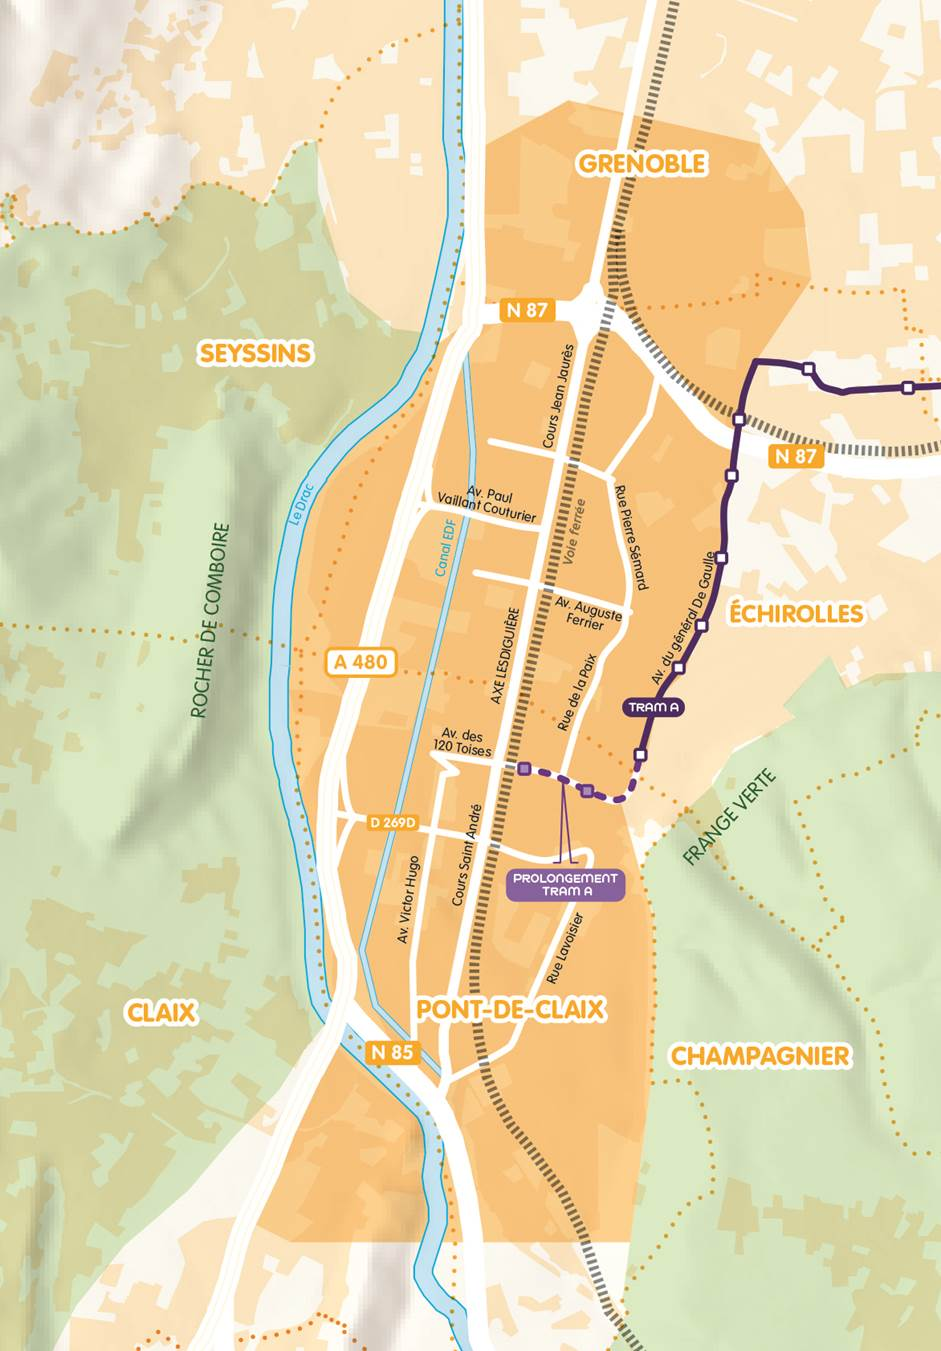
\includegraphics[width=\textwidth]{figures/1072_261_extension-ligne-A-tramway.jpeg}
	\end{column}
	\hspace{0.1cm}
	\begin{column}{0.7\textwidth}
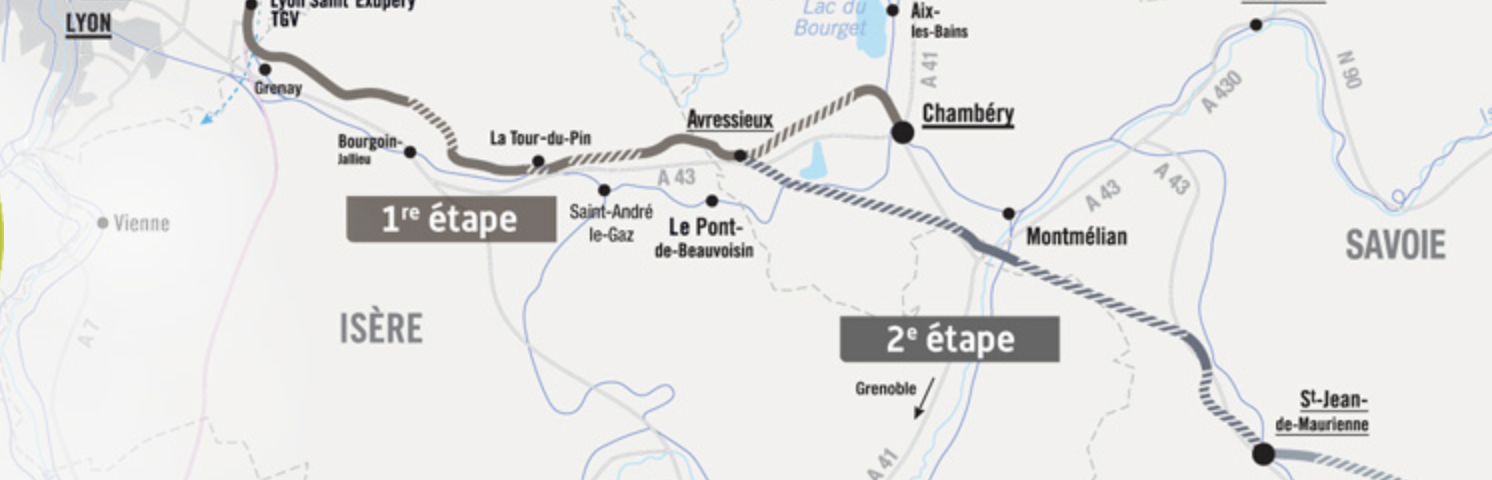
\includegraphics[width=\textwidth]{figures/lyonturin.png}
	\end{column}
	
\end{columns}

\bigskip

\footnotesize

\textit{Sources: Metropole Grenoble-Alpes \url{www.lametro.fr}; SNCF Projet Lyon-Turin \url{http://www.lyon-turin.info}}

}


\sframe{Interactions entre réseaux et territoires}{


\begin{center}

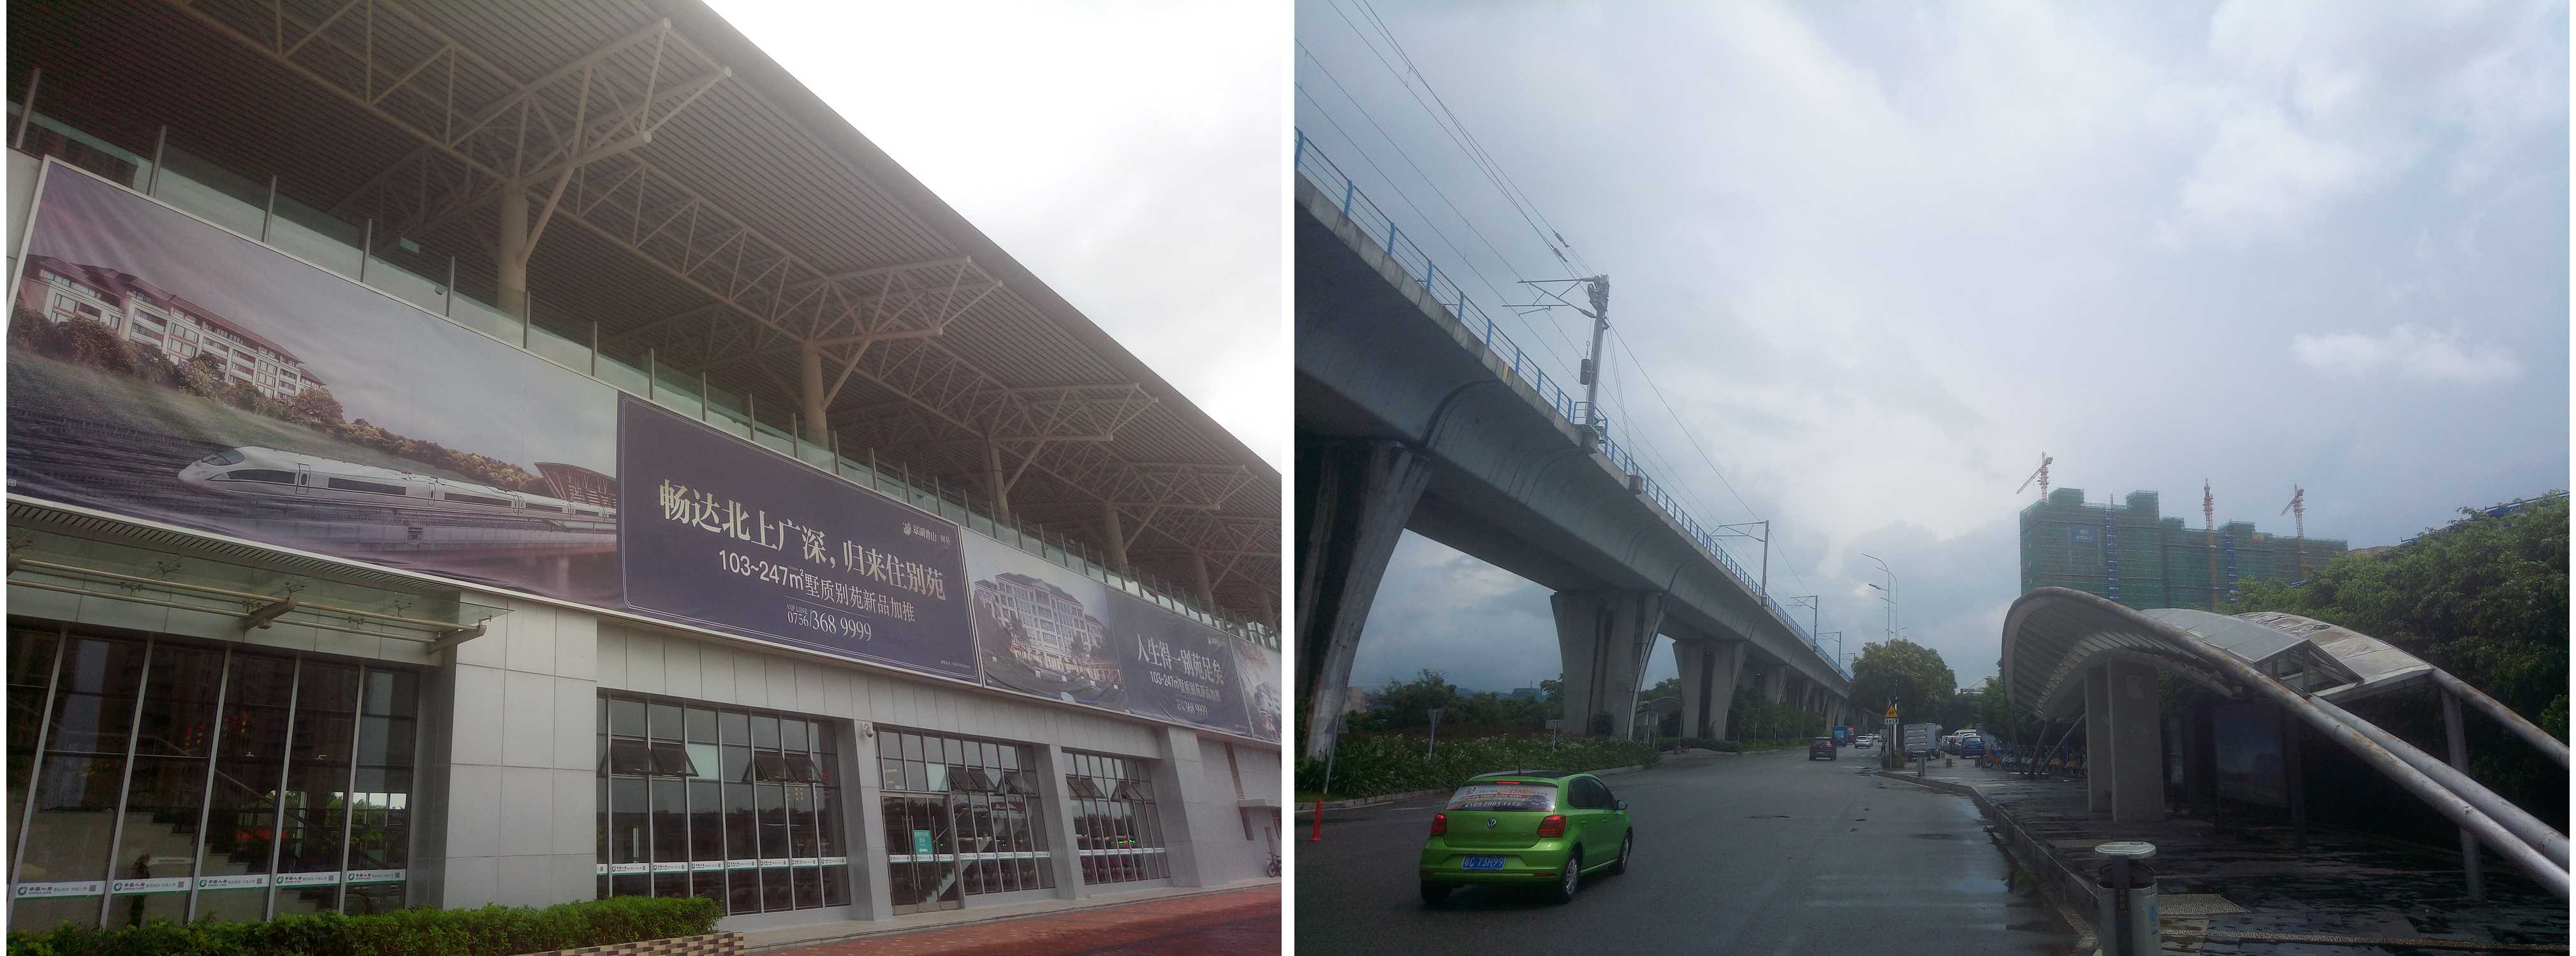
\includegraphics[width=\linewidth]{figures/example-tangjia.jpg}

\end{center}

\medskip

%\begin{justify}
\textit{Observation d'interactions entre transport et ville dans le Delta\\
de la Rivière des Perles : promotion de la grande vitesse,\\
développement urbain ciblé autour des gares.}
%\end{justify}

}



\sframe{Une approche des interactions par la co-evolution}{


Des dynamiques \textit{co-évolutives} entre réseaux de transport et territoires suggérées par de nombreux travaux (Théorie Evolutive des Villes).

\bigskip

\textbf{Axe 1 : } \textit{Comment définir et caractériser empiriquement ces dynamiques co-évolutives ?}

\bigskip

$\rightarrow$ Connaissance par les seules études empiriques qui reste limitée.
%(données pauvres, cas d'étude, temps long, couplage fort).

\bigskip

\textbf{Axe 2 : } \textit{Comment modéliser la co-évolution des réseaux de transport et des territoires ?}

\bigskip

$\rightarrow$ Utilisation de la modélisation comme outil de connaissance.


}


\sframe{Vers une modélisation ? Cartographie des disciplines}{
	
	%\vspace{-0.5cm}
	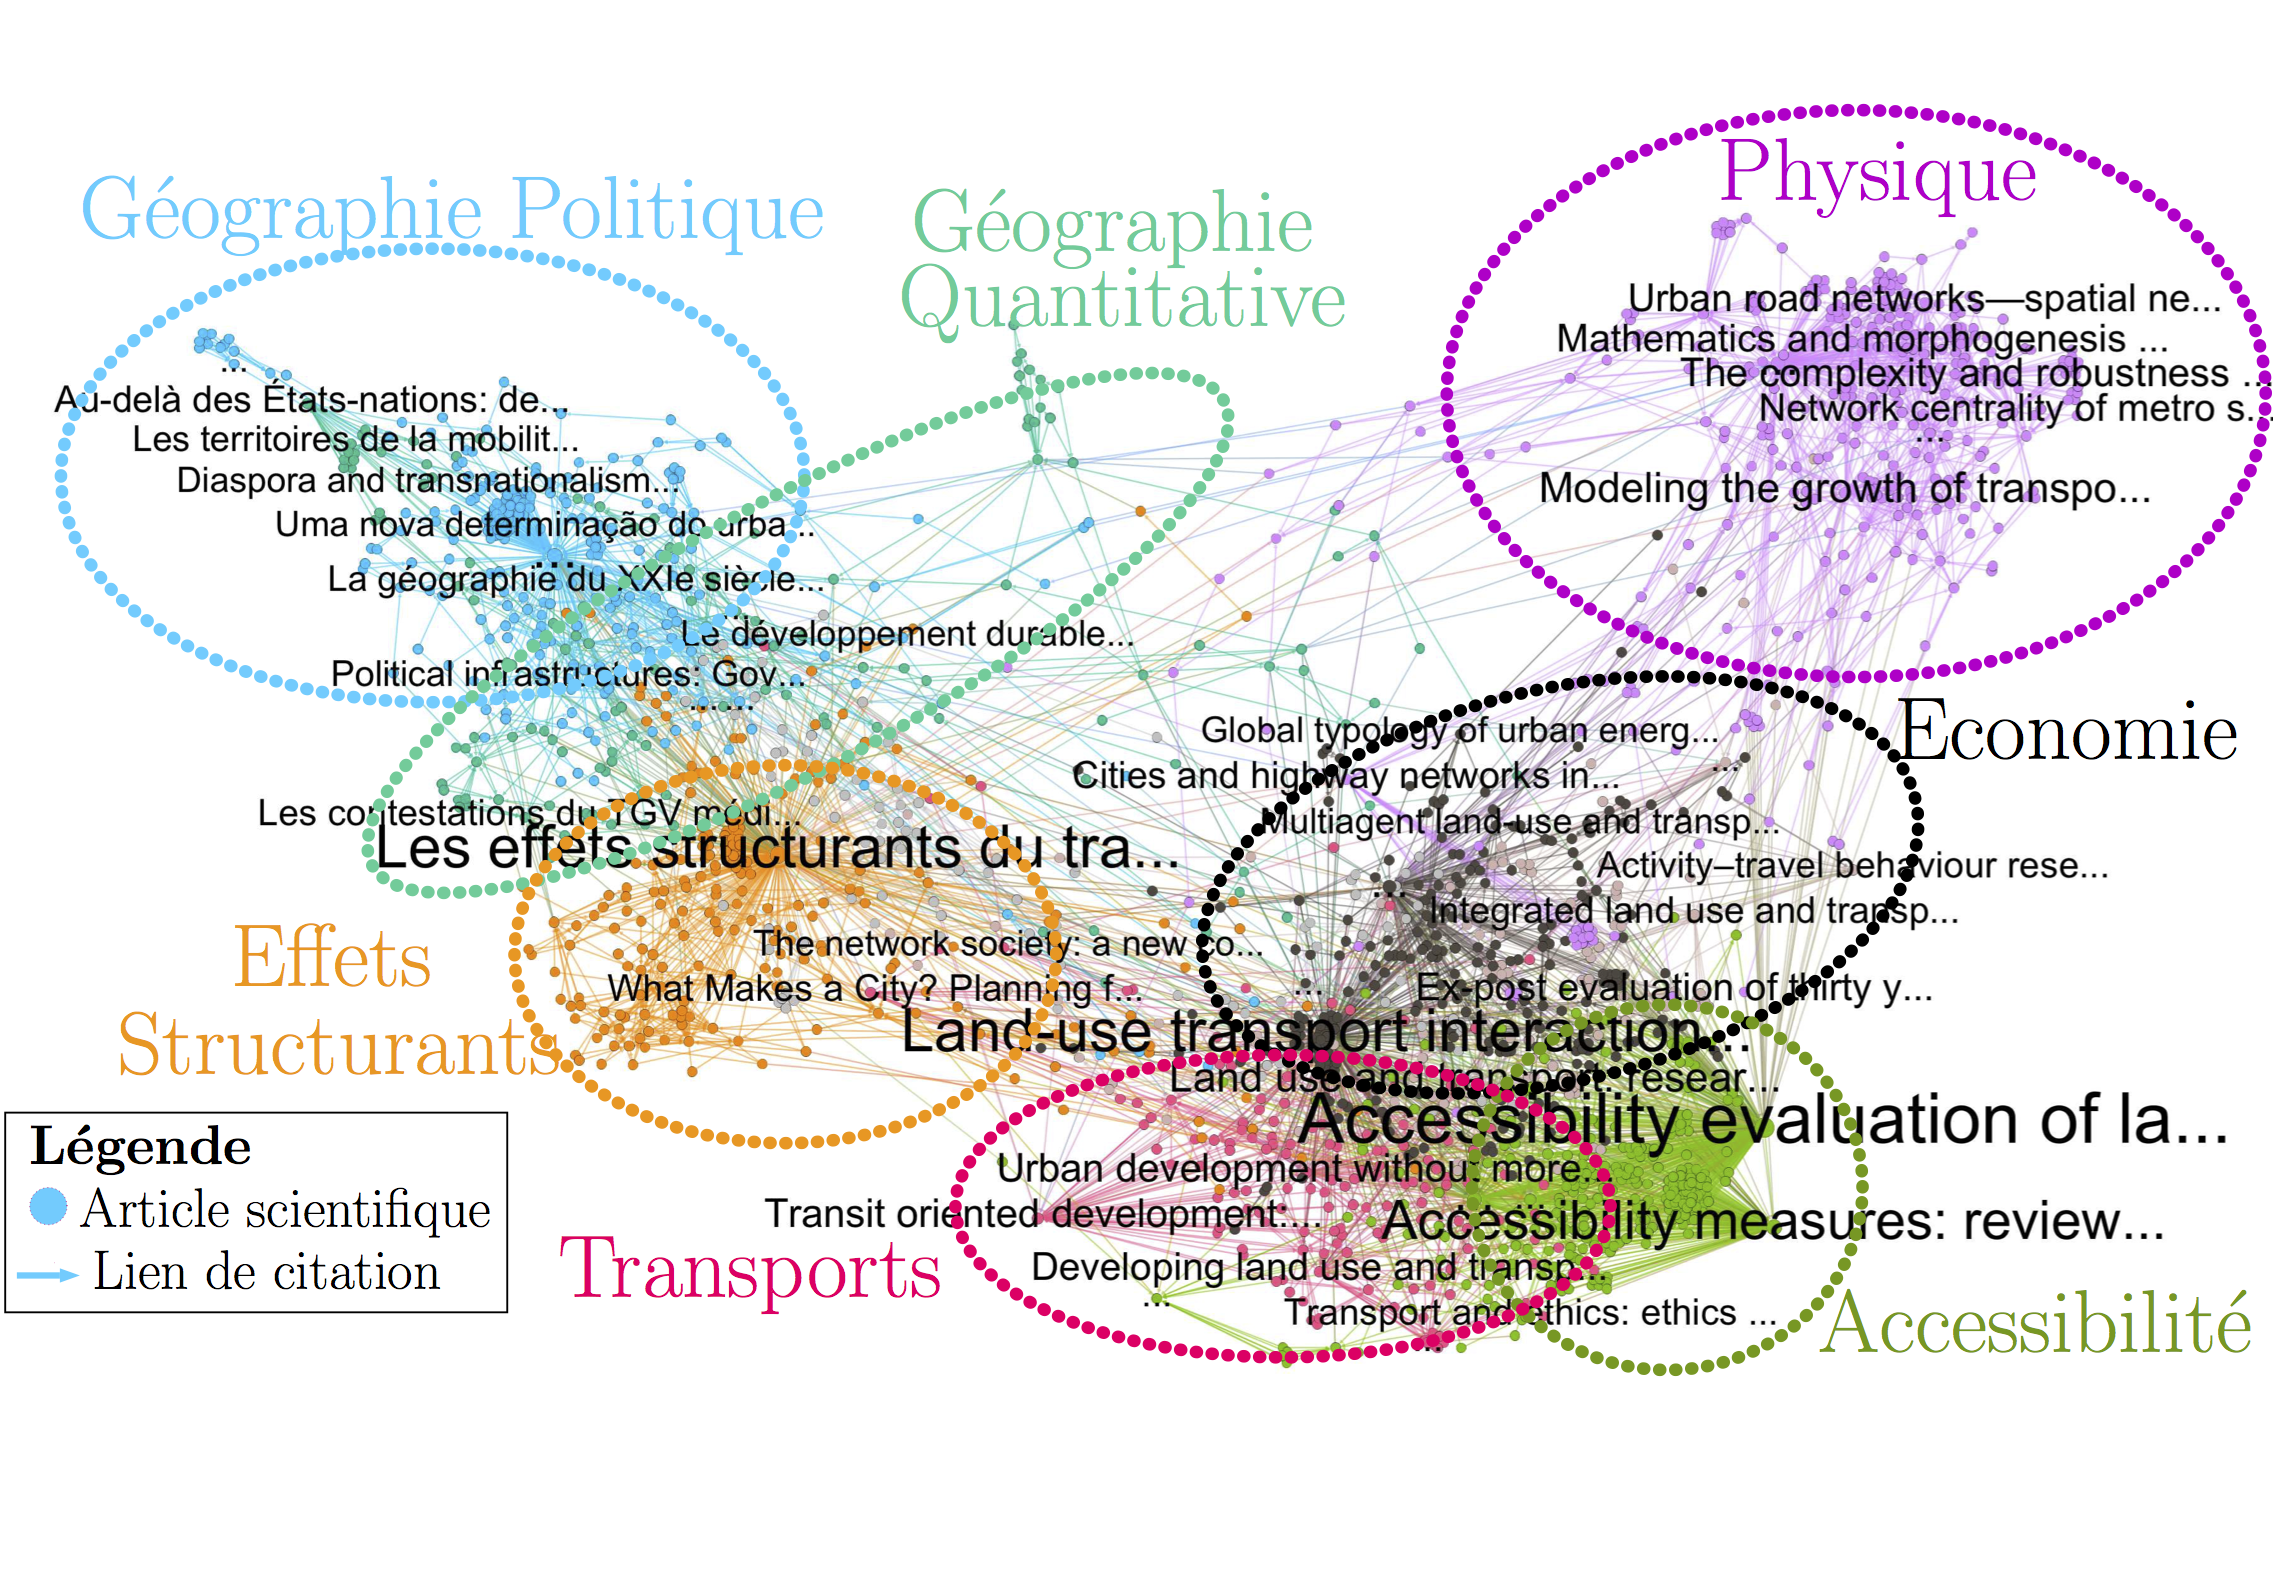
\includegraphics[width=\linewidth]{figures/quantep-graph.png}
	
	\vspace{-1cm}
	\textit{Multiples points de vue sur les mêmes objets,\\
	 autant de façons complémentaires de les modéliser.}
}



\sframe{Co-évolution: revue multidisciplinaire}{

\textit{Concept de co-évolution mobilisé par de nombreuses disciplines :}

\smallskip

\begin{itemize}
	\item Biologie : définition originale \cite{durham1991coevolution} ; concept de co-évolution diffuse \cite{strauss2005toward}
	\item Evolution culturelle \cite{Mesoudi25072017}
	\item Sociologie \cite{volberda2003co}
	\item Economie géographique \cite{schamp201020}
	\item Géographie: théorie évolutive des villes \cite{pumain1997pour}
	\item Niches écologiques \cite{holland2012signals}
\end{itemize}

\bigskip

\textbf{Concepts essentiels :}

\smallskip

(i) présence d'entités évolutives ; (ii) aux interactions plus ou moins circulaires ; (iii) dans des sous-systèmes territoriaux.

}




\sframe{Co-évolution des territoires et des réseaux: définitions}{
 
  \textbf{Objets : } 
  
  \begin{itemize}
  	\item Villes et territoires lus au prisme de la \textit{Théorie Evolutive des Villes}
  	\item Réseaux de transport comme matérialisation de ``projets transactionnels'', suivant la \textit{Théorie Territoriale des Réseaux}
  \end{itemize}
 
 \bigskip

\uncover<2->{

\textbf{Processus : }

\textit{Une définition de la co-évolution à trois niveaux : } 
\begin{enumerate}
	\item \textcolor{Blue}{niveau des agents}
	\item \textcolor{Green}{niveau des populations d'agents (niches)}
	\item \textcolor{Red}{niveau global du système}
\end{enumerate}  

}

\bigskip

\uncover<3->{

\textbf{Entrées : }

\begin{enumerate}
	\item \textcolor{Blue}{Entrée empirique (niveau microscopique)}
	\item \textcolor{Green}{Entrée par la morphogenèse (niveau de la niche)}
	\item \textcolor{Red}{Entrée par la théorie évolutive (niveau global)}
\end{enumerate}

}
 
 
}




%%%%%
%% Slide overview modeles
%%%%%

\sframe{Aperçu des contributions en modélisation}{
	
	
	\textbf{Echelle macroscopique :}
	\begin{itemize}
		%\item \only<3->{\begin{mdframed}[linecolor=red]}\noindent Modèles d'interaction entre villes incluant le réseau \only<3->{\end{mdframed}}
		\item Modèles d'interaction entre villes incluant le réseau
		
		$\rightarrow$ \textit{Démonstration d'effets de réseau ; exploration\\
		 des régimes d'interaction}
	\end{itemize}

	\bigskip
	
	\uncover<2->{
	\textbf{Echelle mesoscopique :}
	\begin{itemize}
		\item Modèle de morphogenèse couplant forme urbaine et réseau
		
		 $\rightarrow$ \textit{Complémentarité de multiples processus ; calibration au premier et second ordre}
		\item Extension et exploration du modèle Lutecia, incluant la gouvernance du système de transport
	\end{itemize}
}
	
}





%%%%%
%% Slides macro
%%%%%



\sframe{Modèle macroscopique d'interaction}{

\begin{pspicture}(0,-2.91)(11.46,2.91)
\definecolor{colour0}{rgb}{0.2,0.6,0.0}
\definecolor{colour1}{rgb}{1.0,0.0,0.2}
\definecolor{colour2}{rgb}{0.0,0.4,0.8}
\pscircle[linecolor=black, linewidth=0.04, dimen=outer](0.8,0.29){0.8}
\pscircle[linecolor=black, linewidth=0.04, dimen=outer](3.44,-1.87){0.38}
\pscircle[linecolor=black, linewidth=0.04, dimen=outer](4.64,2.11){0.5}
\pscircle[linecolor=black, linewidth=0.04, dimen=outer](6.72,-2.09){0.48}
\rput[bl](0.28,0.39){\textit{Ville 1}}
\rput[bl](4.16,2.67){\textit{Ville 2}}
\rput[bl](2.88,-2.63){\textit{Ville 3}}
\rput[bl](6.16,-2.91){\textit{Ville 4}}
\pscircle[linecolor=black, linewidth=0.04, dimen=outer](7.56,2.49){0.44}
\pscircle[linecolor=black, linewidth=0.04, dimen=outer](7.56,2.39){0.34}
\pscircle[linecolor=black, linewidth=0.04, dimen=outer](7.56,2.29){0.22}
\rput[bl](8.18,2.19){Population}
\only<2->{
\psline[linecolor=black, linewidth=0.04, linestyle=dashed, dash=0.17638889cm 0.10583334cm](1.52,-0.11)(3.56,-1.27)(6.24,-1.99)
\psline[linecolor=black, linewidth=0.04, linestyle=dashed, dash=0.17638889cm 0.10583334cm](1.5,0.65)(4.14,1.89)
\psline[linecolor=black, linewidth=0.04, linestyle=dashed, dash=0.17638889cm 0.10583334cm](4.86,1.67)(6.42,-1.67)
\psline[linecolor=black, linewidth=0.04, linestyle=dashed, dash=0.17638889cm 0.10583334cm](3.54,-1.49)(4.46,1.65)
}
\only<3->{
\rput{-26.454165}(-0.3952402,0.39846048){\psarc[linecolor=colour0, linewidth=0.04, dimen=outer, arrowsize=0.05291667cm 2.0,arrowlength=1.4,arrowinset=0.0]{<-}(0.65,1.04){0.34}{25.401218}{227.9924}}
\psarc[linecolor=colour0, linewidth=0.04, dimen=outer, arrowsize=0.05291667cm 2.0,arrowlength=1.4,arrowinset=0.0]{<-}(4.08,2.13){0.28}{63.434948}{284.03625}
\psarc[linecolor=colour0, linewidth=0.04, dimen=outer, arrowsize=0.05291667cm 2.0,arrowlength=1.4,arrowinset=0.0]{<-}(3.0,-1.91){0.24}{54.162346}{315.0}
\rput{132.8386}(10.745382,-8.510234){\psarc[linecolor=colour0, linewidth=0.04, dimen=outer, arrowsize=0.05291667cm 2.0,arrowlength=1.4,arrowinset=0.0]{<-}(7.23,-1.91){0.41}{126.483}{346.42313}}
\psline[linecolor=colour0, linewidth=0.04, arrowsize=0.05291667cm 2.0,arrowlength=1.4,arrowinset=0.0]{<-}(7.18,1.83)(8.0,1.83)
\rput[bl](8.16,1.69){Croissance endog{\`e}ne}
}
\only<4->{
\psline[linecolor=colour0, linewidth=0.08, arrowsize=0.05291667cm 2.0,arrowlength=1.4,arrowinset=0.0]{<->}(1.56,0.53)(4.18,1.77)
\psline[linecolor=colour0, linewidth=0.16, arrowsize=0.05291667cm 2.0,arrowlength=1.4,arrowinset=0.0]{<->}(1.6,0.07)(6.2,-1.85)
\psline[linecolor=colour0, linewidth=0.08, arrowsize=0.05291667cm 2.0,arrowlength=1.4,arrowinset=0.0]{<->}(4.8,1.53)(6.26,-1.73)
\psline[linecolor=colour0, linewidth=0.04, arrowsize=0.05291667cm 2.0,arrowlength=1.4,arrowinset=0.0]{<->}(1.44,-0.29)(3.16,-1.51)
\psline[linecolor=colour0, linewidth=0.04, arrowsize=0.05291667cm 2.0,arrowlength=1.4,arrowinset=0.0]{<->}(3.86,-1.91)(6.2,-2.19)
\psline[linecolor=colour0, linewidth=0.04, arrowsize=0.05291667cm 2.0,arrowlength=1.4,arrowinset=0.0]{<->}(7.18,1.37)(8.08,1.37)
\rput[bl](8.2,1.29){Interaction directe}
}
\only<5->{
\psline[linecolor=colour1, linewidth=0.04, arrowsize=0.05291667cm 2.0,arrowlength=1.4,arrowinset=0.0]{<-}(3.38,-1.47)(3.56,-0.83)
\psline[linecolor=colour1, linewidth=0.04, arrowsize=0.05291667cm 2.0,arrowlength=1.4,arrowinset=0.0]{<-}(7.239434,0.8681779)(7.940566,0.8718221)
\rput[bl](8.16,0.79){R{\'e}troaction des flux}
}
\only<6->{
\psarc[linecolor=colour2, linewidth=0.08, dimen=outer, arrowsize=0.05291667cm 2.0,arrowlength=1.4,arrowinset=0.0]{<-}(2.53,1.08){0.49}{31.297699}{206.56505}
\rput{24.443954}(0.36267212,-1.6543155){\psarc[linecolor=colour2, linewidth=0.08, dimen=outer, arrowsize=0.05291667cm 2.0,arrowlength=1.4,arrowinset=0.0]{<-}(4.0,0.01){0.3}{43.264294}{270.0}}
\rput{-24.545204}(0.48092335,2.1707923){\psarc[linecolor=colour2, linewidth=0.08, dimen=outer, arrowsize=0.05291667cm 2.0,arrowlength=1.4,arrowinset=0.0]{<-}(5.23,-0.02){0.73}{113.76878}{353.57126}}
\rput{-120.28376}(7.6030025,2.224528){\psarc[linecolor=colour2, linewidth=0.08, dimen=outer, arrowsize=0.05291667cm 2.0,arrowlength=1.4,arrowinset=0.0]{<-}(4.44,-1.07){0.46}{36.341637}{274.27374}}
\rput{-76.46916}(2.4050338,2.3124602){\psarc[linecolor=colour2, linewidth=0.08, dimen=outer, arrowsize=0.05291667cm 2.0,arrowlength=1.4,arrowinset=0.0]{->}(2.67,-0.37){0.4}{229.21208}{350.33667}}
\psline[linecolor=colour2, linewidth=0.04, arrowsize=0.05291667cm 2.0,arrowlength=1.4,arrowinset=0.0]{<-}(7.26,0.37)(7.96,0.37)
\rput[bl](8.14,0.25){Adaptation du r{\'e}seau}
}
\end{pspicture}


}



\sframe{Modèles macroscopiques : effets de réseaux}{
% - modele statique revele effets de réseaux
% - modele de co-evolution synthetique exhibe nombreux regimes, dont co-evolution, diversite plus large que modele existant dans la literature
% - deux modeles calibrés sur données fr : extrapolation effet tunnel par exemple

%Famille de modèles d'interaction dans un système de villes, basés sur les flux entre villes, incluant effets directs des flux, rétroactions par les flux traversés, rétroactions sur la vitesse du réseau.

%\vspace{1cm}

%\begin{columns}
%\begin{column}{0.35\textwidth}
	
	%\footnotesize
	
%	\textbf{Application 1 :}
%	


\centering

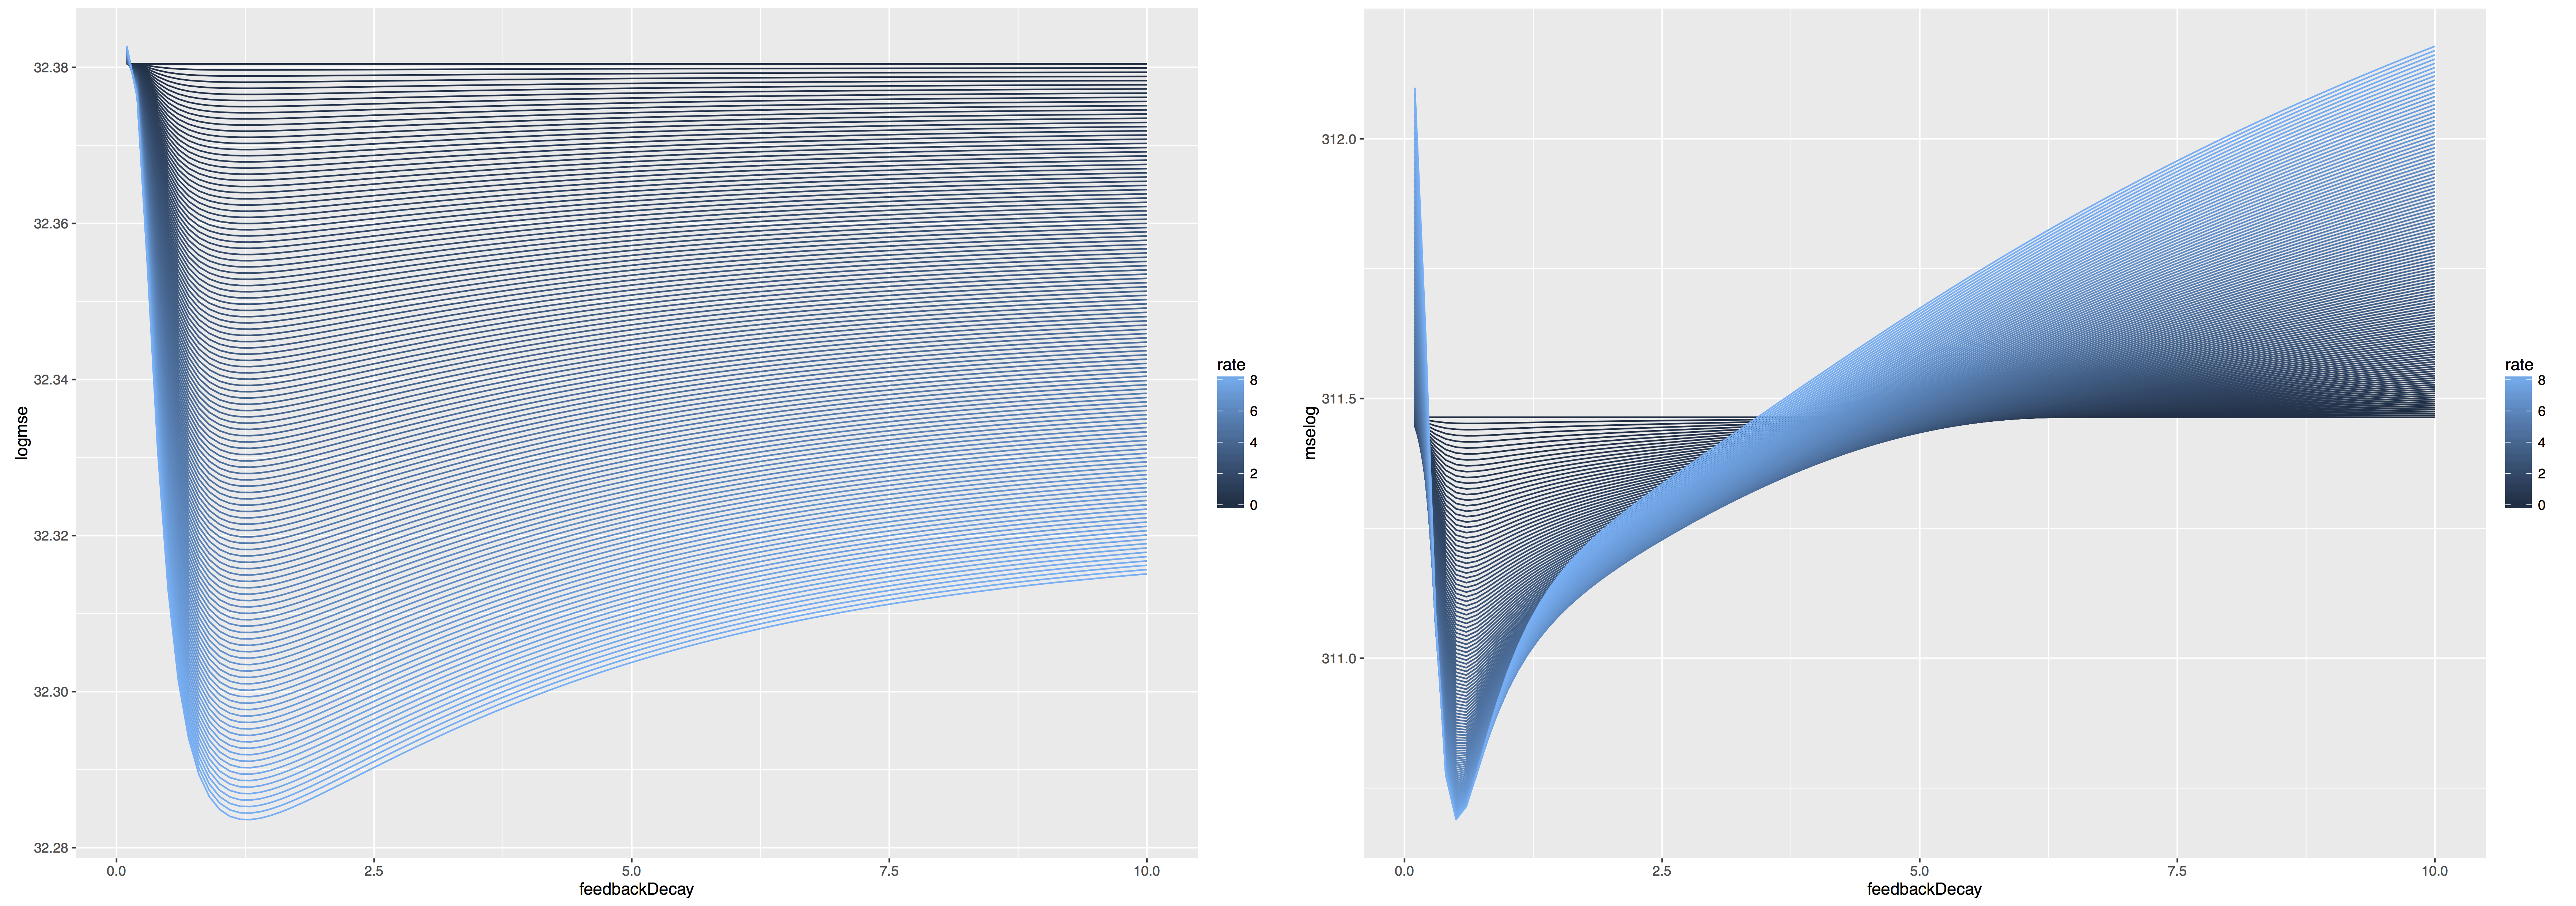
\includegraphics[width=\textwidth]{figures/intgib_Fig3.png}
	
	\bigskip
	
\raggedright
	
	\textit{Effets de réseau robustes au surapprentissage révélés par le modèle avec réseau statique} \cite{raimbault2018indirect}
	
%	\bigskip
%	\bigskip
%	
%	\centering
%
%\begin{tabular}{|l|l|l|}
%\hline
%Modèle stat.& $\Delta AIC$ & $\Delta BIC$\\
%\hline
%Polynomial &19.6&3.7\\
%Log-polynomial & 125.4& 109.4\\
%Polynomial-généralisé & 11.7& -4.2\\
%\hline
%\end{tabular}
%
%\medskip

		
%\end{column}
%\vrule
%\hspace{0.2cm}


%\vrule

%\hspace{0.2cm}

%\end{columns}
}


\sframe{Modèles macroscopiques : régimes de co-évolution}{

%\begin{column}{0.3\textwidth}

\centering

	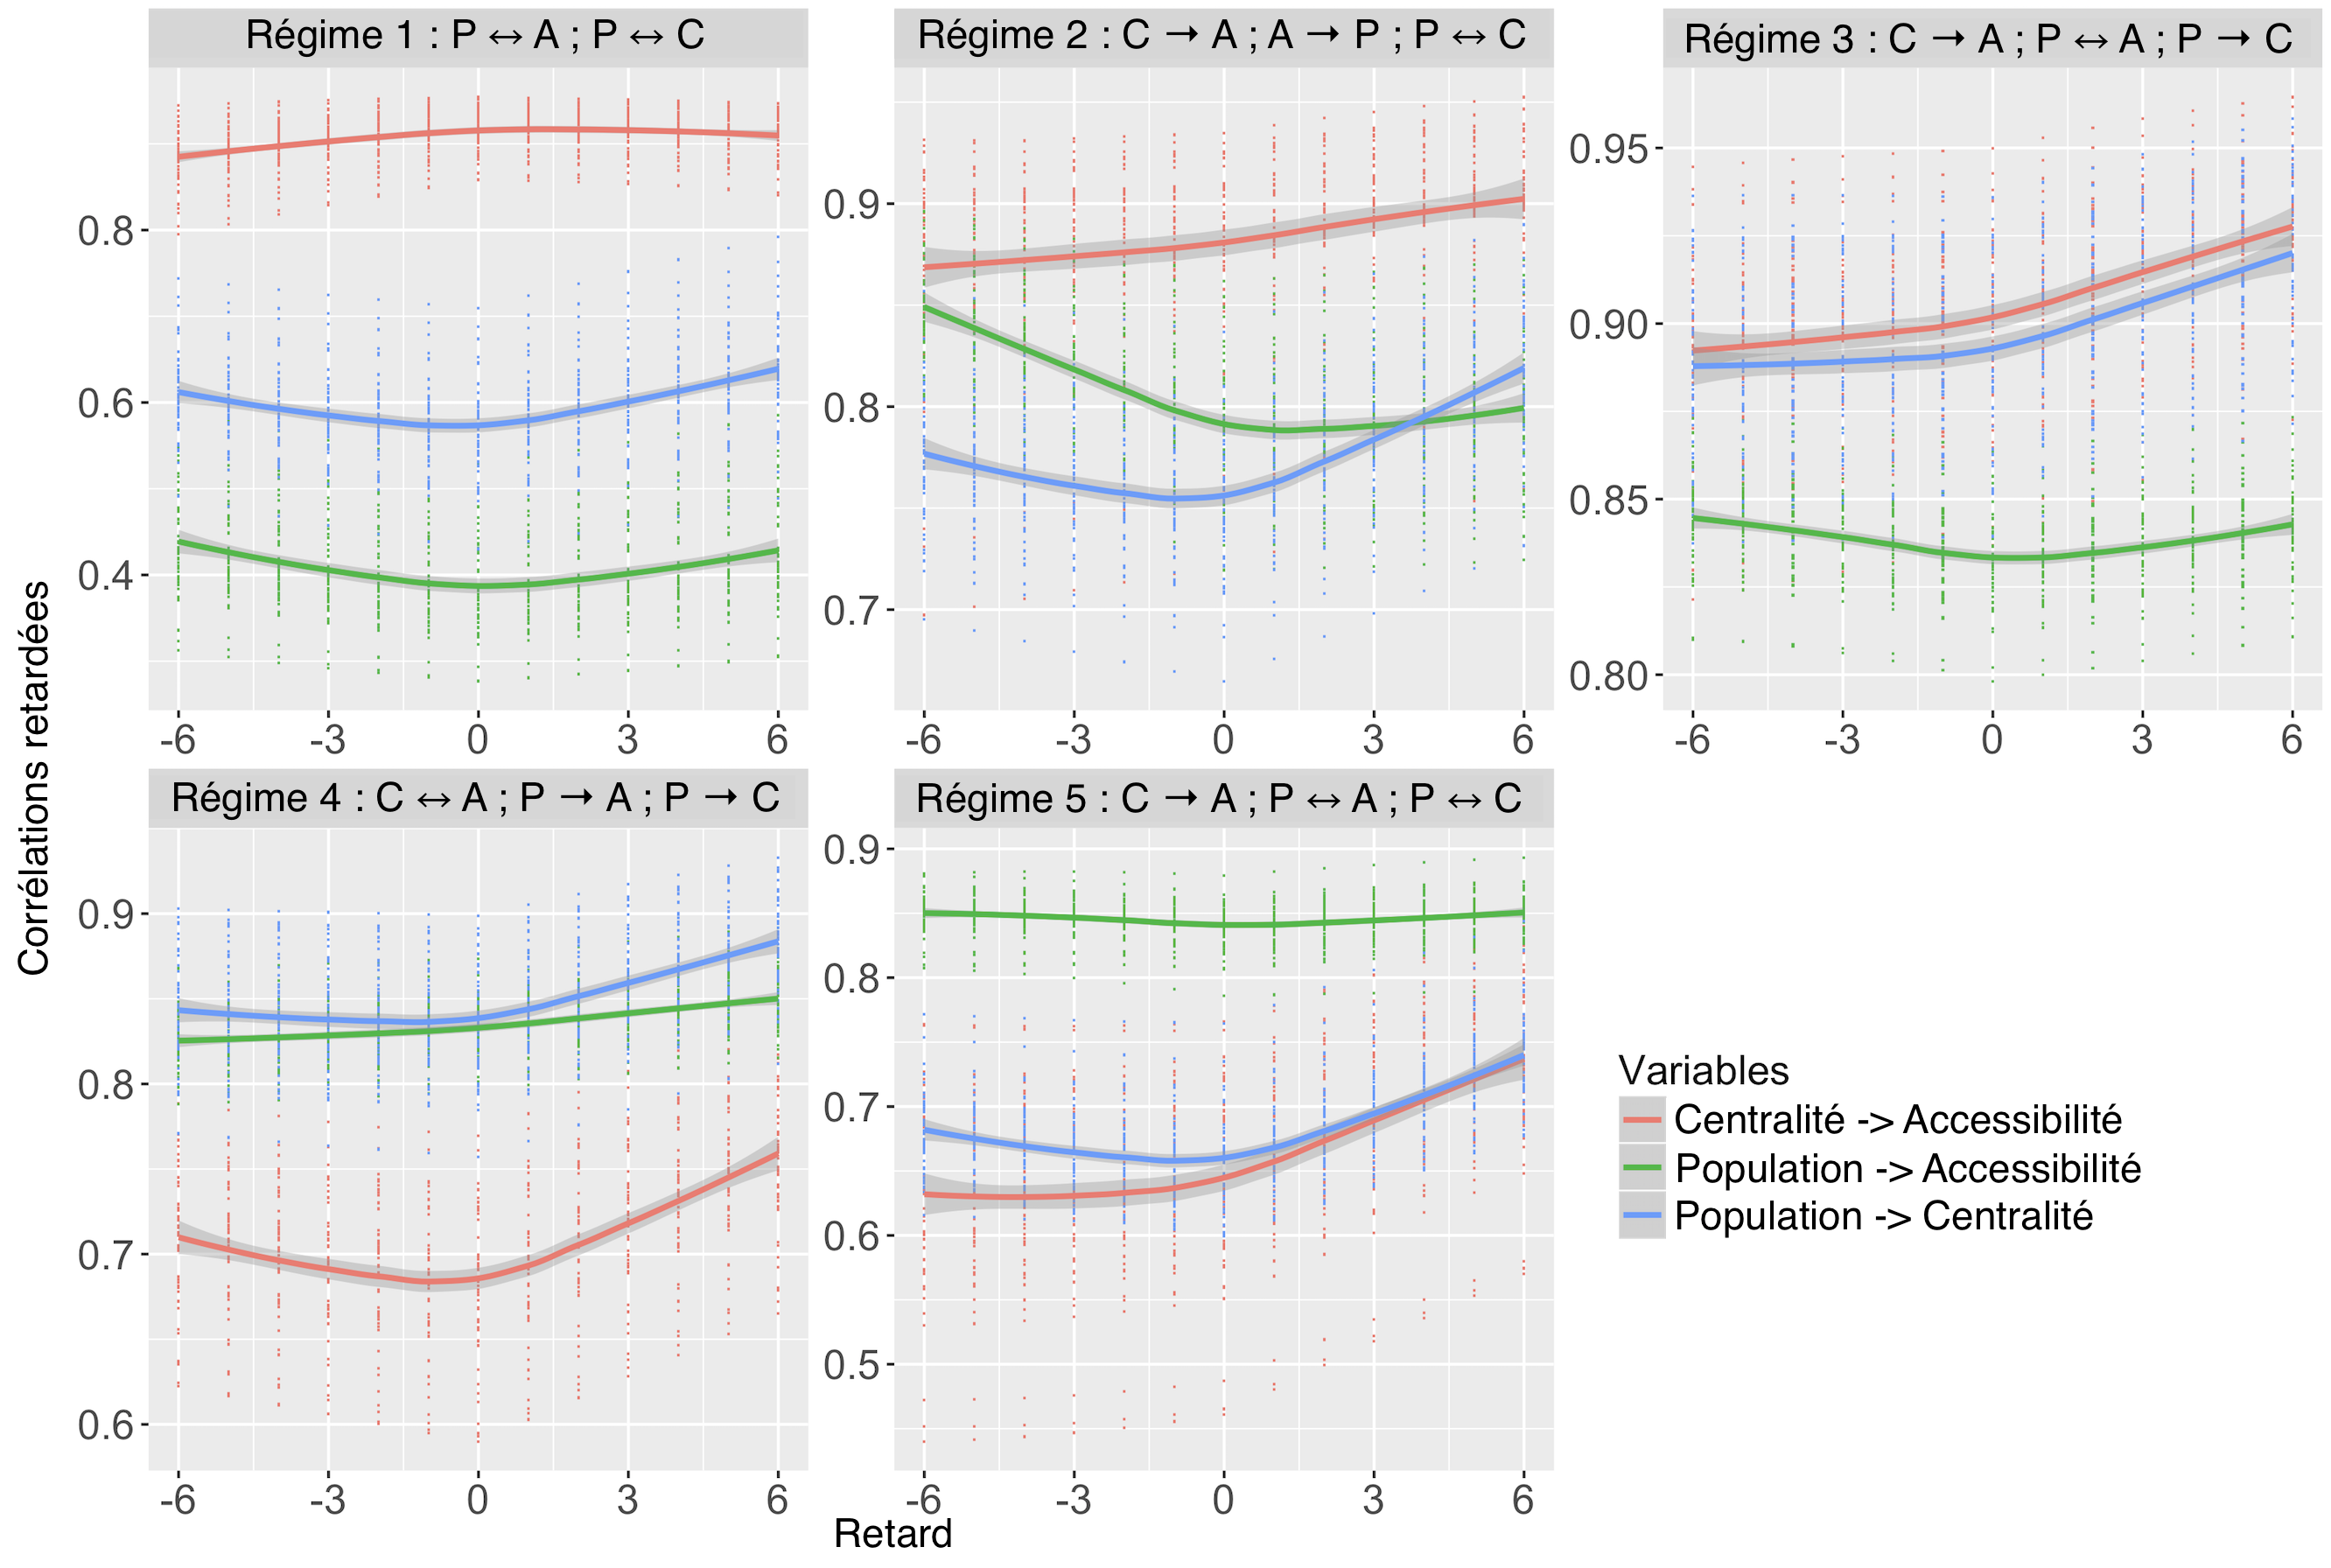
\includegraphics[width=\linewidth]{figures/macro-regimes.png}
	
	\medskip
	
	%\footnotesize
	
	%\begin{justify}

\raggedright

\vspace{-0.4cm}

	\textit{Multiples régimes mis en évidence dans des configurations synthétiques} \cite{raimbault2018modeling} 


	%\end{justify}
%\end{column}


}


%\begin{column}{0.35\textwidth}
%	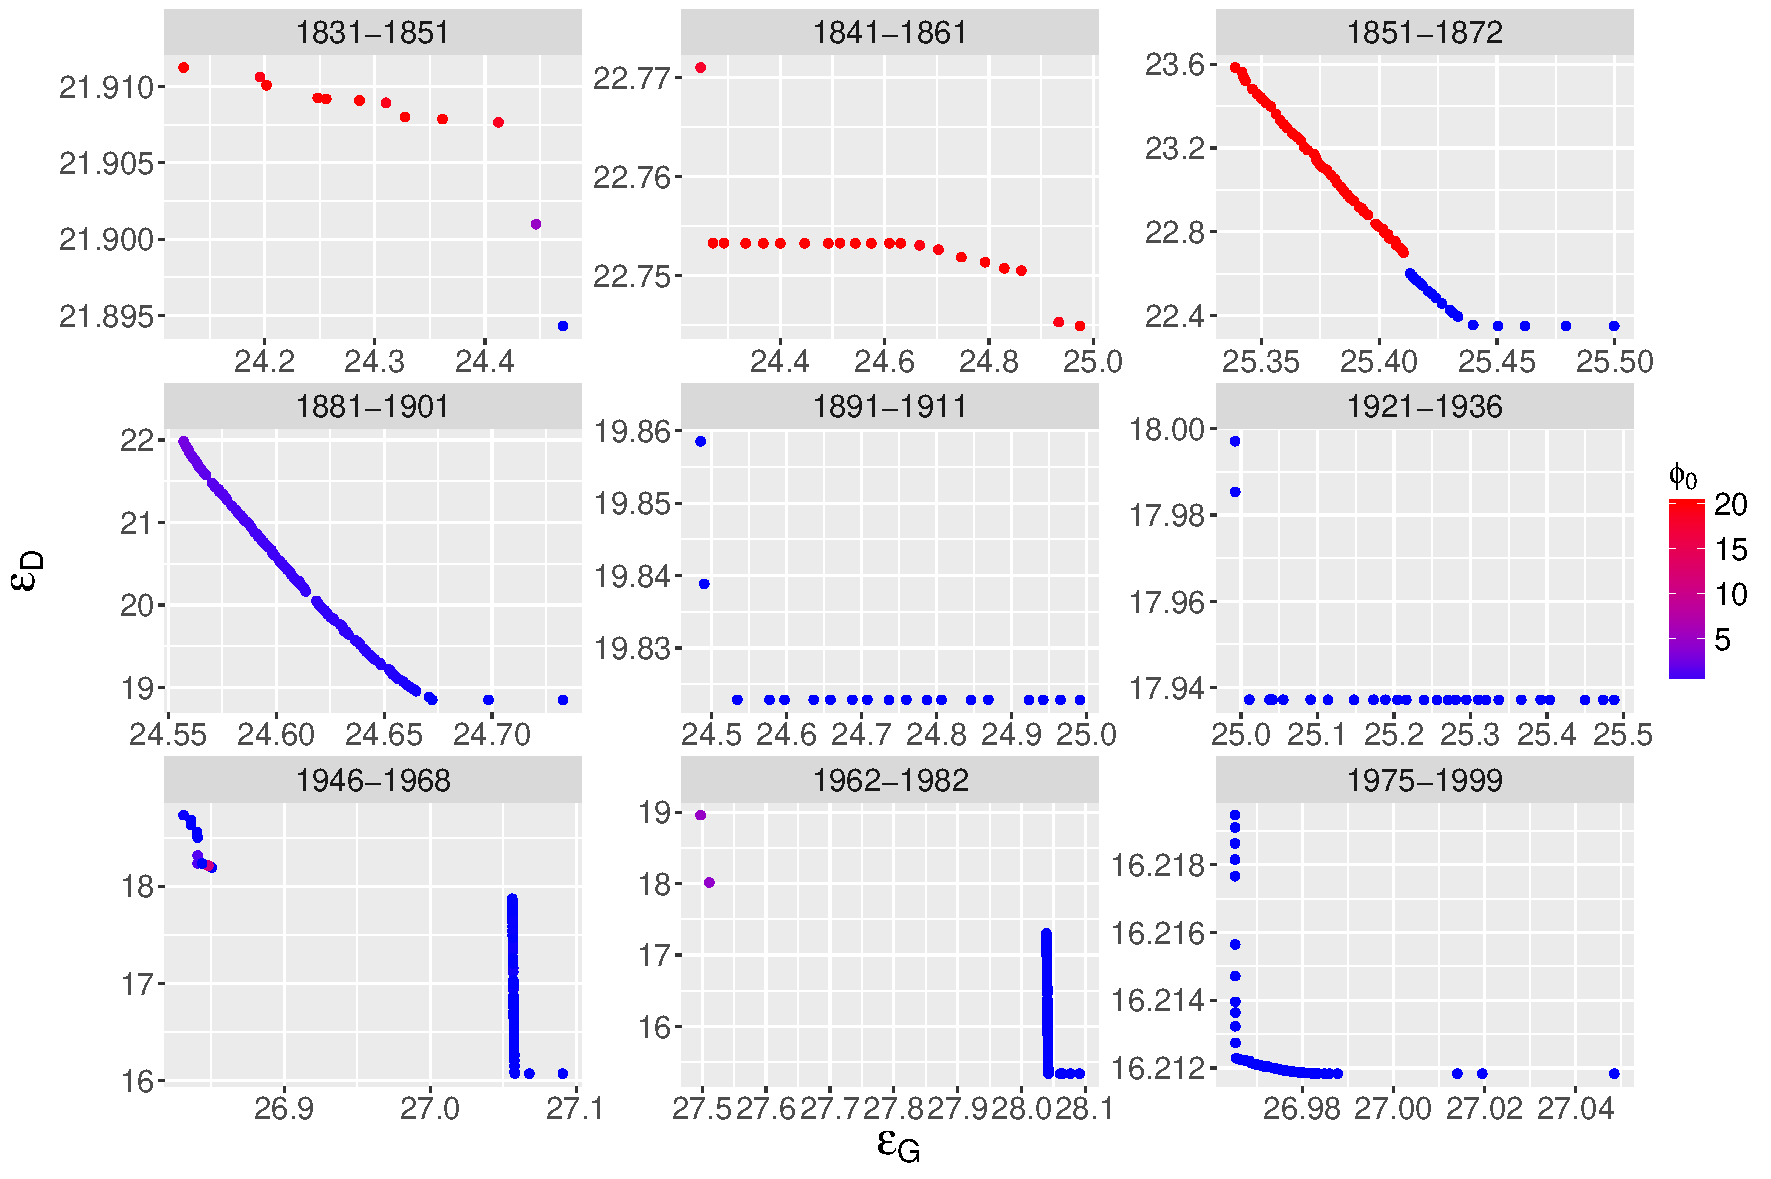
\includegraphics[width=\linewidth]{figures/9-calib.pdf}
%	
%	\medskip
%
%	\footnotesize
%
%	\begin{justify}
%	\textit{Calibration sur données de population et ferroviaires pour le système de villes français (1830-1999)}
%	\end{justify}
%\end{column}


%%%%%
%% Slide meso
%%%%%


\sframe{Modèles mesoscopiques : morphogenèse}{
%
%
%% examples : fig 2 of paper
%


\centering

\includegraphics[height=0.8\textheight]{figures/5-2-2-fig-density-fig2.jpg}

%


\footnotesize\textit{Exemples de configuration territoriales générées par un modèle d'agrégation-diffusion pour la densité de population} \cite{raimbault2018calibration}

}


\sframe{Co-évolution par morphogenèse}{


% - complementarité de multiples heuristiques de croissance de reseau
% - calibration au premier et second ordre
% - Lutecia : vers des modèles plus complexes


\footnotesize

Relation entre forme et fonction (morphogenèse) comme paradigme pour modéliser la co-évolution à l'échelle mésoscopique \cite{raimbault2018urban}

% reseau pour capturer fonction

\smallskip

%\begin{columns}
%\begin{column}{0.55\textwidth}

%\footnotesize

\justify
\textit{Un modèle par réaction-diffusion et multi-modélisation de la croissance du réseau : complémentarité des heuristiques, calibration sur les formes et leurs corrélations} 

\medskip

{\centering
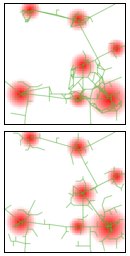
\includegraphics[width=0.3\linewidth,height=0.7\textheight]{figures/meso-nwgrowth.png}
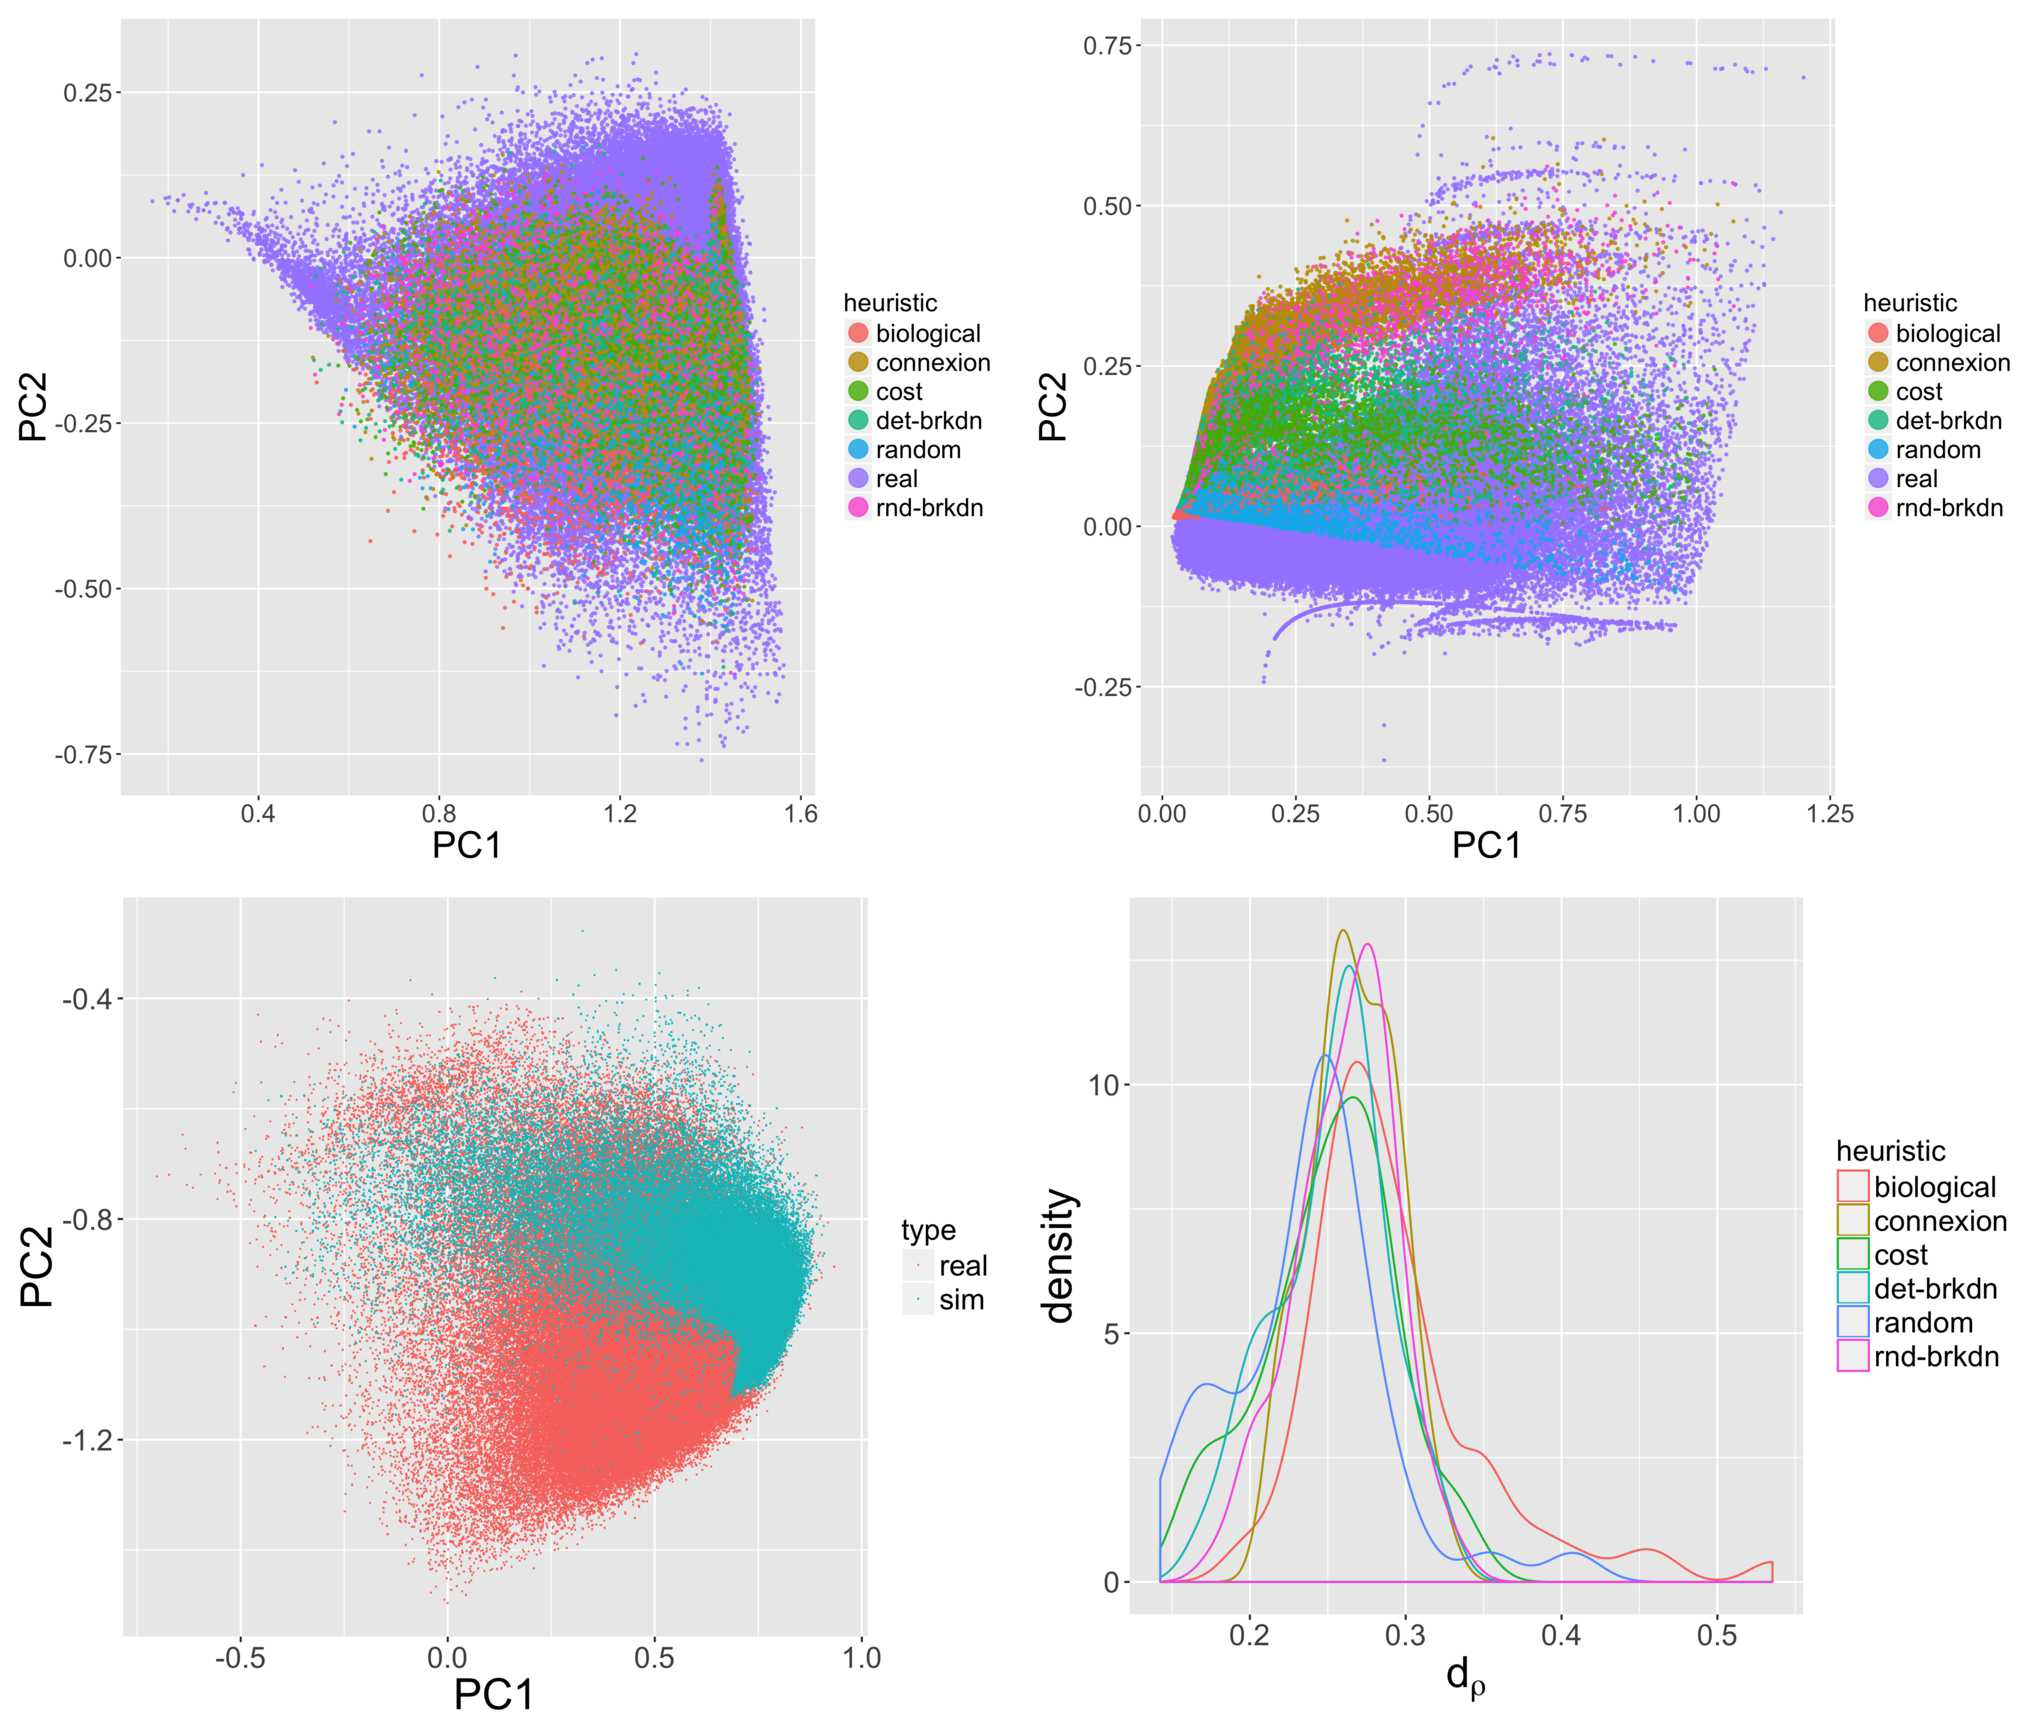
\includegraphics[width=0.7\linewidth,height=0.7\textheight]{figures/meso-calib.jpg}
}

%\medskip

%$\rightarrow$ \textit{Complémentarité des heuristiques de réseau}
%  pour reproduire des formes existantes

%$\rightarrow$ \textit{Calibration sur les formes et leurs corrélations}

%\end{column}
%\vrule
%\hspace{0.2cm}
%\begin{column}{0.35\textwidth}

%\footnotesize


}

%
\sframe{Modèles mesoscopiques}{


\textit{Le modèle Lutecia : vers une prise en compte de la gouvernance pour la croissance des réseaux de transport} \cite{lenechet:halshs-01272236}

\bigskip

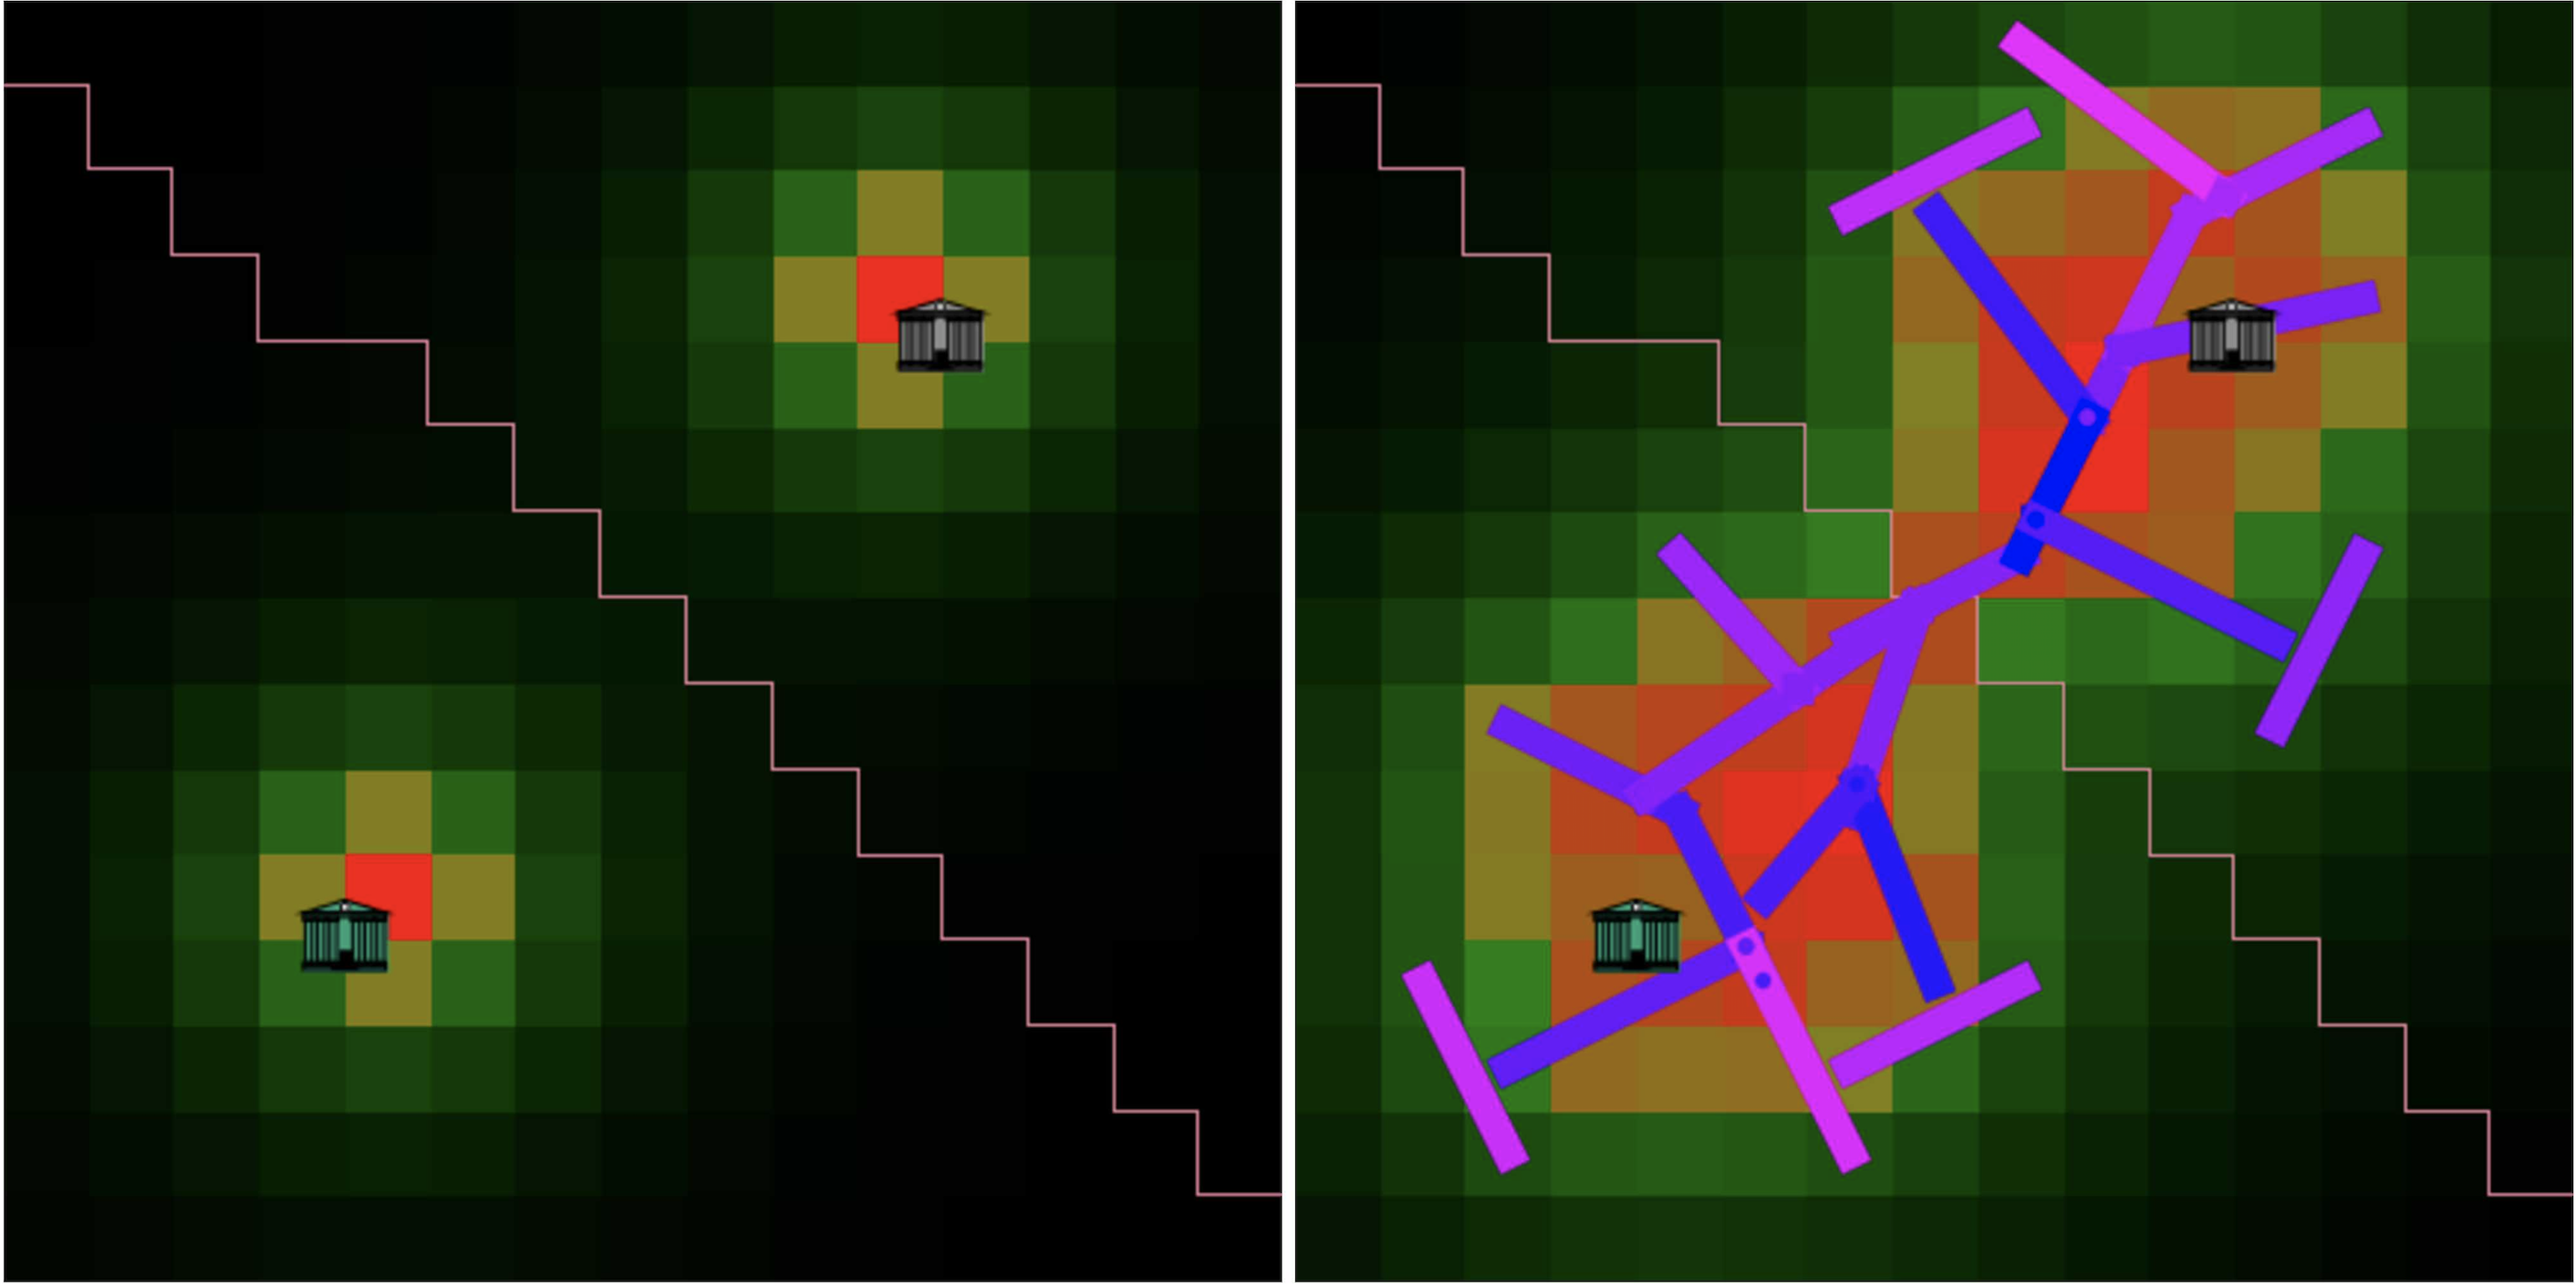
\includegraphics[width=\linewidth]{figures/meso-lutecia.jpg}




%\end{column}
%\end{columns}

}


\sframe{Calibration des modèles}{

%Bi-objective calibration of 7 models for 7 city systems $\rightarrow$ use of genetic algorithms on grid, made smooth with the OpenMOLE software \url{https://next.openmole.org/}

Utilisation de calcul intensif sur grille pour l'exploration et la calibration des modèles, rendue transparente par l'utilisation du logiciel OpenMOLE \url{https://next.openmole.org/}


\centering

\smallskip


\includegraphics[height=0.35\textheight]{figures/openmole.png}

\smallskip

\raggedright\justify

%\footnotesize
\textit{OpenMOLE: (i) embarque n'importe quel modèle ; (ii) permet un accès transparent aux environnements de calcul intensif ; (iii) fournit des méthodes pour l'exploration et la calibration des modèles de simulation.}

\bigskip

\textbf{Candidatures encore ouvertes pour l'école d'été !} 
\\(\texttt{https://exmodelo.org/})

}




\section{Perspectives}

\sframe{Perspectives}{

% Vers des théories intégratives des systèmes territoriaux

% donner des pistes
% theorique, epistemo quanti
% ici parler des developpements Lutecia : modeles.
% multi-modeling
%. -> bien parler de tous les domaines.
%. certains elements plus tangibles : va dans le sens de Morency : compris que quelque chose ici. : strqtgeie explorqtion ; redeveloppement langages scalable. : fait comprendre que chapitre creuser pas possible tel quel, passage a l'echelle necessaire, etc.
% 
% slide de fin : riche, permet ouverture.
%
% 

%\textbf{Contributions}
%\begin{itemize}
%	\item \textit{Définition :} relecture possible de la théorie évolutive, ouvre \\
%	 des ponts vers l'économie géographique
%	\item \textit{Caractérisation : } nombreuses perspectives d'applications\\
%	 en géographie, en sciences territoriales
%	\item \textit{Modélisation : } des modèles interdisciplinaires ayant vocation\\
%	à être couplés et réutilisés
%\end{itemize}
%\bigskip


\textbf{Echelle macroscopique}

	\begin{itemize}
		\item Approche multiplexe pour les modes de transport
		\item Vers des modèles génériques d'interaction pour les systèmes de villes \cite{raimbault2018systematic} 
	\end{itemize}

\medskip

\textbf{Echelle mesoscopique}

\begin{itemize}
	\item Généricité des types de formes urbaines
 	\item Vers des modèles opérationnels à l'échelle métropolitaine (application de Lutecia)
\end{itemize}


% \item \textit{Vers des théories intégrées des systèmes territoriaux : } modèles multi-échelles et couplage de la théorie évolutive avec la théorie du \textit{Scaling}.

\medskip

\textbf{Vers des modèles multi-échelles}

\begin{itemize}
	\item Structure plus fine du réseau dans les modèles macroscopiques
	\item Couplage de modèles mesoscopiques au sein d'un modèle d'interaction pour la détermination des paramètres exogènes
\end{itemize}


}

%  Multi-modélisation de la co-évolution à l'échelle macroscopique
	%\item \textit{Extension des méthodes d'exploration des modèles de simulation spatiaux : } données spatiales synthétiques, multi-modélisation et surajustement, robustesse des algorithmes génériques à la stochasticité.



\section{Conclusion}


\sframe{Conclusion}{

\justify

%$\rightarrow$ Différents processus d'interaction impliqués \textbf{Comparaison des modèles.}

%\medskip

$\rightarrow$ Vers des théories intégratives des systèmes territoriaux ? \textbf{Multi-échelle.}

\medskip

$\rightarrow$ Multiples dimensions et caractéristiques urbaines ? \textbf{Interdisciplinarité.}

\bigskip

\footnotesize

\textbf{Références}

Raimbault, J. (2018). Indirect evidence of network effects in a system of cities. Environment and Planning B: Urban Analytics and City Science, 2399808318774335.

%\url{https://halshs.archives-ouvertes.fr/halshs-01788559}

\smallskip	

Raimbault, J. (2018). Calibration of a density-based model of urban morphogenesis. PloS one, 13(9):e0203516

\smallskip	

Raimbault, J. (2018). Modeling the co-evolution of cities and networks. \textit{Forthcoming in Handbook of cities and networks, Rozenblat C., Niel Z., eds.} arXiv:1804.09430.

\smallskip

Raimbault, J. (2018). An urban morphogenesis model capturing interactions between networks and territories. \textit{Forthcoming in Mathematics of Urban Morphogenesis, D'acci L., ed., Springer Birkhauser Mathematics.} arXiv :1805.05195

\smallskip

Raimbault, J. (2018). Caract{\'e}risation et mod{\'e}lisation de la co-{\'e}volution des r{\'e}seaux de transport et des territoires (Doctoral dissertation, Université Paris 7 Denis Diderot). %\url{https://halshs.archives-ouvertes.fr/tel-01857741}

\bigskip


\footnotesize{ - Code, données et résultats disponibles à\\ \texttt{https://github.com/JusteRaimbault/CityNetwork}\\
- Remerciements à \textit{European Grid Infrastructure} et ses \textit{National Grid Initiatives} (\textit{France-Grilles} en particulier) pour le support technique et l'infrastructure.

}

}





\sframe{Reserve slides}{

\centering
%
\Large
%
\textbf{Reserve Slides}
%


}



%% slide c

\sframe{Problématique et plan dans les domaines de connaissance}{

\centering
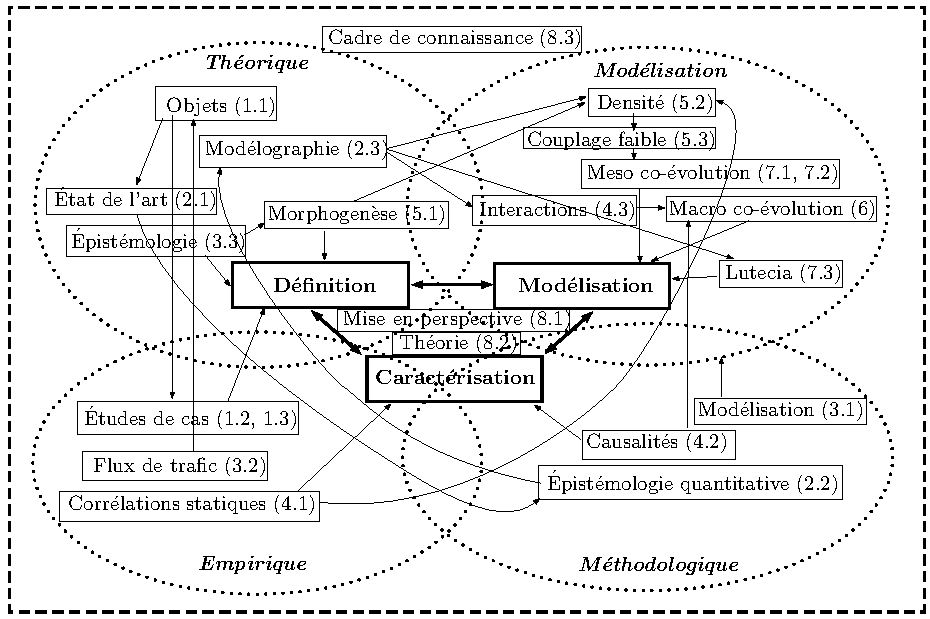
\includegraphics[width=\linewidth]{figures/domconn-organisation.pdf}

}

\sframe{Mise en perspective}{
\centering

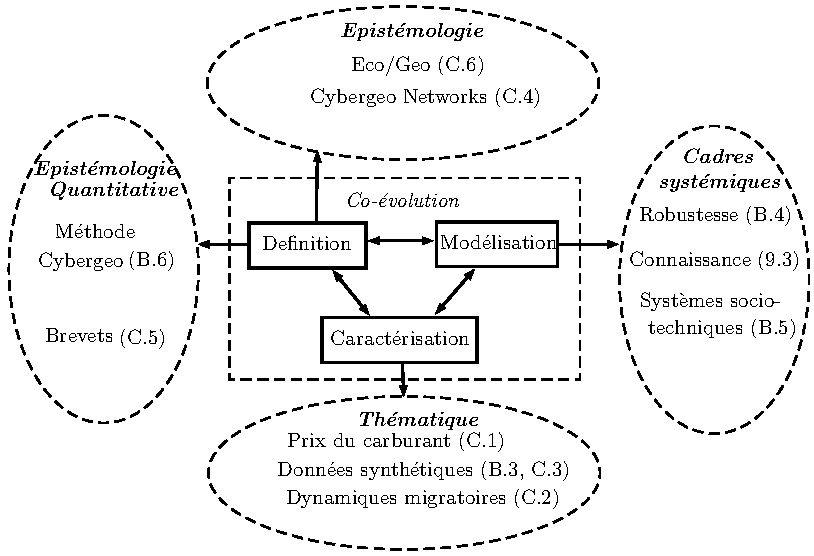
\includegraphics[width=\linewidth]{figures/opening-meta.pdf}

}



\sframe{Elaboration d'une méthode de caractérisation}{

\centering

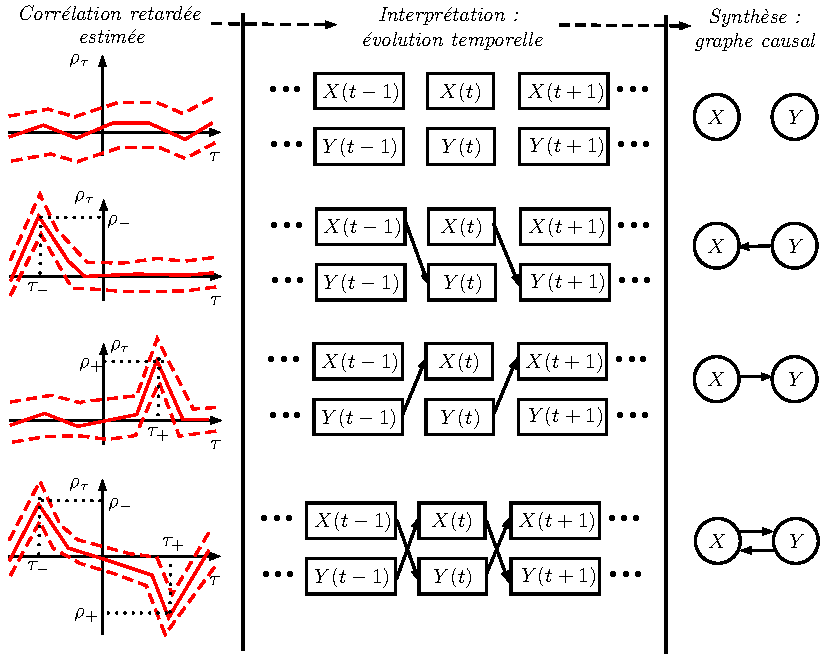
\includegraphics[width=0.9\linewidth]{figures/causality-method.pdf}

}


\sframe{Des observations empiriques contrastées}{

%Application de la méthode de caractérisation à des cas d'études à différentes échelles
%\bigskip

%\begin{columns}
%\begin{column}{0.5\textwidth}


	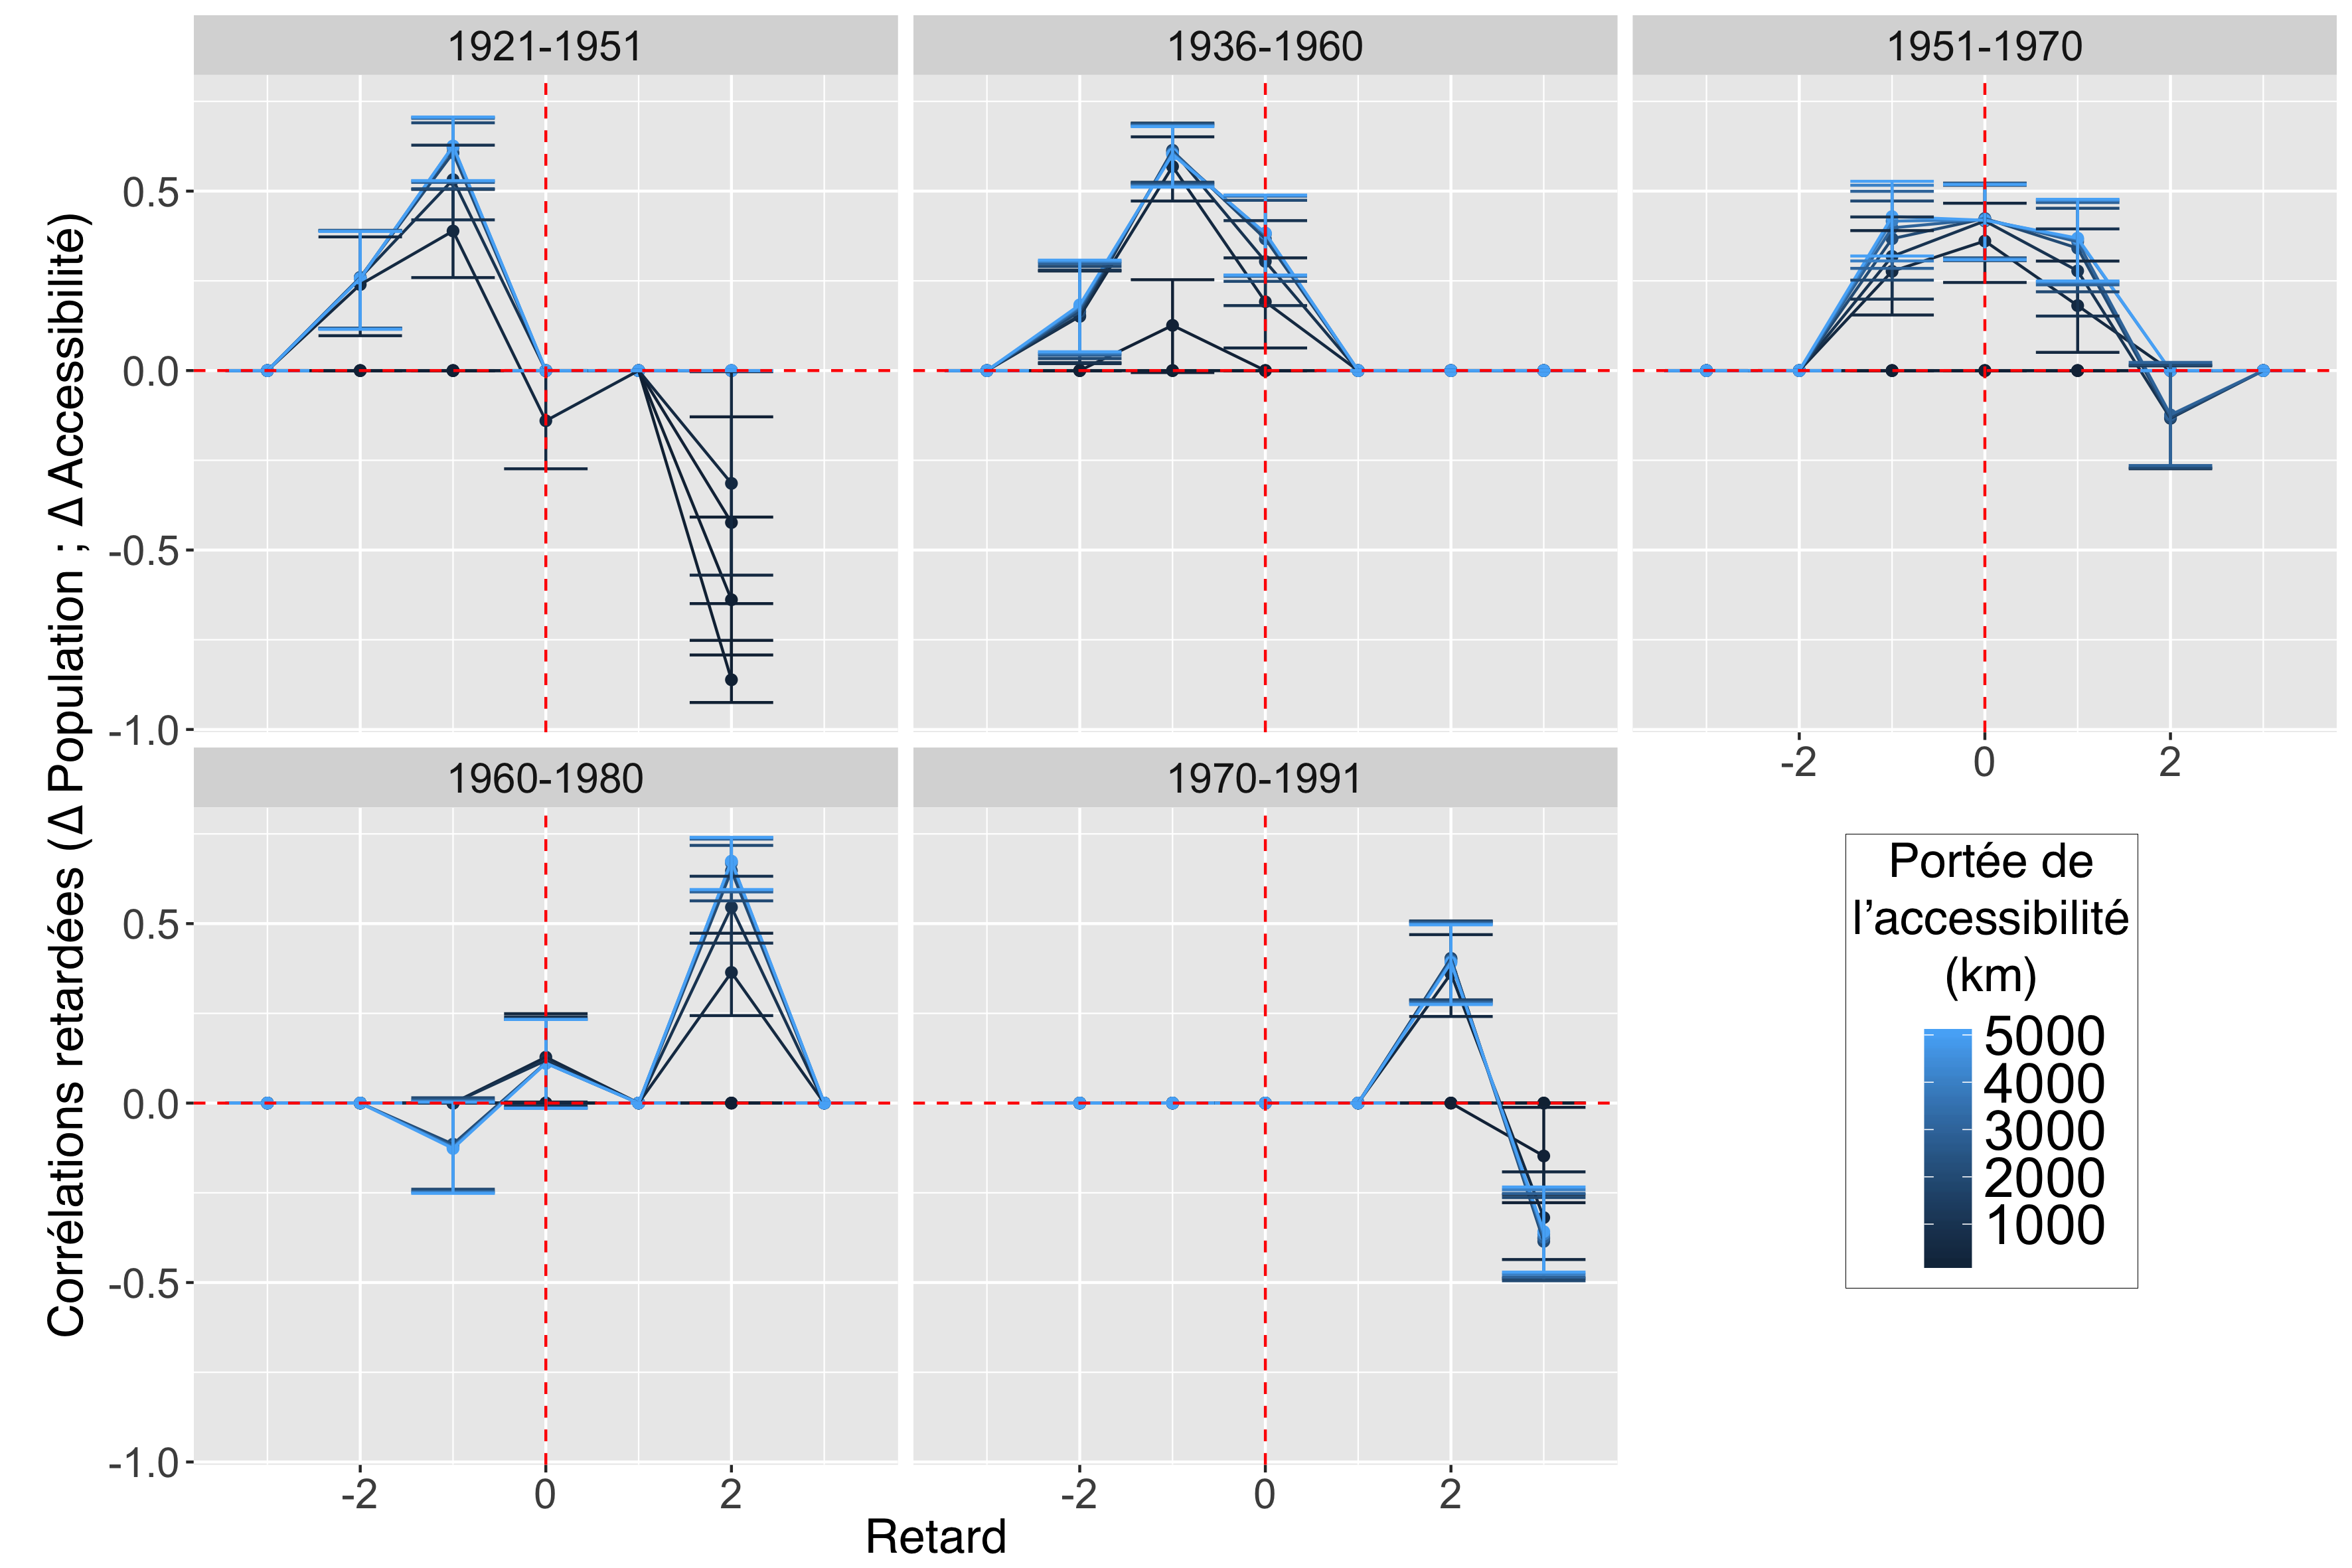
\includegraphics[width=\textwidth,height=0.8\textheight]{figures/empirical-southafrica.png}
	
	\smallskip
	
	
	\footnotesize
	
	%\vspace{-0.5cm}
	
	
	\begin{justify}
	\textit{Inversion du sens de la causalité entre croissance des populations et de l'accessibilité ferroviaire en Afrique du Sud au cours du 20ème siècle}
	\end{justify}


%\end{column}
%\vrule\hspace{0.2cm}
%	\begin{column}{0.45\textwidth}

}




\sframe{Des observations empiriques contrastées}{


\begin{center}
	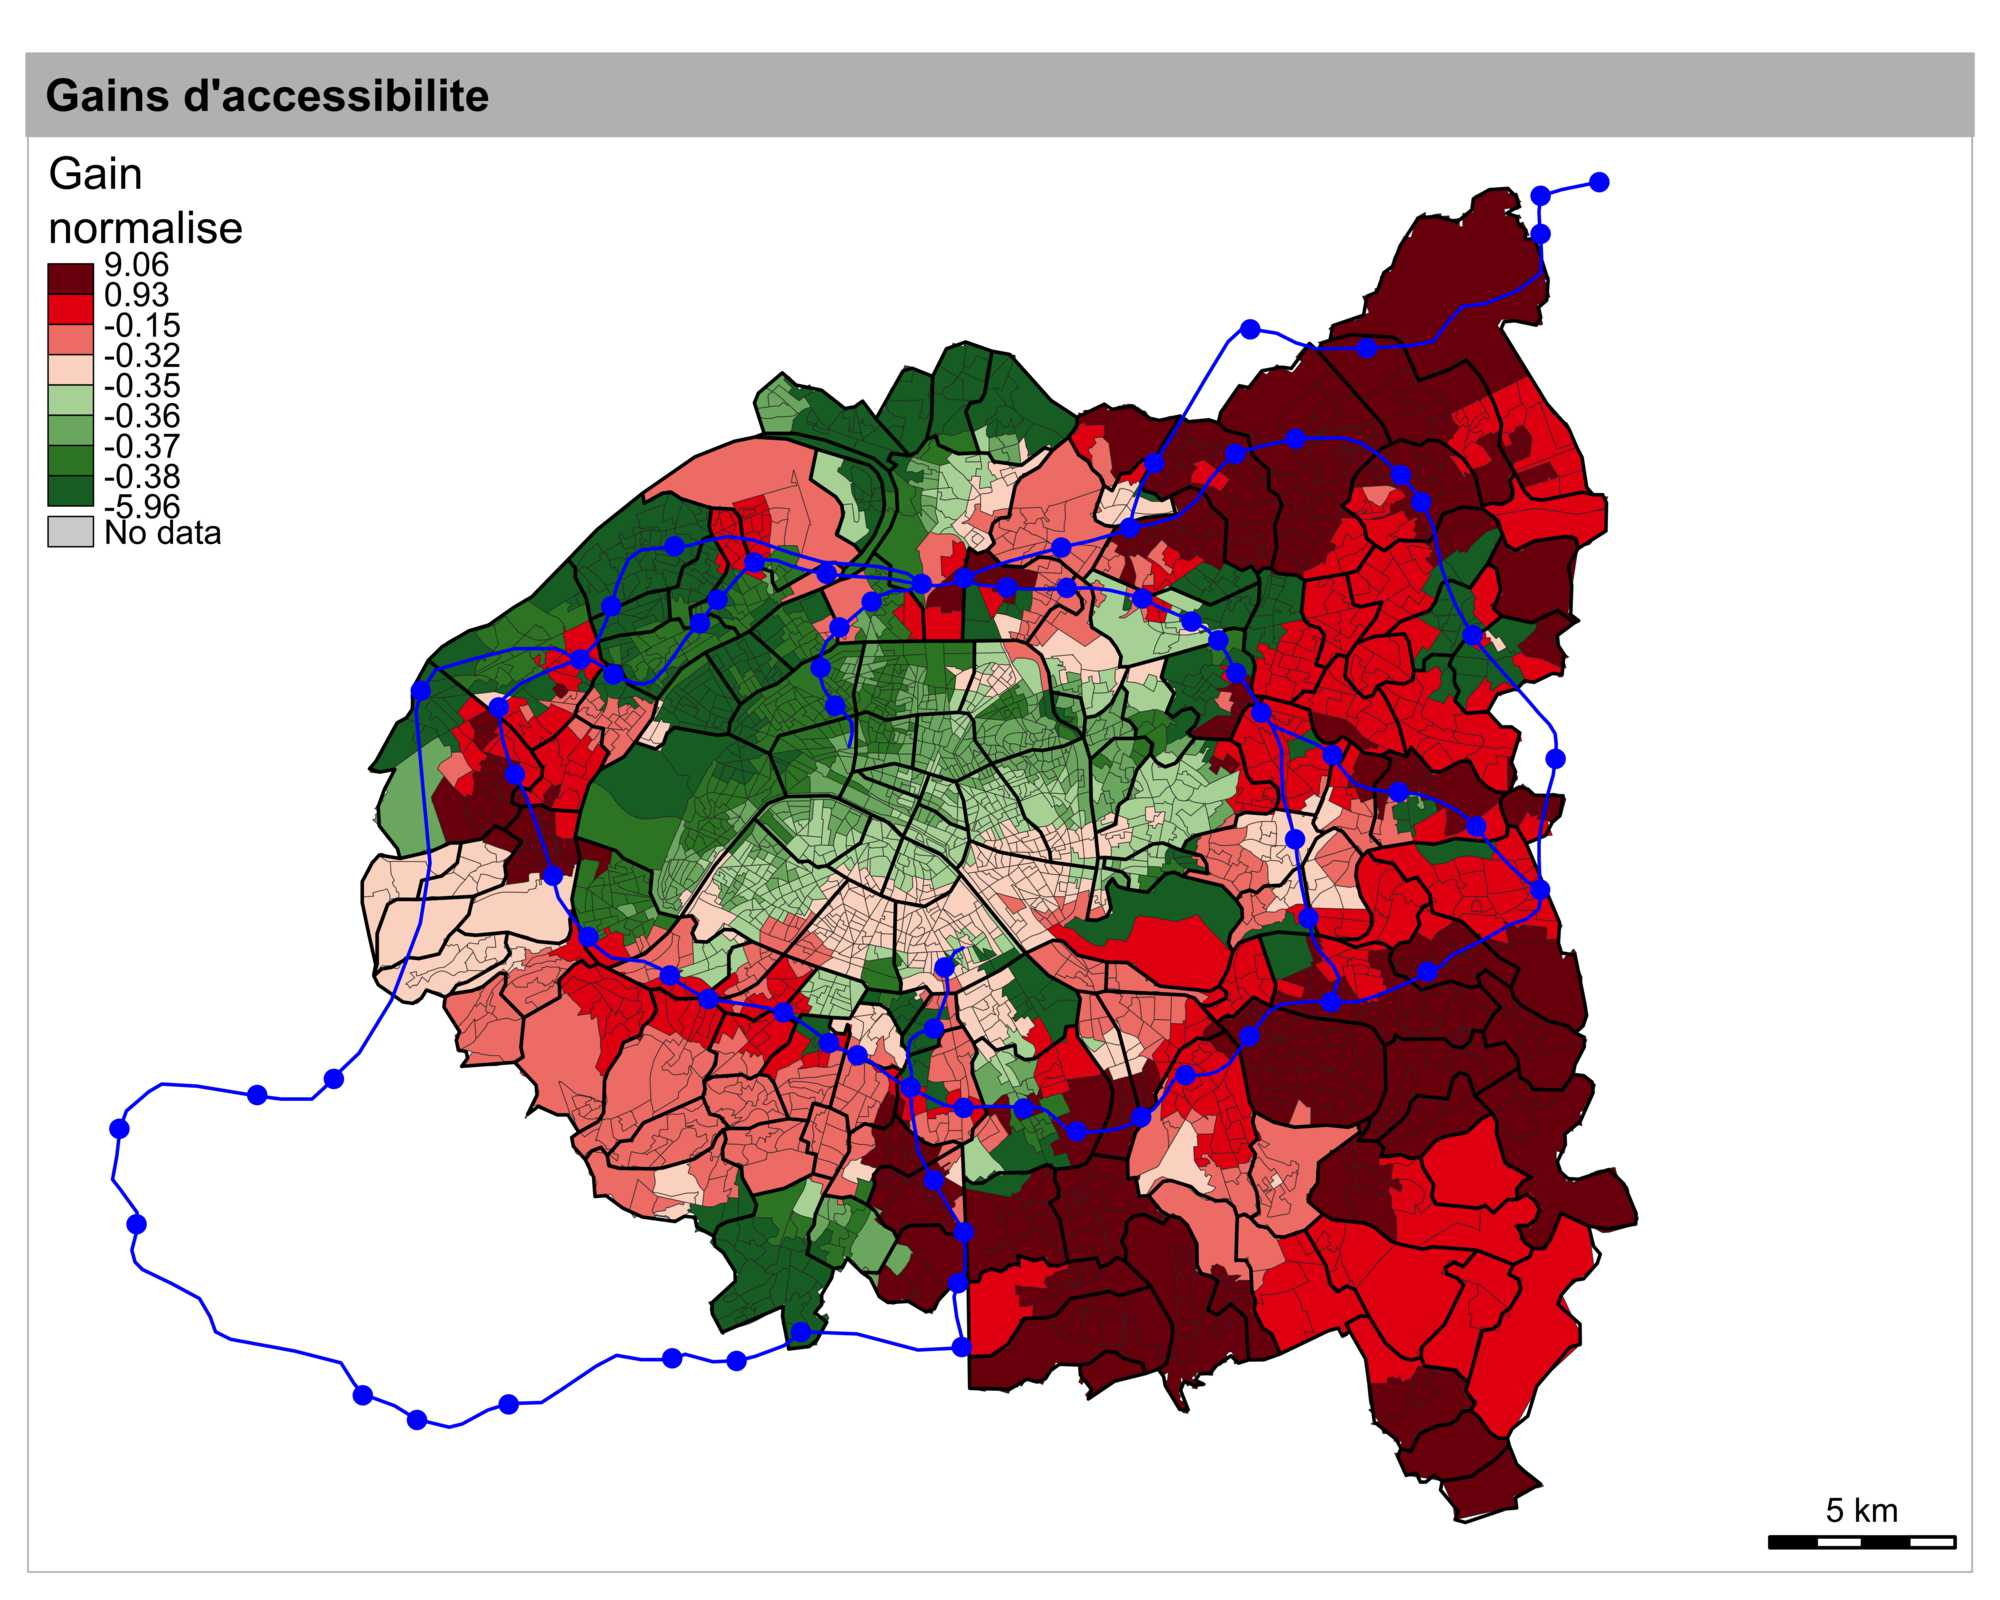
\includegraphics[width=0.8\textwidth]{figures/empirical-grdparis.jpg}
\end{center}	

	
	%\smallskip
	
	\footnotesize
	
	\vspace{-0.5cm}
	\begin{justify}
	\textit{Relations plus complexes dans le cas du gain d'accessibilité permis par le Grand Paris Express et les dynamiques socio-économiques des territoires}
	\end{justify}
	
	
%\end{column}
%\end{columns}

% LEGENDES

%\hspace{0.3cm}



}





%%%%%%%%%%%%%%%%%%%%%
\begin{frame}[allowframebreaks]
\frametitle{References}
\bibliographystyle{apalike}
\bibliography{biblio}
\end{frame}
%%%%%%%%%%%%%%%%%%%%%%%%%%%%







\end{document}







%%%%%
%% Below : slides de la reunion equipe -> select some as reserve slides



%\section*{Urban Morphogenesis}
% TODO Urban Morphogenesis



\sframe{Complex processes of Urban Morphogenesis}{

\centering

%% center of Paris
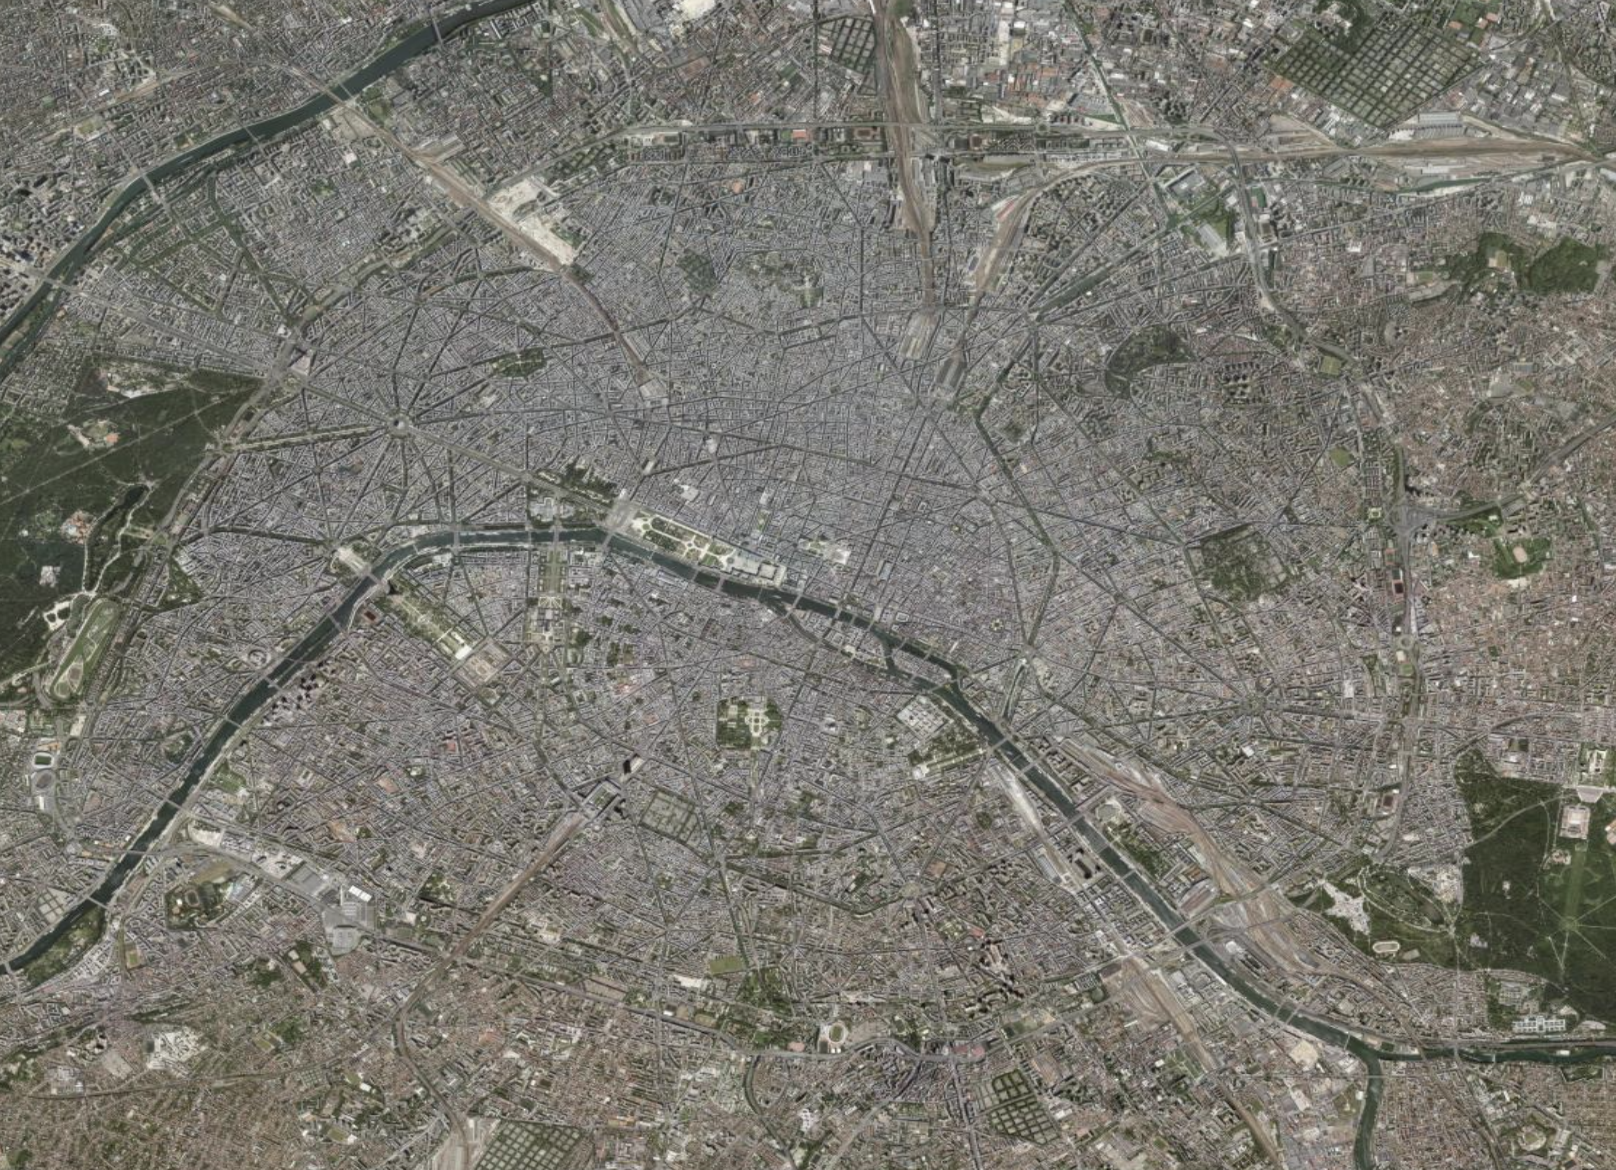
\includegraphics[width=0.9\textwidth]{figuresraw/intro_paname}

\footnotesize\textit{Source: Geoportail}
}

\sframe{Complex processes of Urban Morphogenesis}{

\centering

%% large bp
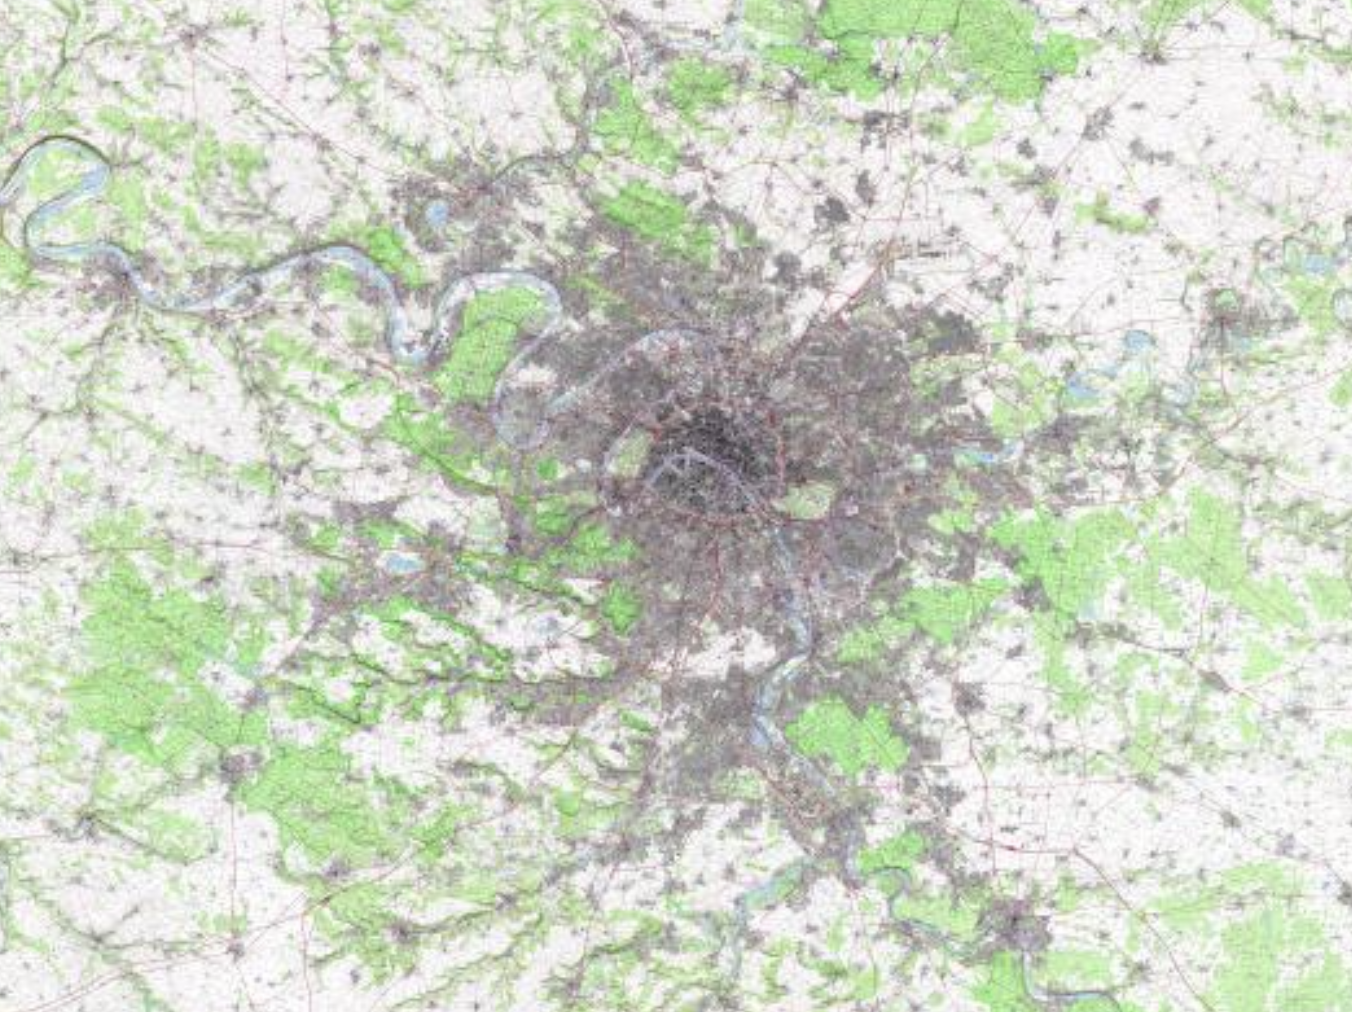
\includegraphics[width=0.9\textwidth]{figuresraw/intro_bp}

\footnotesize\textit{Source: Geoportail}
}




\sframe{What is Morphogenesis ?}{

\textbf{Morphogenesis} (\textit{Oxford dictionary}) 
\begin{enumerate}
\item \textit{Biology} : The origin and development of morphological characteristics
\item \textit{Geology} : The formation of landforms or other structures.
\end{enumerate}

\bigskip

\textbf{History of the notion}

$\rightarrow$ Started significantly with embryology around 1930~\cite{abercrombie1977concepts} 

$\rightarrow$ Turing's 1952 paper~\cite{turing1952chemical}, linked to the development of Cybernetics

$\rightarrow$ first use in 1871, large peak in usage between 1907-1909, increase until 1990, decrease until today. \textit{Scientific fashion ?}


}


%
%
%
%
%


\sframe{What is Morphogenesis ? Examples}{

%% illustrations : ants, geomorphology, neurons, self-assembly ; ARBOTRON ; paper nature aile avion
%% all from netlogo library ? would be nice illustration of generative nature
%
%
%% remark : do not put classical biological example to show how it has percolated to other fields


\vspace{-0.3cm}

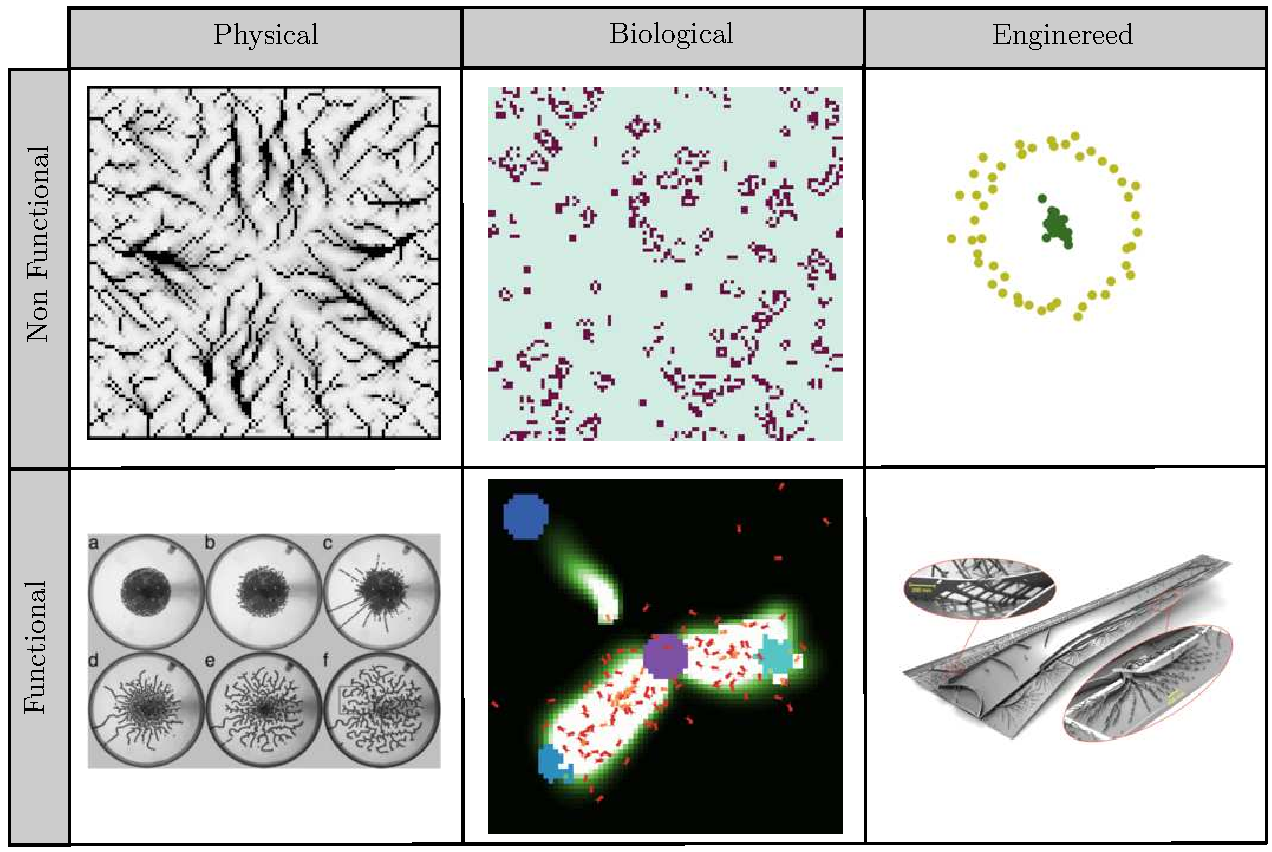
\includegraphics[width=\textwidth,height=0.82\textheight]{figuresraw/intro_examples.pdf}

\justify

\vspace{-0.5cm}

\footnotesize\textit{Sources (in order by column). Ants, Erosion, Game of Life: NetLogo Library ; Arbotron \cite{jun2005formation}; Industrial design \cite{Aage:2017aa}; Swarm chemistry \cite{sayama2007decentralized}}
%% sources : ants netlogo ; erosion netlogo ; arbotron 
%%  inge : 


}



%
%
%
\sframe{Defining Morphogenesis}{
%
%% precise notions and defs


\justify

\textit{Construction of an interdisciplinary definition : } %in~\cite{antelope2016interdisciplinary}}

\bigskip



\textbf{Meta-epistemological framework of imbricated notions:}

Self-organization $\supsetneq$ Morphogenesis $\supsetneq$ Autopoiesis $\supsetneq$ Life


\bigskip

\textbf{Properties:}

\begin{itemize}
\item Architecture links form and function
\item Emergence strength~\cite{bedau2002downward} increases with notion depth, as bifurcations~\cite{thom1974stabilite}
\end{itemize}

\bigskip

\textbf{Definition of Morphogenesis :} \textit{Emergence of the form and the function in a strongly coupled manner, producing an emergent architecture \cite{doursat2012morphogenetic}}


}





%
%
\sframe{Morphogenesis Overview}{

%% other numerous examples of fields/case of application

\cite{bourgine2010morphogenesis} : interdisciplinary workshop on morphogenesis

\bigskip

$\rightarrow$\textit{To what extent the notion is indeed transdisciplinary, i.e. are there common definitions across disciplines ? What are the concepts shared or the divergence ?}


\begin{itemize}
\item \textbf{Biology}
\begin{itemize}
\item External phenotype morphogenesis (ant colony)~\cite{minter2012morphogenesis} \item Symbiosis of species~\cite{chapman1998morphogenesis}
\item Botany~\cite{lord1981cleistogamy}
\end{itemize}
\item \textbf{Social Sciences} : Archeology~\cite{renfrew1978trajectory}
\item \textbf{Epistemology} : \cite{gilbert2003morphogenesis}
\item \textbf{Artificial Intelligence} : From self-assembly to Morphogenetic Engineering~\cite{doursat2013review}. Synthetic Biology ?
\item \textbf{Geomorphology} : dunes formation~\cite{douady2011dunes}
\item \textbf{Physics} : Arbotrons playing Tetris ?
\item etc\ldots
\end{itemize}




}



\sframe{Morphogenesis concepts}{

\begin{itemize}
\item \justify \textbf{Morphogenesis and Self-Organisation} : when does a system exhibit an architecture ? Insights from Morphogenetic Engineering
\cite{doursat2013review}. Architecture : the relation between the form and the function ?
\medskip
\end{itemize}
\begin{itemize}
\item \justify\textbf{Scales, Units and Boundaries} From local interactions to global information flow (Holland's \emph{signal and boundaries}~\cite{holland2012signals}: morphogenesis as the development of Complex Adaptive Systems ?)
\medskip
\end{itemize}
\begin{itemize}
\item \justify \textbf{Symmetry and Bifurcations} : on quantitative becoming qualitative. Ren{\'e} Thom's \emph{theory of catastrophes}~\cite{thom1974stabilite}
\medskip
\end{itemize}
\begin{itemize}
\item \justify \textbf{Life and Death} : link with autopoiesis and cognition\\
\cite{bourgine2004autopoiesis} ; co-evolution of subsystems as an alternative definition ? In psychology, attractors of the mind.
\end{itemize}


}


\sframe{Catastrophe Theory}{

%% brief rapide sur theorie des catastrophes

A system is viewed as its internal state $X_w$, where $w\in W$ is a control parameter.

\bigskip

Catastrophe set $K \subset W$ is where the system endures phase transition.

\bigskip

Thom classified possible topologies for $K$ depending on the dimension of $W$.

}



\sframe{Modeling Urban Morphogenesis}{

\justify

\cite{makse1998modeling} correlated growth; 

\cite{10.1371/journal.pone.0133780} multi-scale migration and percolation; 

\cite{bonin2012modele} qualitative differentiation of urban function; 

\cite{achibet2014model} procedural model at the micro-scale 

}






%
%

\sframe{Which models for Urban Morphogenesis ?}{

\justify

\begin{columns}
\column{0.4\textwidth}
\centering
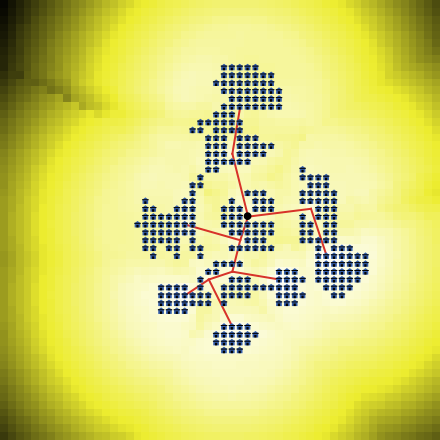
\includegraphics[width=\textwidth]{figuresraw/intro_RBD_lattice}\\
\footnotesize\textit{Example: a basic hybrid model based on elementary processes for density and network \cite{raimbault2014hybrid}}
\column{0.57\textwidth}
\justify

%%\vspace{-1cm}

$\rightarrow$\textit{At the crossroad between Urban Simulation and Artificial Life, few models try to integrate and explain the link between Urban Form and Function}

\medskip

$\rightarrow$\textit{Importance of parcimonious, stylized models: modeling as a tool to understand processes}

\end{columns}

\bigskip

\textbf{Research Objective : } Explore simple models to capture morphogenesis based on abstract representation of urban processes; test their ability to reproduce existing urban systems.



}



%%%%%
% here situation of urban/network morphogenesis models








\sframe{Different approaches to Network Morphogenesis}{

\vspace{-1cm}
\textit{Different models with different ontologies and coupling ontologies}

\bigskip
\bigskip

%\setlength{\columnseprule}{0.4pt}

\begin{columns}
\begin{column}{0.50\textwidth}
\centering\textit{Network}
\end{column}
%\vrule{}
%\vrule{}
\begin{column}{0.50\textwidth}
\centering\textit{Co-evolution}
\end{column}
\end{columns}

\bigskip

\begin{columns}
\begin{column}{0.25\textwidth}
\centering
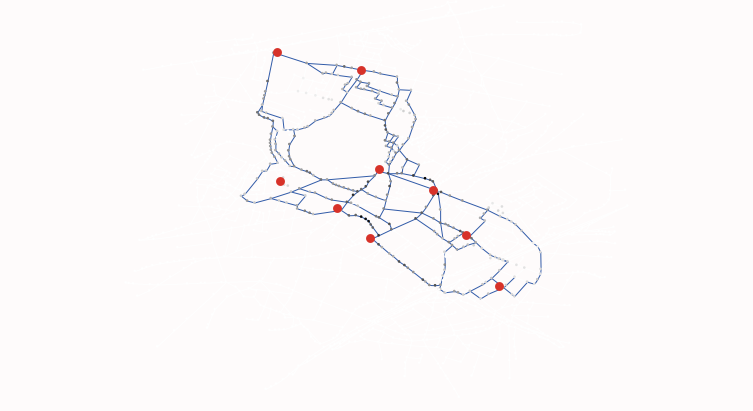
\includegraphics[width=\textwidth]{figuresraw/slimemould_reseauFinal}

\footnotesize\textit{Self-organizing biological network}

\medskip

\it\textbf{Optimisation}

\end{column}

\vspace*{-1cm}\vrule{}
\begin{column}{0.25\textwidth}
\centering
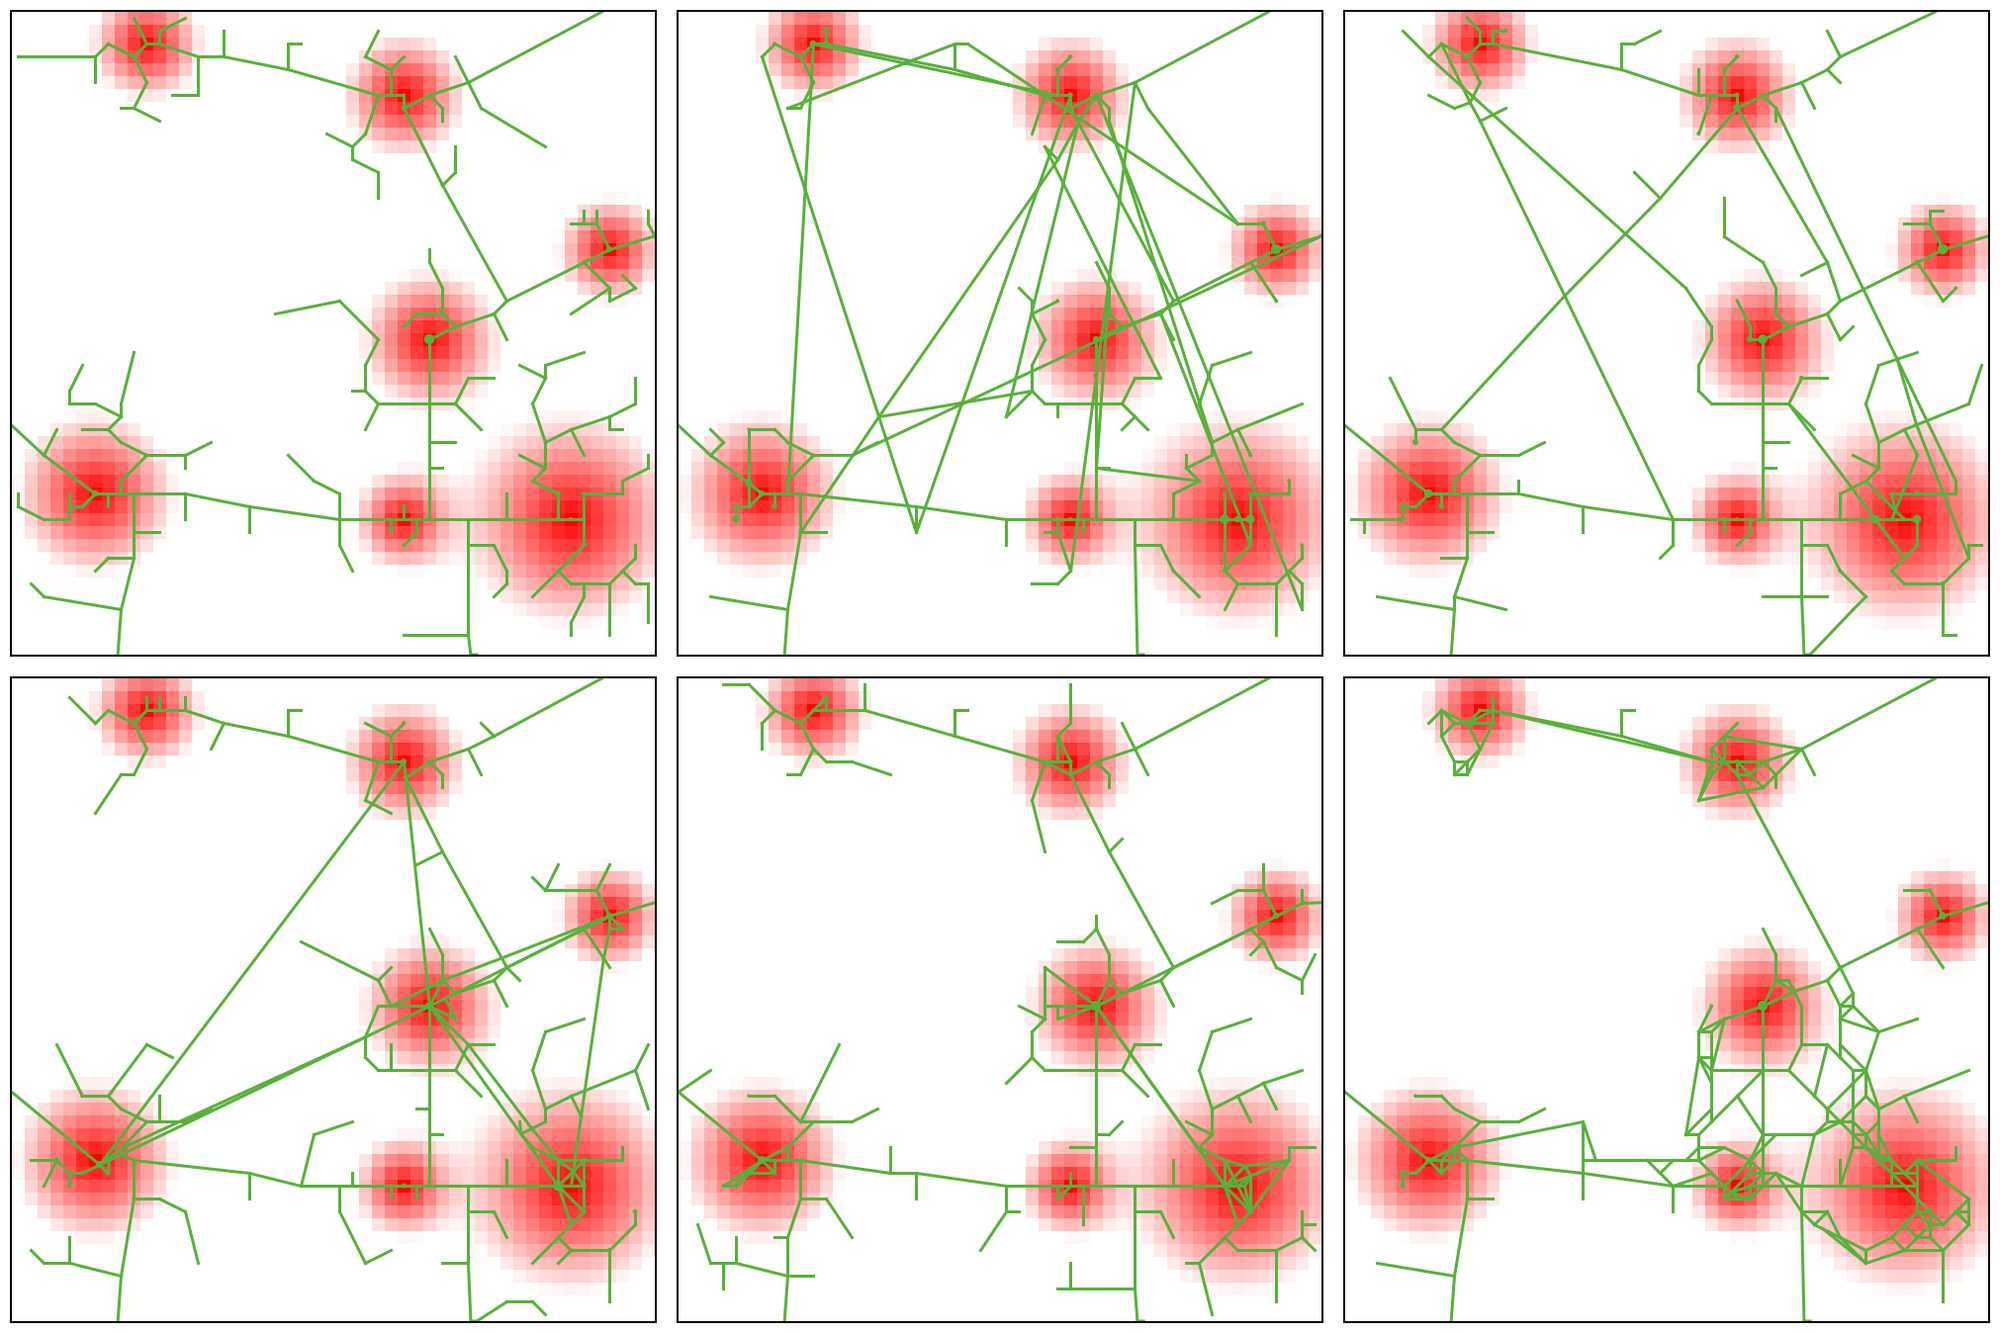
\includegraphics[width=\columnwidth]{../../Figures/Final/7-1-2-fig-networkgrowth-examples.jpg}

\footnotesize\textit{Multi-modeling network growth}
%
\medskip
%
\it\textbf{Explication}
\end{column}

\vrule{}
\begin{column}{0.25\textwidth}
\centering
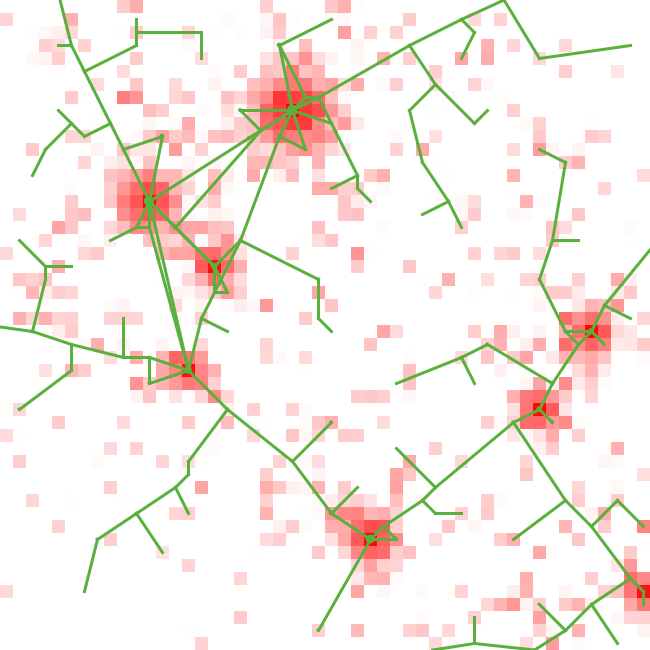
\includegraphics[width=\textwidth]{figuresraw/coevol_example_nw-cost}\\

\footnotesize\textit{Co-evolution model}

\medskip

\it\textbf{Explication}

\end{column}
\vrule{}
\begin{column}{0.25\textwidth}
\centering
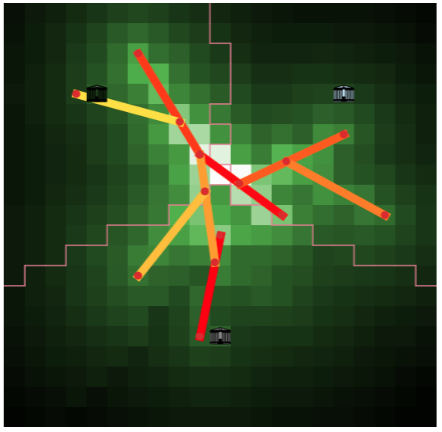
\includegraphics[width=\textwidth]{figuresraw/lutetia_longtimelimit_2.png}\\

\footnotesize\textit{Transportation governance}

\medskip

\it\textbf{Explication}

\end{column}
\end{columns}

%\setlength{\columnseprule}{0pt}

}






\sframe{Different models of Urban Morphogenesis}{

\vspace{-1cm}
\textit{Four different models with different ontologies and coupling ontologies}

\bigskip
\bigskip

%\setlength{\columnseprule}{0.4pt}

\begin{columns}
\begin{column}{0.25\textwidth}
\centering\textit{Network}
\end{column}
%\vrule{}
\begin{column}{0.25\textwidth}
\centering\textit{Density}
\end{column}
%\vrule{}
\begin{column}{0.50\textwidth}
\centering\textit{Co-evolution}
\end{column}
\end{columns}

\bigskip

\begin{columns}
\begin{column}{0.25\textwidth}
\centering
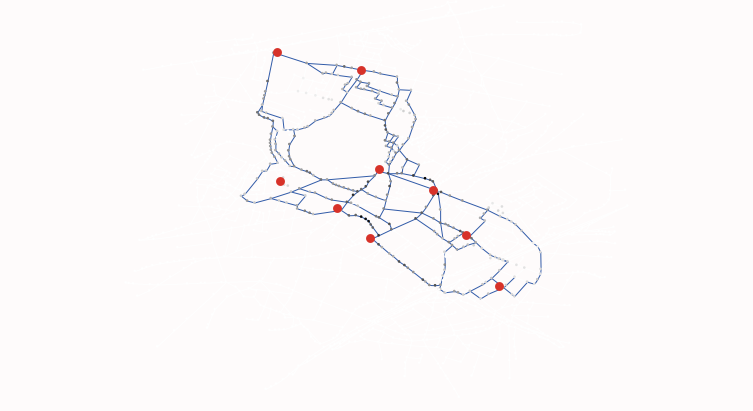
\includegraphics[width=\textwidth]{figuresraw/slimemould_reseauFinal}

\footnotesize\textit{Self-organizing network}

\medskip

\it\textbf{Optimisation}

\end{column}
\vspace*{-1cm}\vrule{}
\begin{column}{0.25\textwidth}
\centering
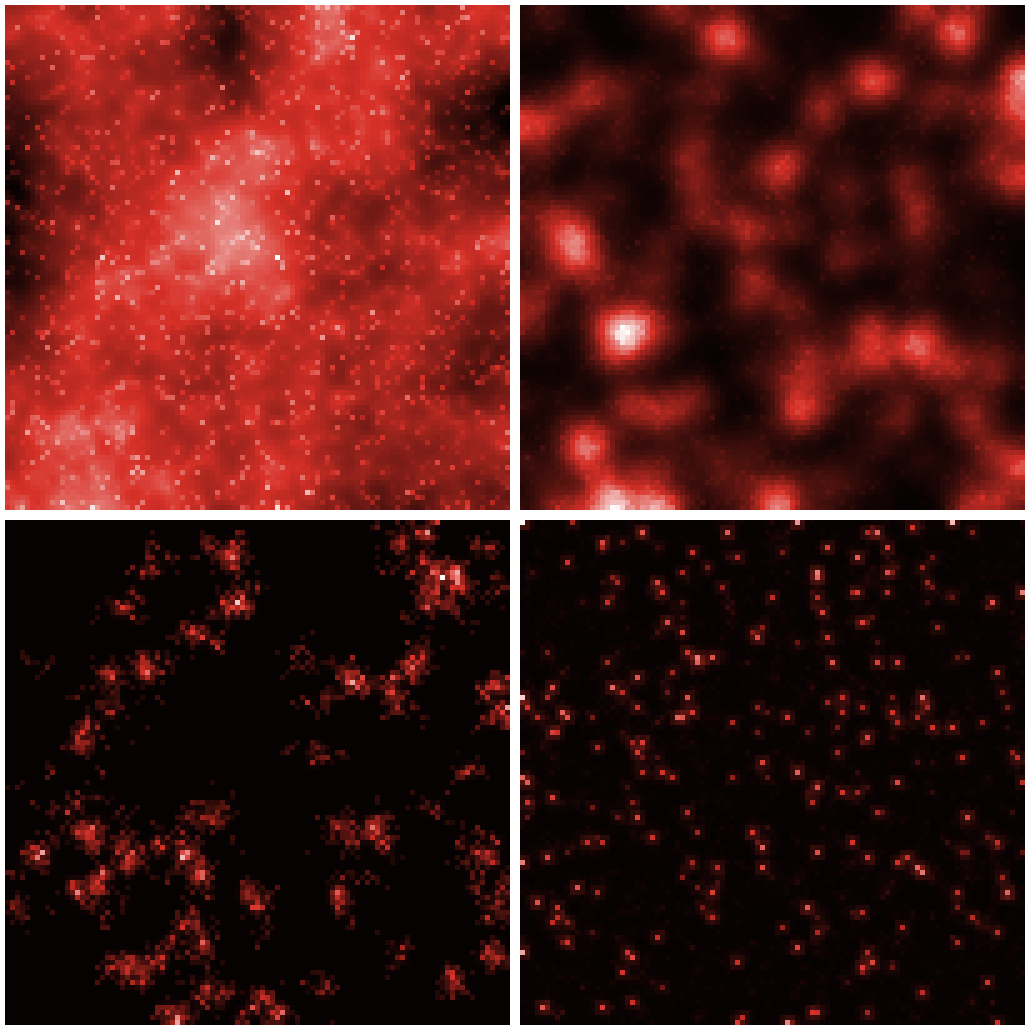
\includegraphics[width=\textwidth]{figuresraw/density_Fig2}

\footnotesize\textit{Reaction-diffusion density-based model}

\medskip

\it\textbf{Explication}
\end{column}
\vspace*{-1cm}\vrule{}
\begin{column}{0.25\textwidth}
\centering
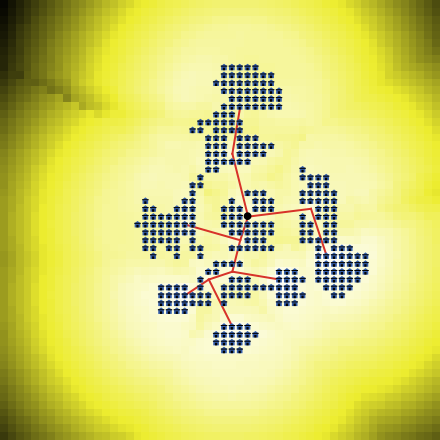
\includegraphics[width=\textwidth]{figuresraw/intro_RBD_lattice}\\

\footnotesize\textit{Basic hybrid model}\\\cite{raimbault2014hybrid}

\medskip

\it\textbf{Optimisation}
\end{column}
\vrule{}
\begin{column}{0.25\textwidth}
\centering
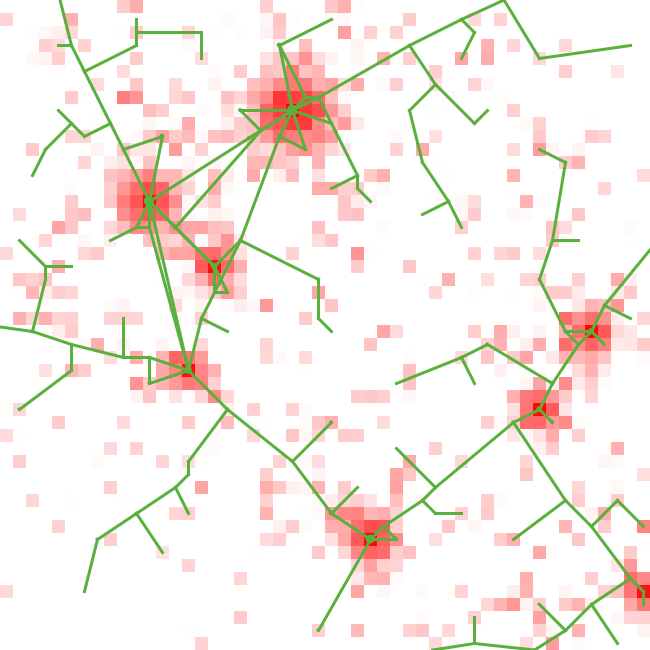
\includegraphics[width=\textwidth]{figuresraw/coevol_example_nw-cost}\\

\footnotesize\textit{Co-evolution model}

\medskip

\it\textbf{Explication}

\end{column}
\end{columns}

%\setlength{\columnseprule}{0pt}

}












%\section*{Reaction-diffusion model}
% TODO Reaction-diffusion model


\sframe{A simple Reaction-diffusion model}{
%
%% comment Arnaud : reaction-diffusion ?
%
%% model rationale and processes

\justify

$\rightarrow$ Crucial role of the interplay between concentration forces and dispersion forces~\cite{fujita1996economics} in keeping Urban Systems at the border of chaos

\bigskip

$\rightarrow$ Potentiality of aggregation mechanisms (such as Simon model) to produce power laws \cite{2016arXiv160806313S}

\bigskip

$\rightarrow$ Link with Reaction-diffusion approaches in Morphogenesis~\cite{turing1952chemical}

\bigskip

$\rightarrow$ Extension of a DLA-type model introduced by \cite{batty1991generating}, with simple abstract processes of population aggregation and diffusion

}



\sframe{Model Formalization}{

%% model formalization and indicators

$\rightarrow$ Grid world with cell populations $(P_i(t))_{1\leq i\leq N^2}$.

\bigskip

$\rightarrow$ At each time step:



\begin{enumerate}
\item Population growth with exogenous rate $N_G$, attributed independently to a cell following a preferential attachment of strength $\alpha$
%%\begin{equation}
%%\Pb{P_i(t+1)=P_i(t)+1|P(t+1)=P(t)+1}=\frac{(P_i(t)/P(t))^{\alpha}}{\sum(P_i(t)/P(t))^{\alpha}}
%%\end{equation}
%%The attribution being uniformly drawn if all population are equal to 0.
\item Population is diffused $n_d$ times with strength $\beta$
\end{enumerate}

\bigskip

$\rightarrow$ Stopping criterion: fixed maximal population $P_m$.

%%To avoid bord effects such as reflecting diffusion waves, border cells diffuse their due proportion outside of the world, implying that the total population at time $t$ is strictly smaller than $N_G\cdot t$.

\bigskip

$\rightarrow$ Output measured by morphological indicators: Moran index, average distance, rank-size hierarchy, entropy.


}



%
%
\sframe{Generating Population Distributions}{
%
%
%% examples : fig 2 of paper
%


\centering

\includegraphics[height=0.8\textheight]{../../Figures/Final/5-2-2-fig-density-fig2.jpg}

%


\footnotesize\textit{Examples of generated territorial shapes}

}


%
%


\sframe{Model behavior}{

\centering

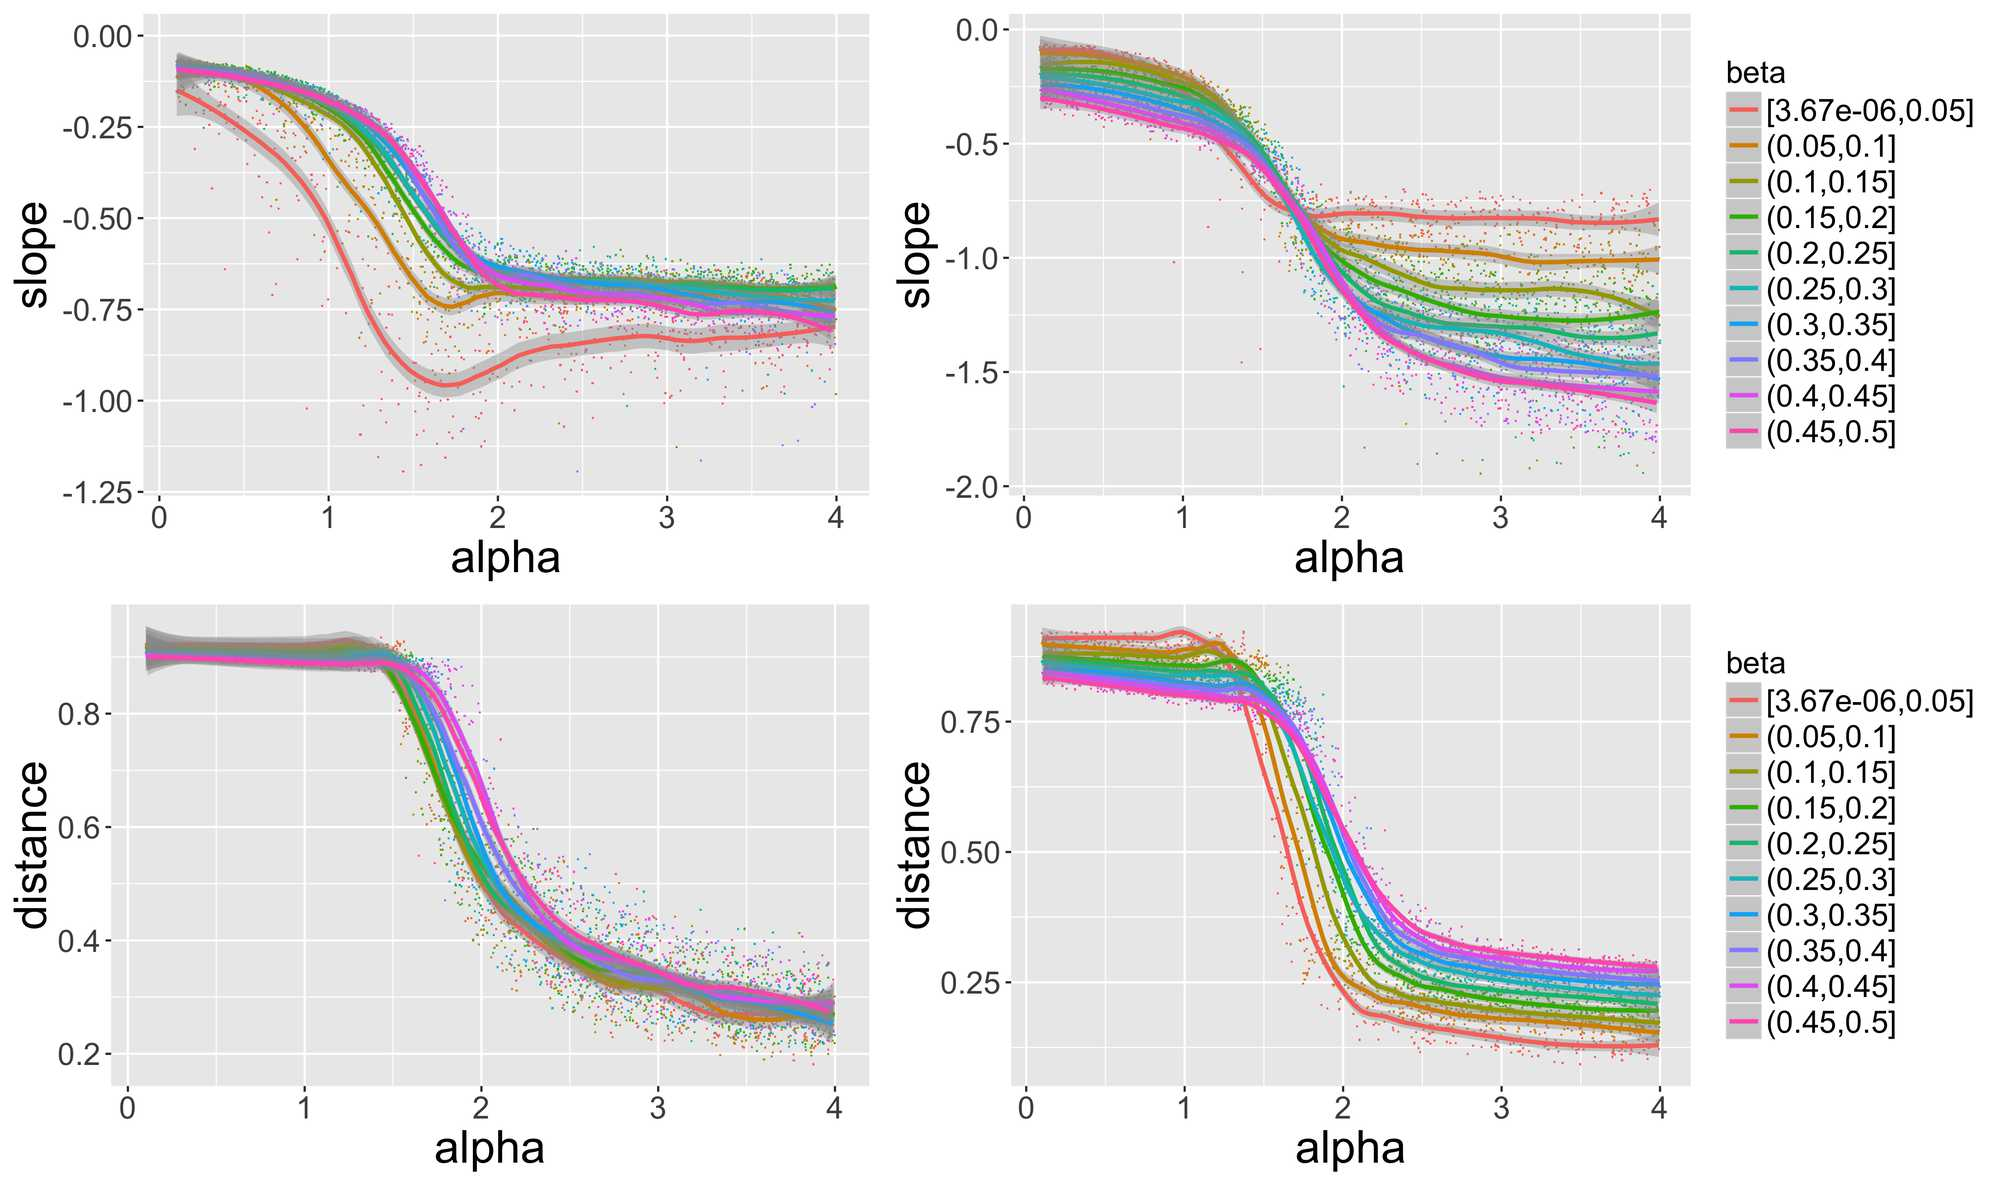
\includegraphics[width=0.9\textwidth]{../../Figures/Final/5-2-2-fig-density-fig3.jpg}

\footnotesize\textit{Phase transitions of indicators unveiled by exploration of the parameter space (80000 parameter points, 10 repetitions each)}

}



%
%
%
%
%


\sframe{Path-dependence and frozen accidents}{

\centering

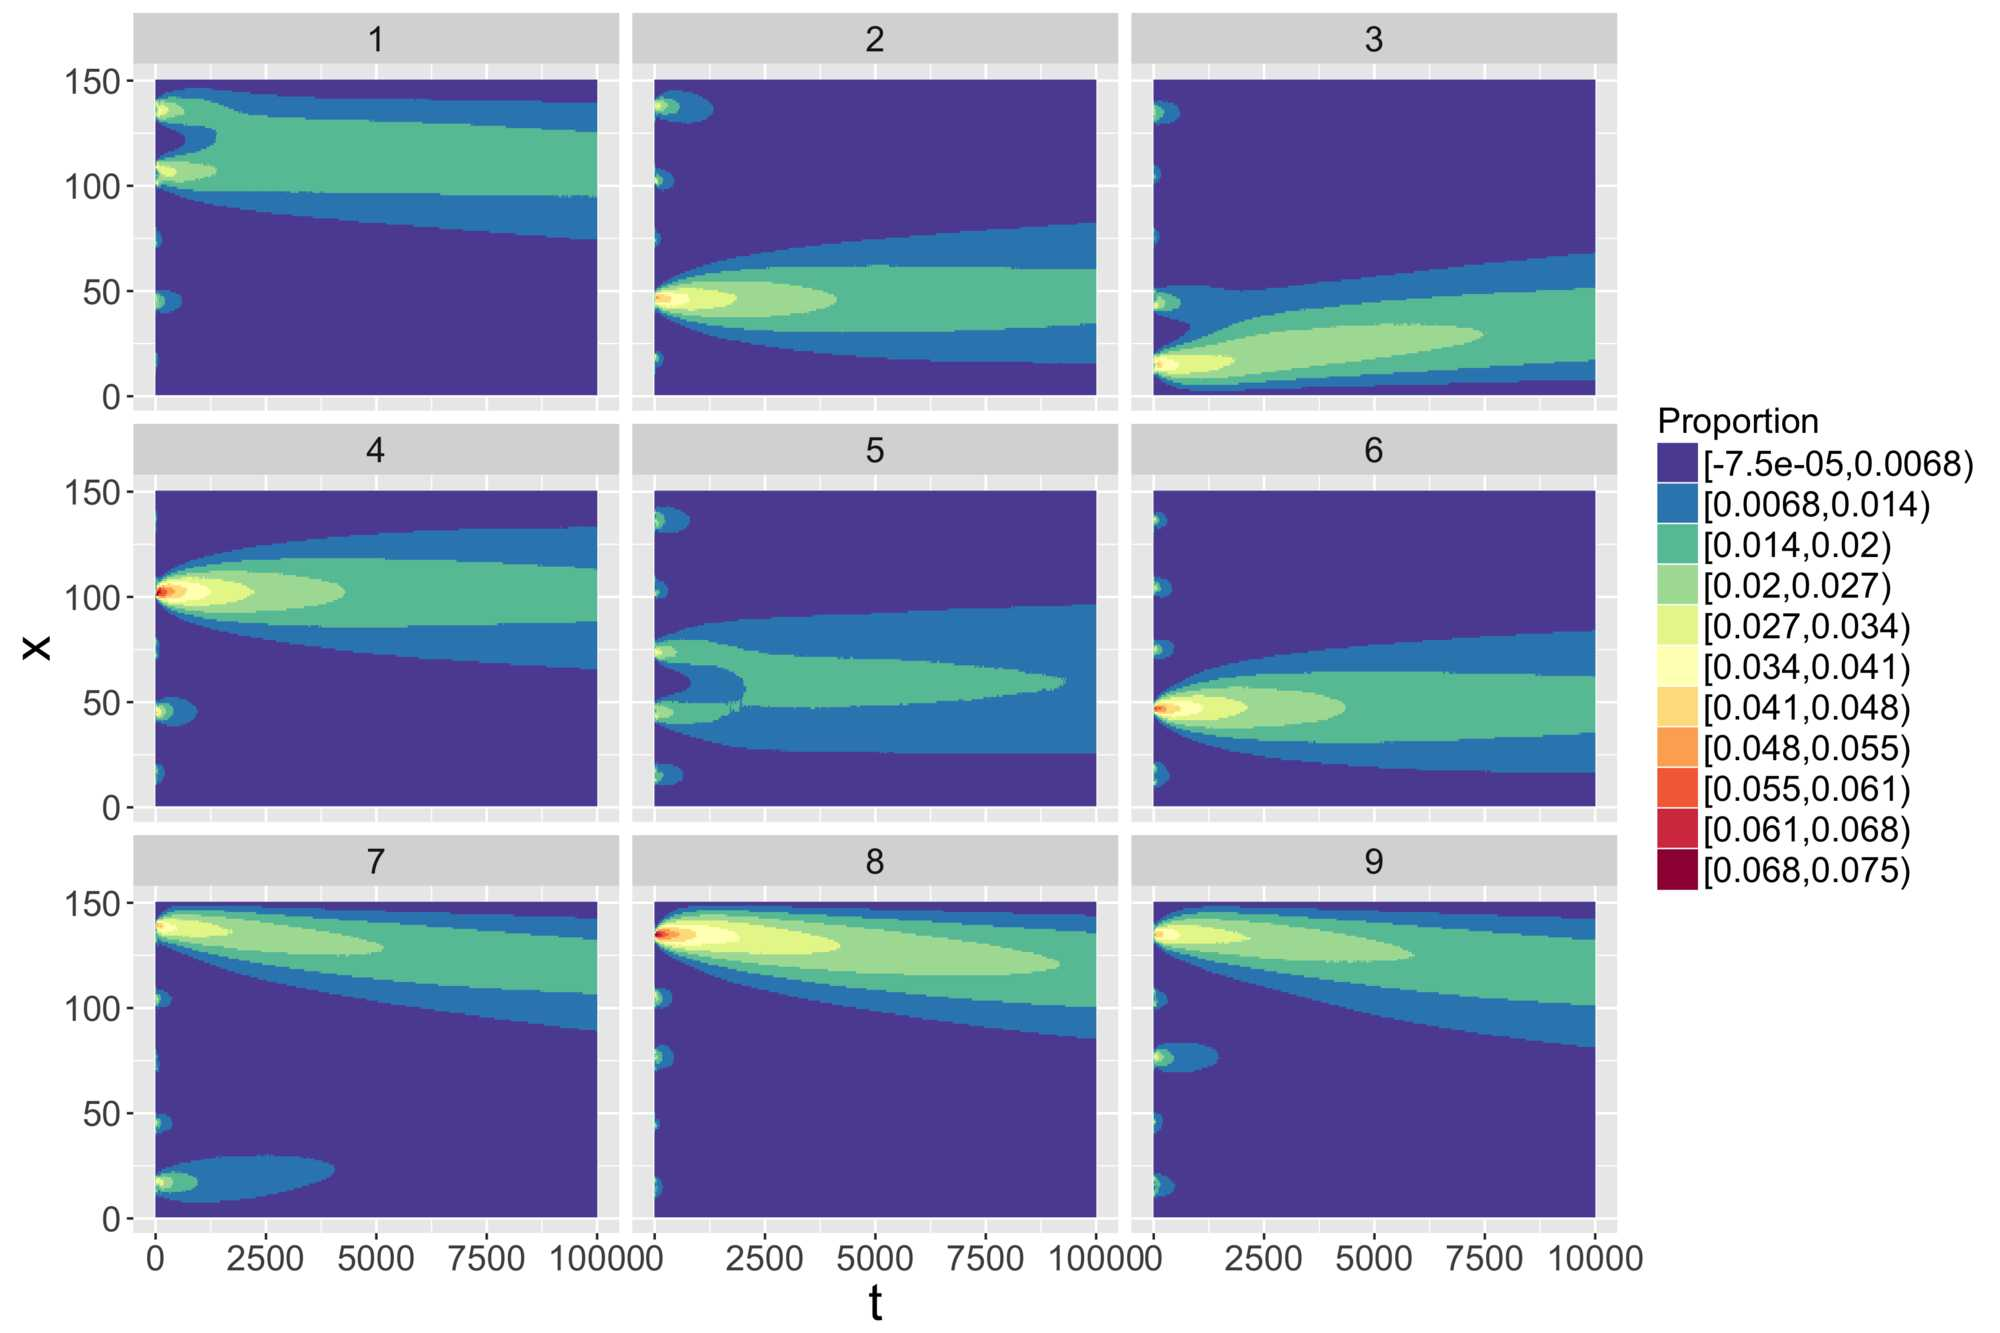
\includegraphics[width=0.8\textwidth]{../../Figures/Final/5-2-2-fig-density-fig4.jpg}

\footnotesize\textit{Illustration of path-dependence in a simplified one-dimensional version of the model: cell trajectories in time for 9 independent repetitions from the same initial configuration.}


}



%

\sframe{Empirical Data for Calibration}{
%

\begin{columns}
\column{0.6\textwidth}
\centering

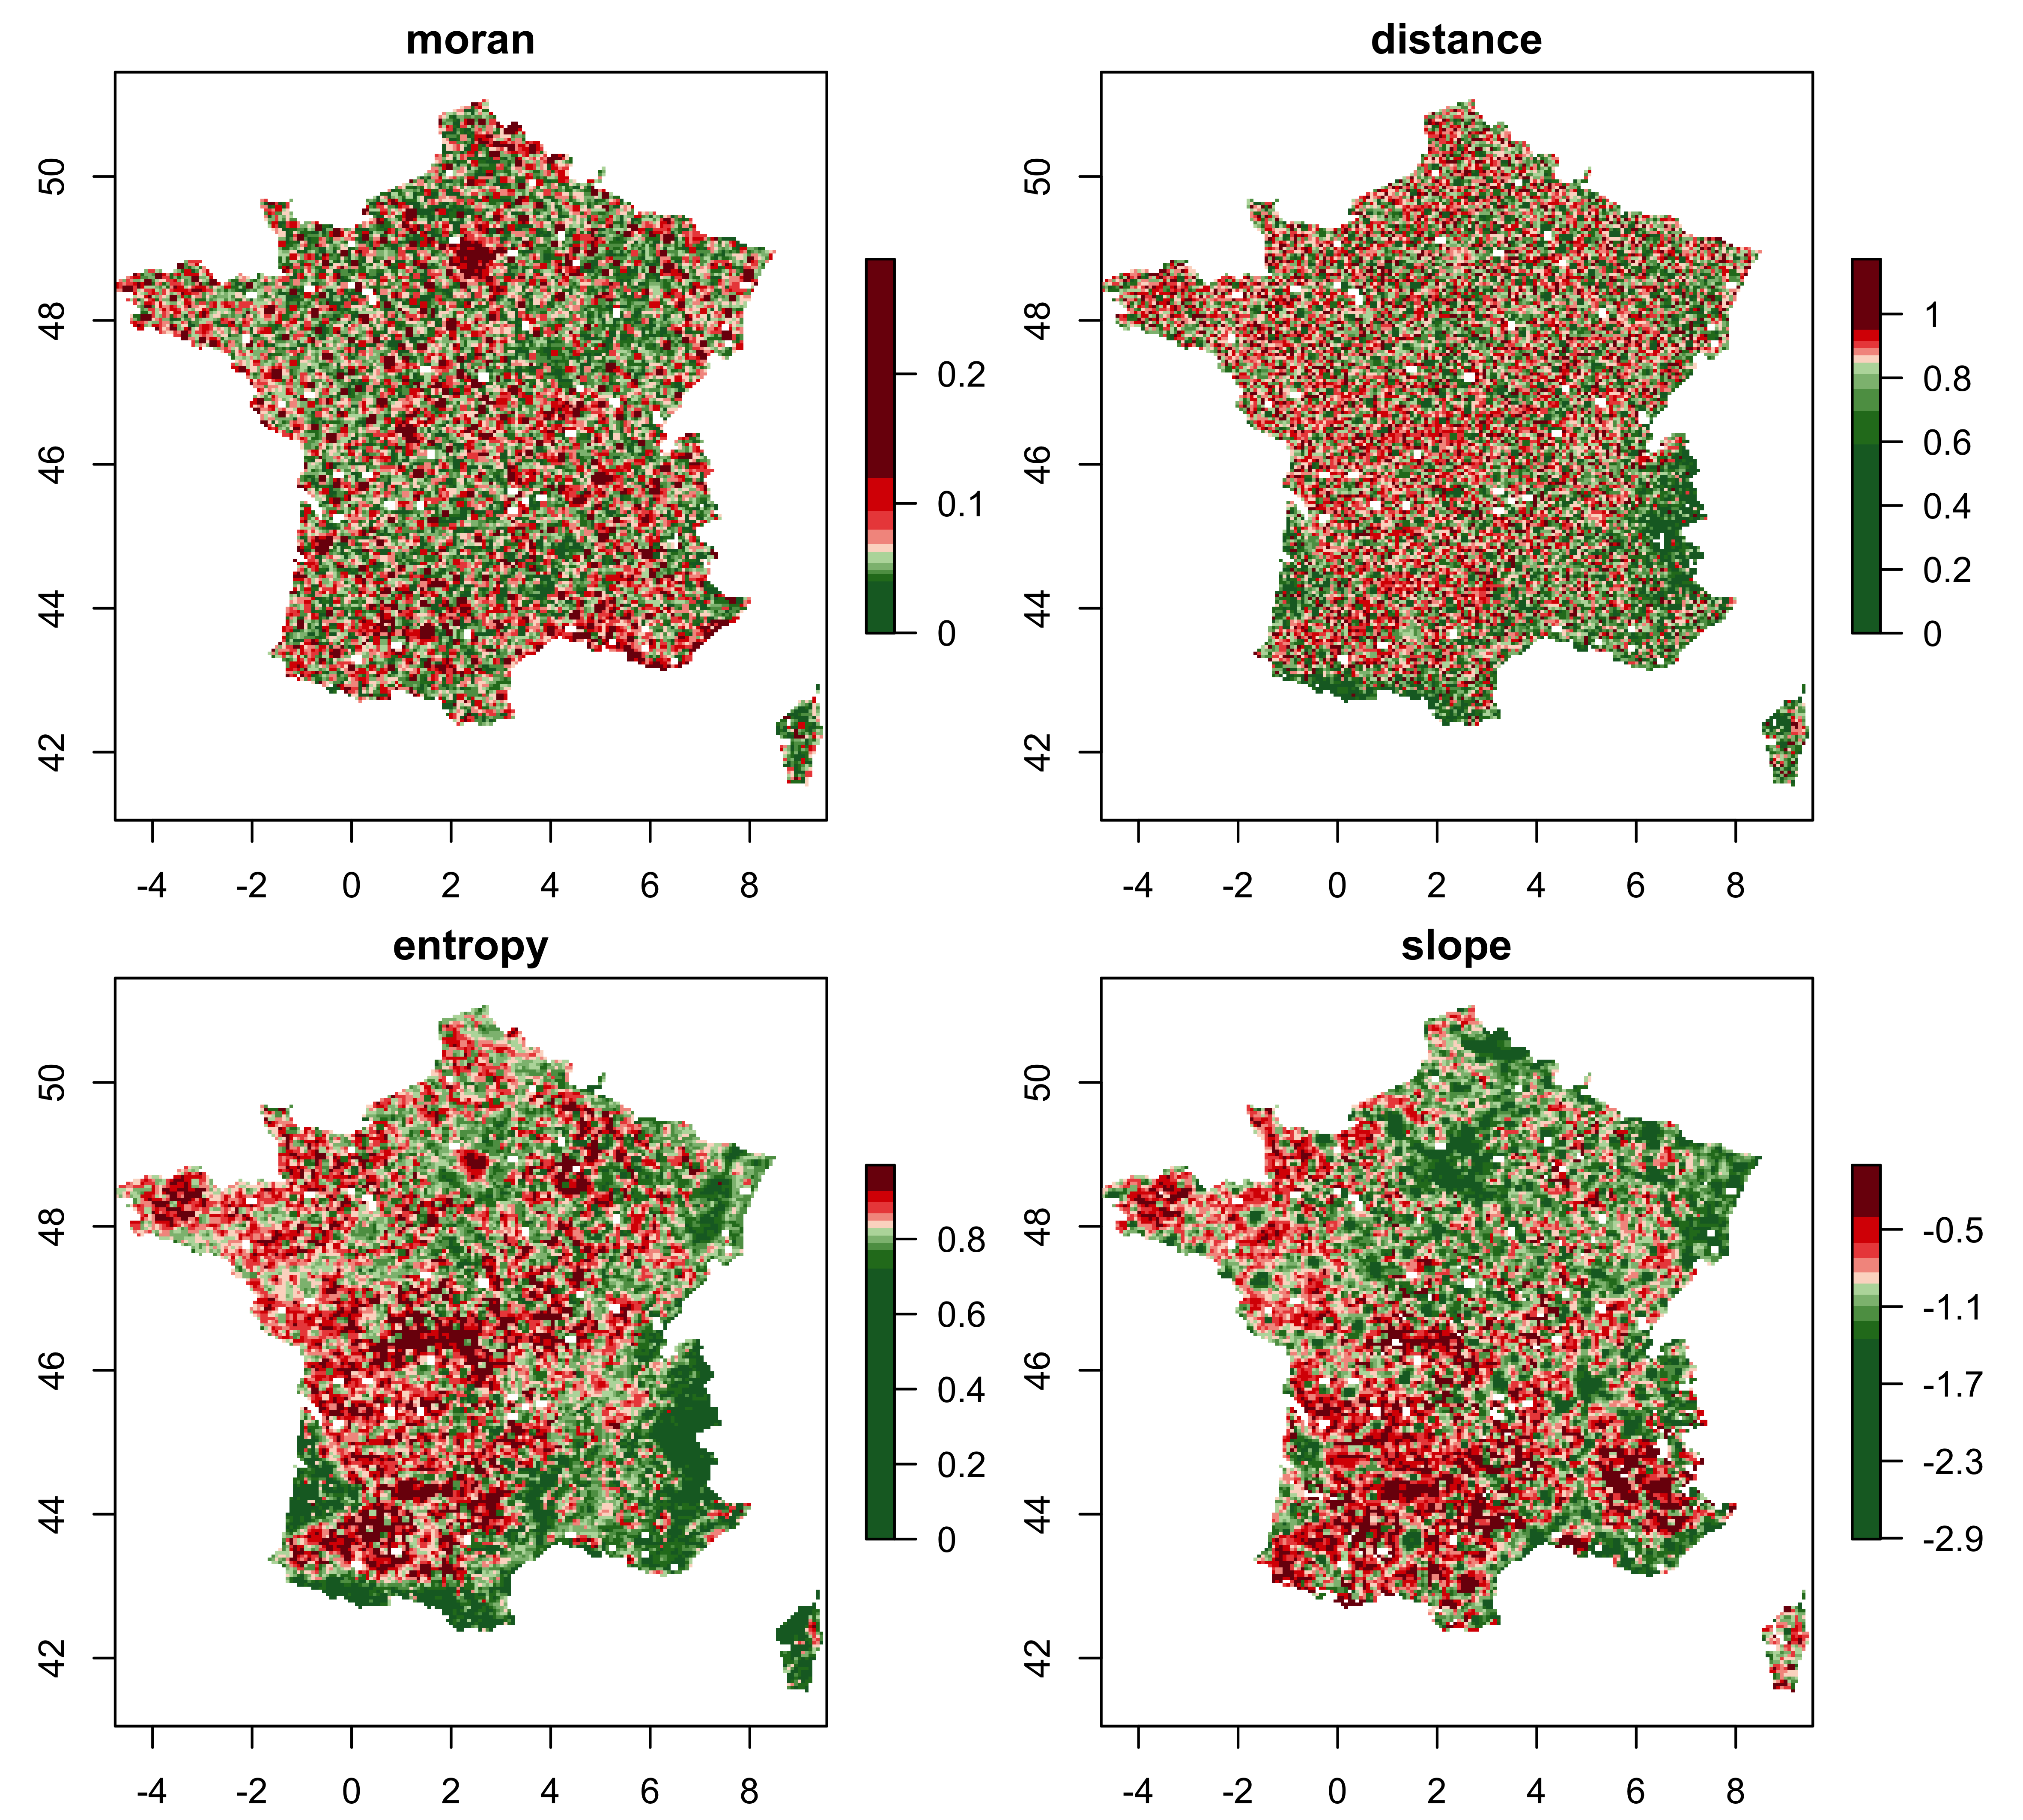
\includegraphics[width=\textwidth]{figuresraw/density_indics_morpho_discrquantiles}

\column{0.3\textwidth}
\centering

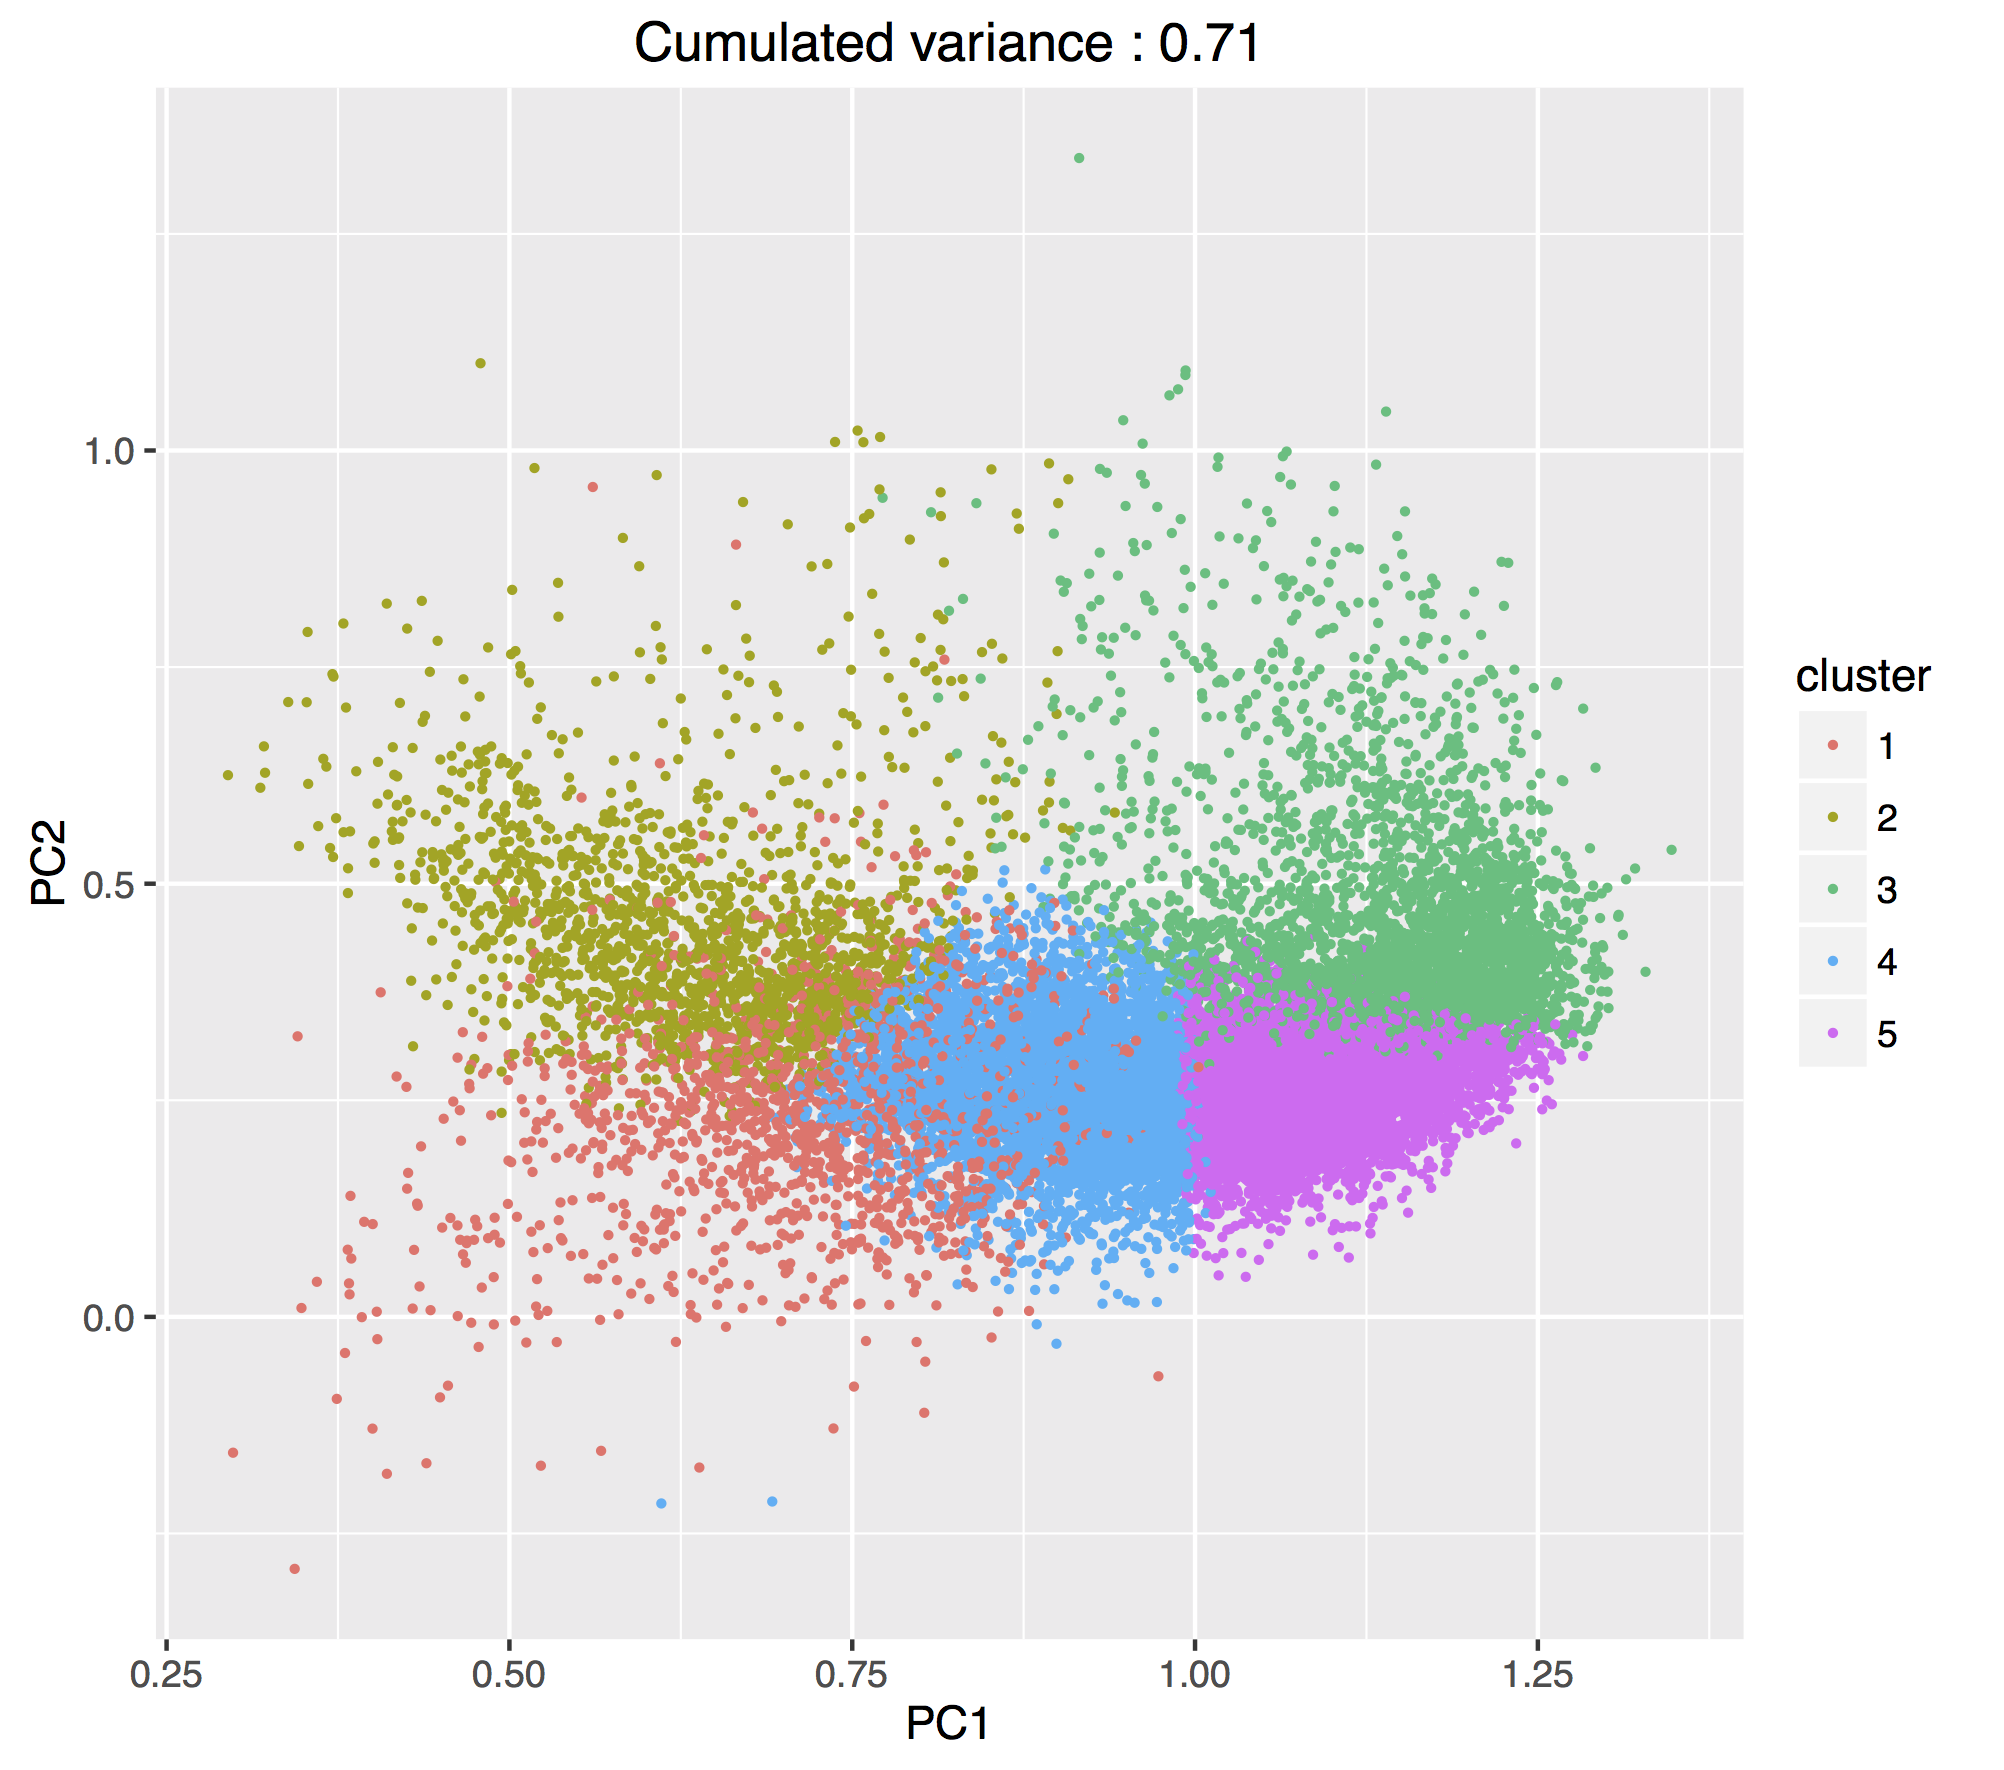
\includegraphics[width=\textwidth]{figuresraw/density_cluster_pca_k5_morpho}\\
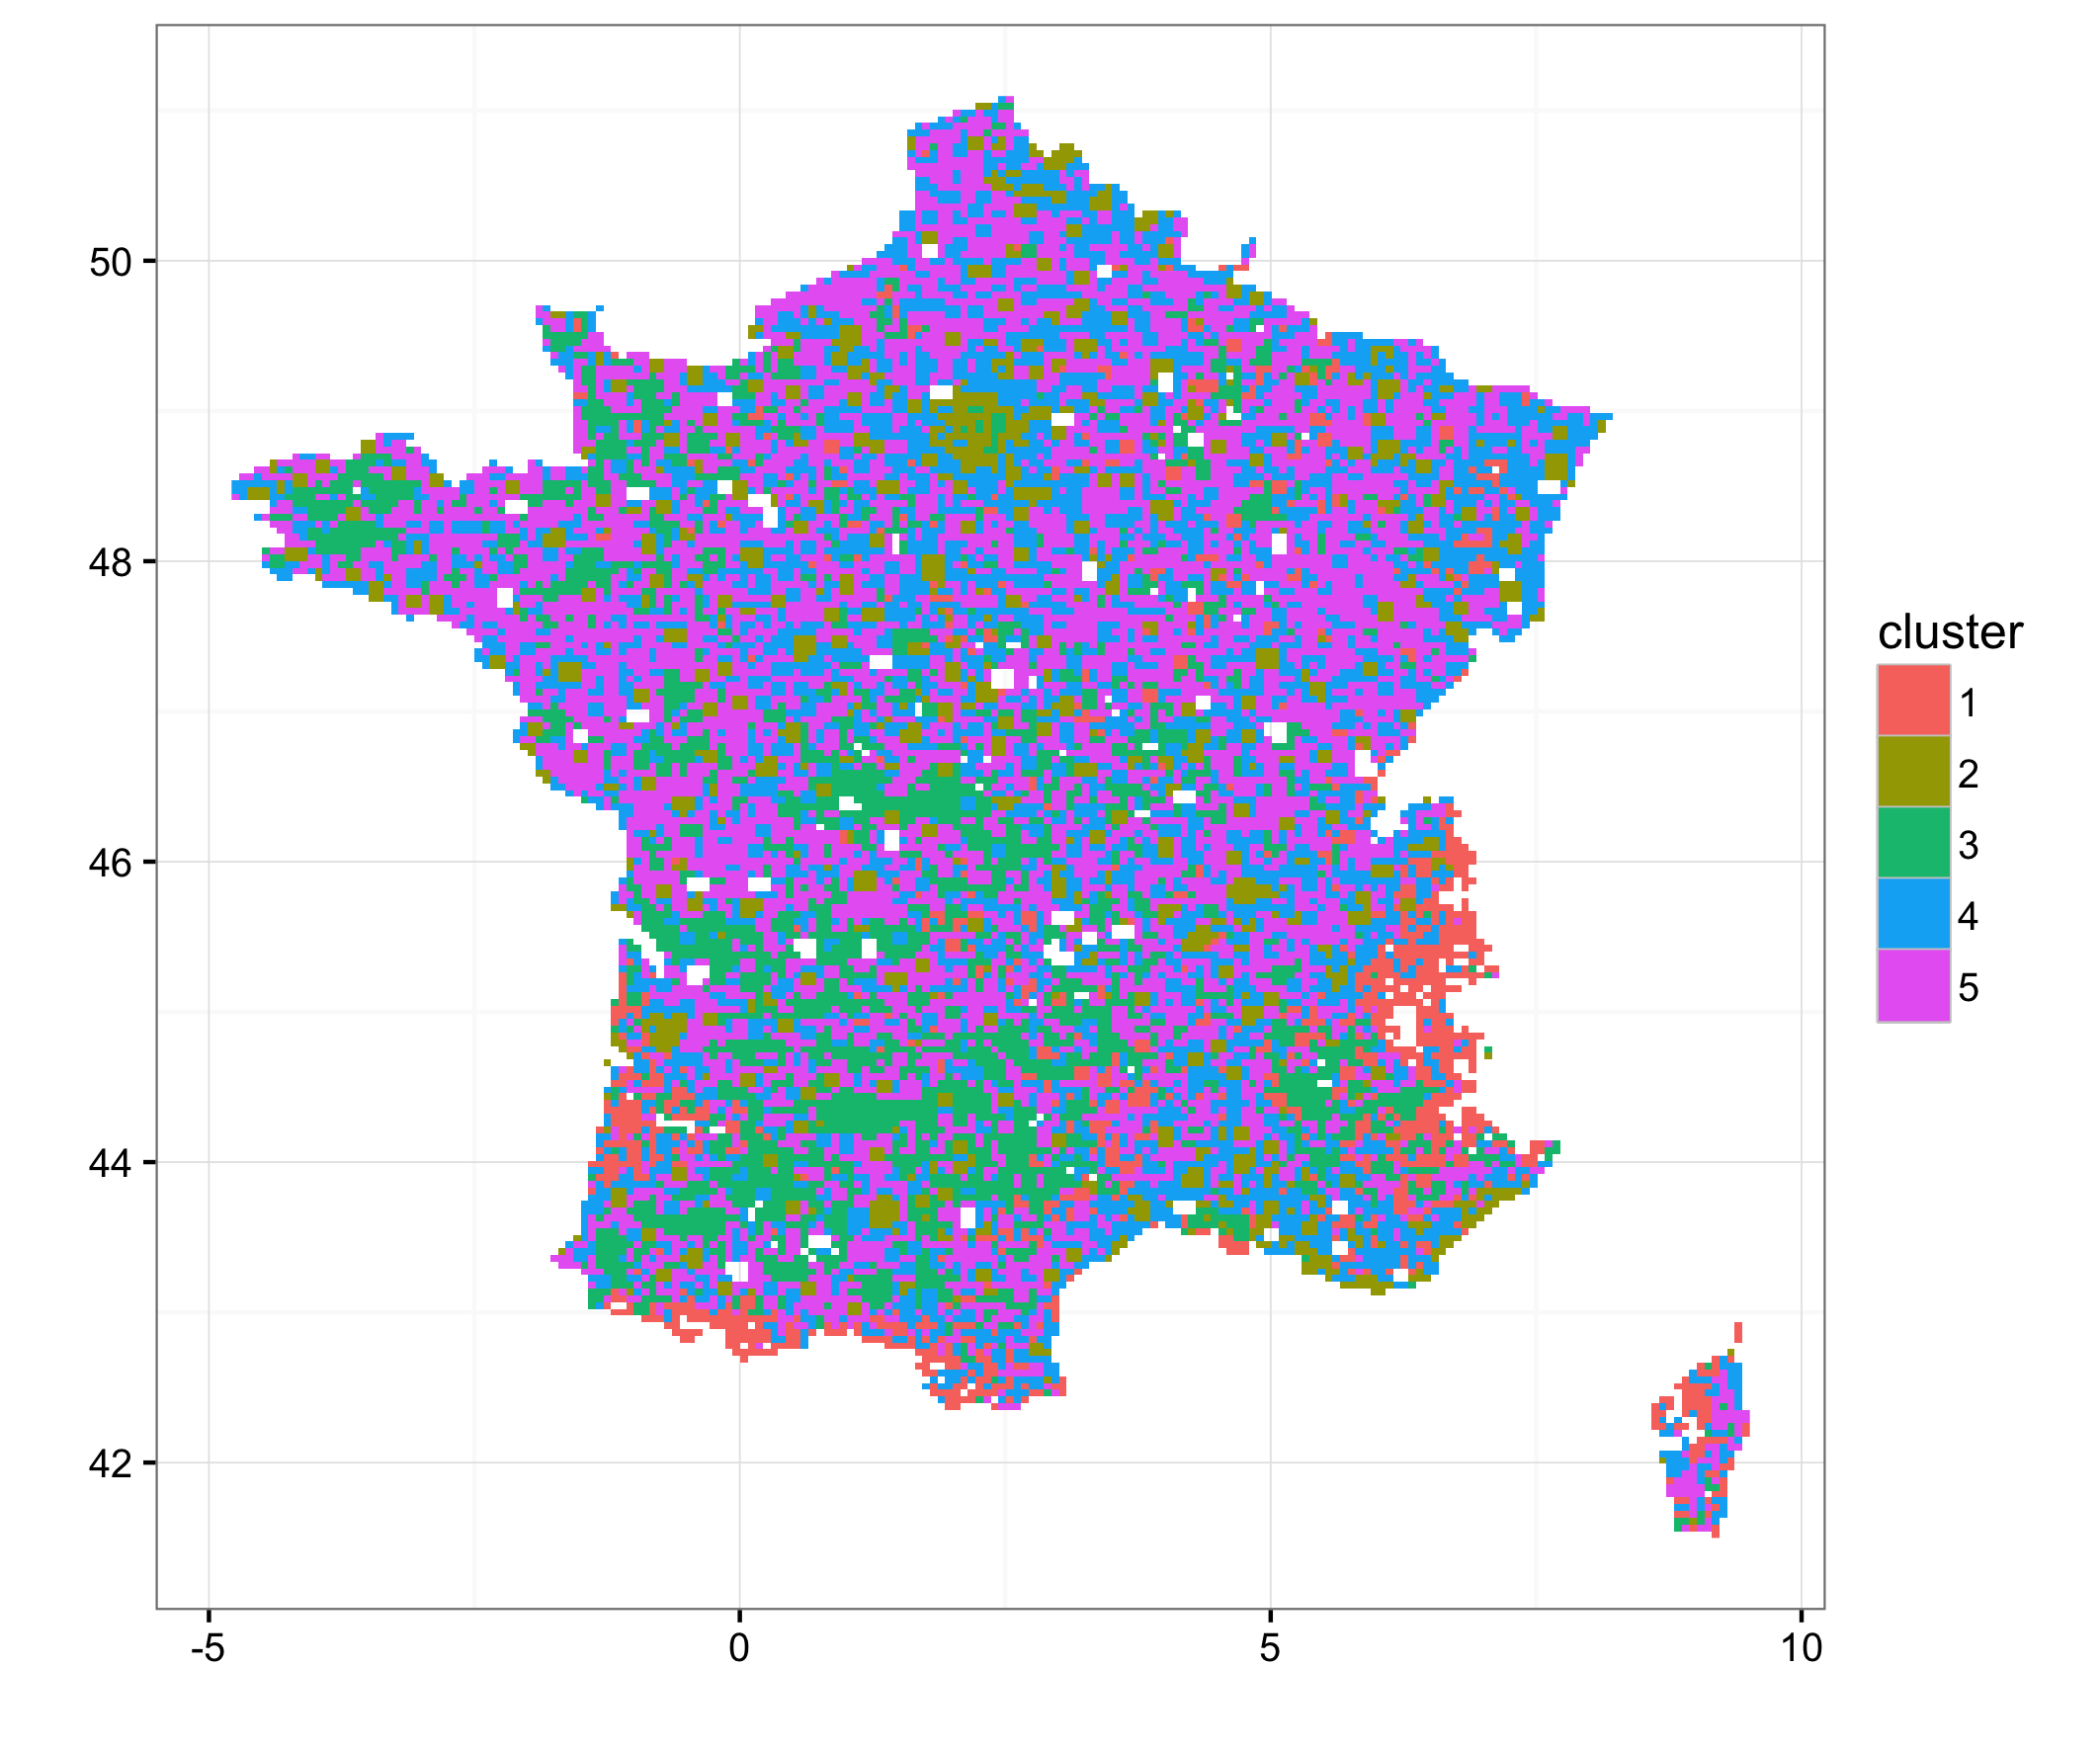
\includegraphics[width=\textwidth]{figuresraw/density_cluster_map_k5_morpho}

\end{columns}

\justify

\footnotesize\textit{Computation of morphological indicators on population density data for Europe (shown here on France), morphological classification.}

}


%
%
%


\sframe{Model Calibration}{

%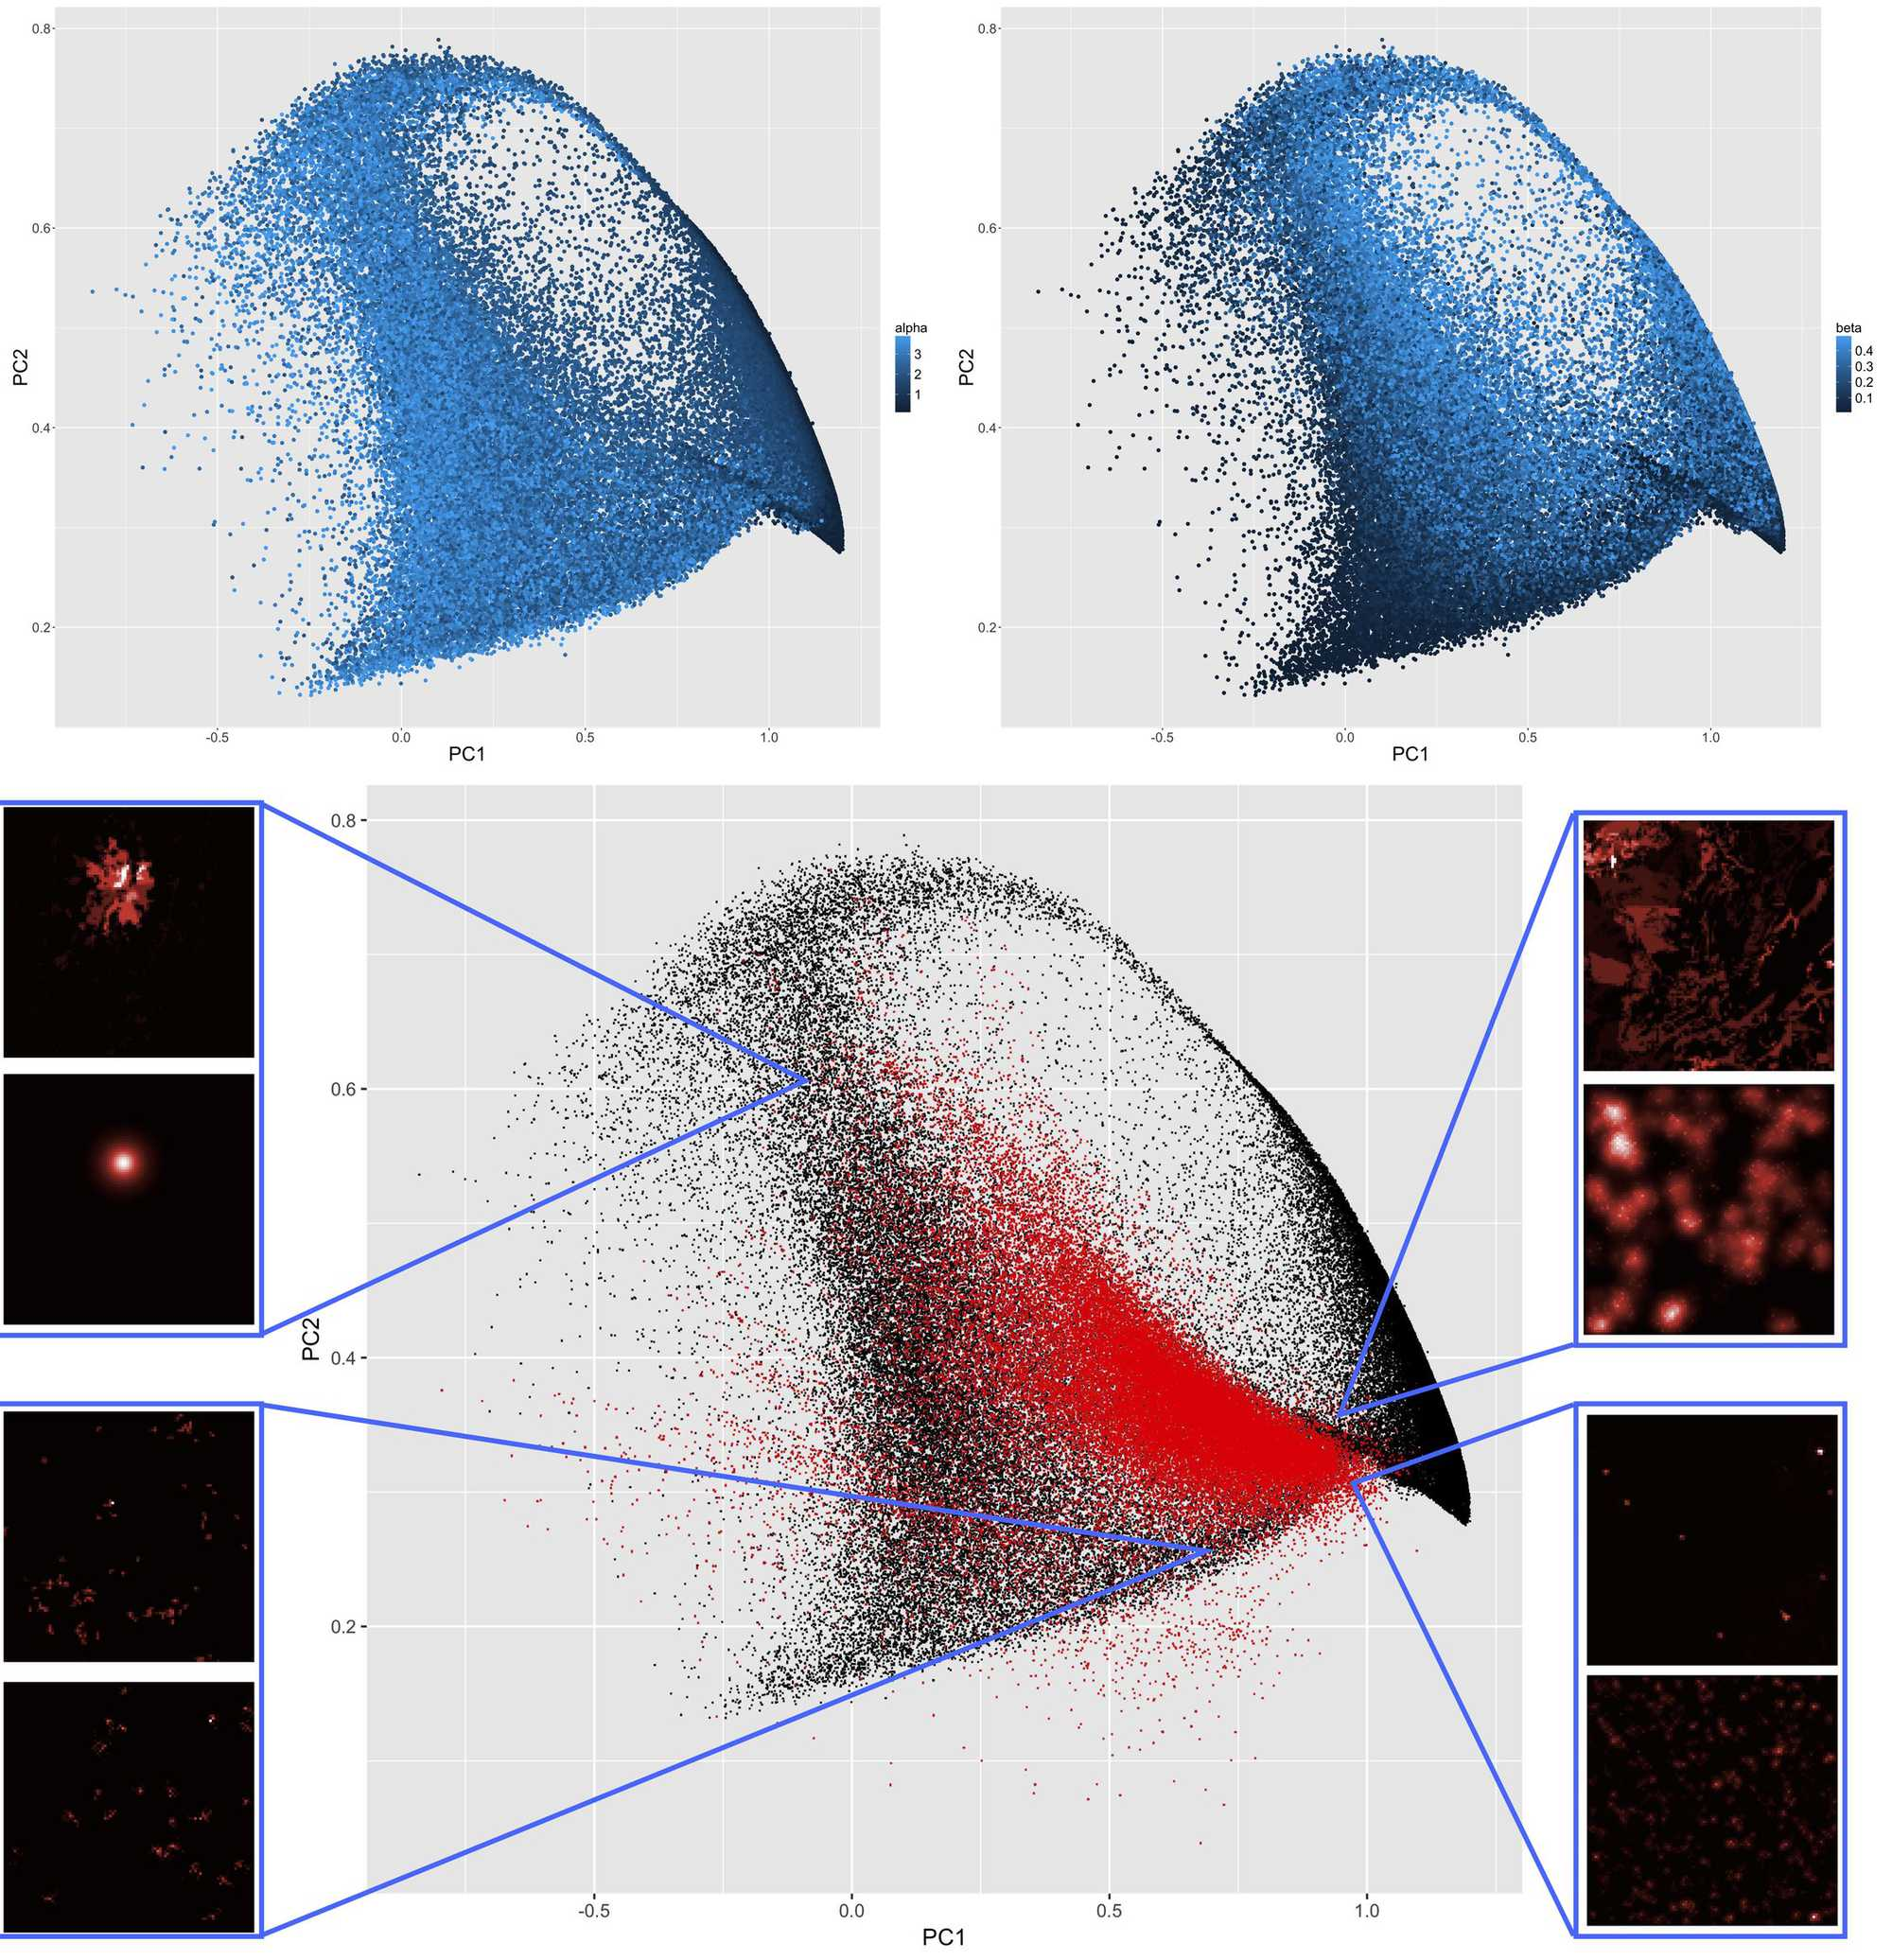
\includegraphics[width=\textwidth]{../../Figures/Final/5-2-2-fig-density-fig5.jpg}
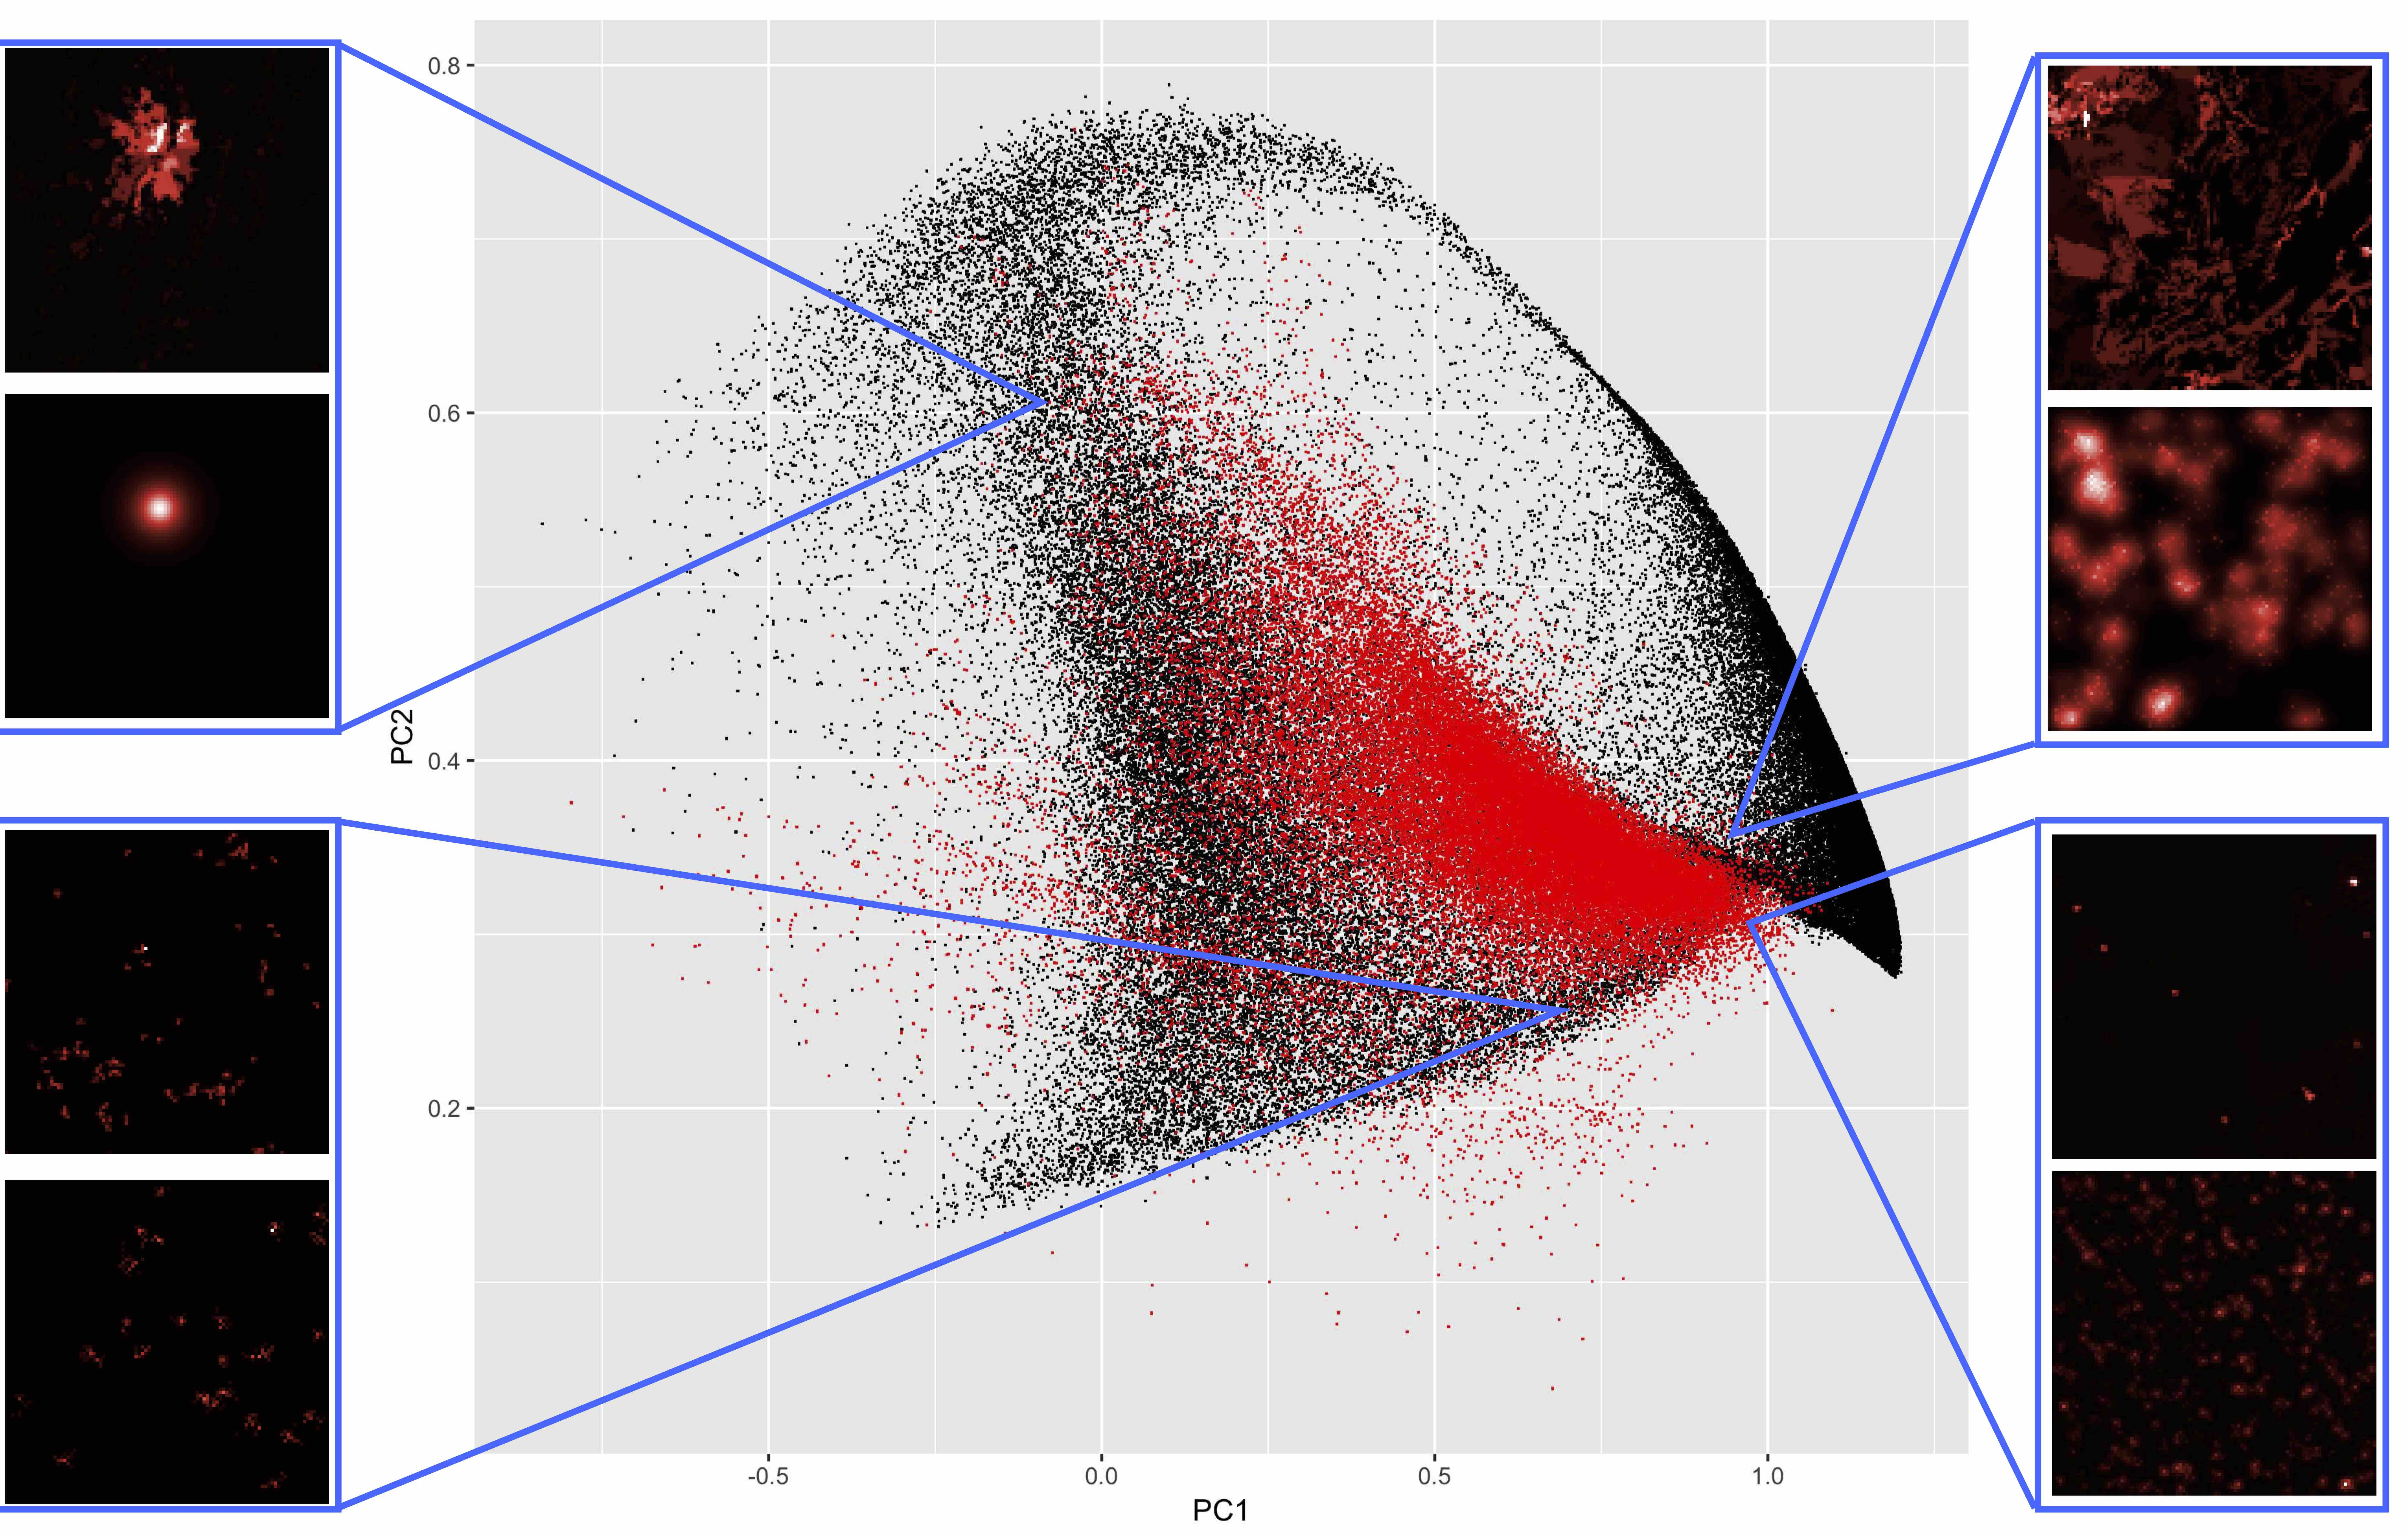
\includegraphics[width=\textwidth]{figuresraw/density_synth.jpg}


\footnotesize\textit{Brute force calibration by exploring the parameter space. Reproduction of most existing configuration in the morphological sense (here in principal plan).}

}





\sframe{Model Targeted Exploration}{

\centering

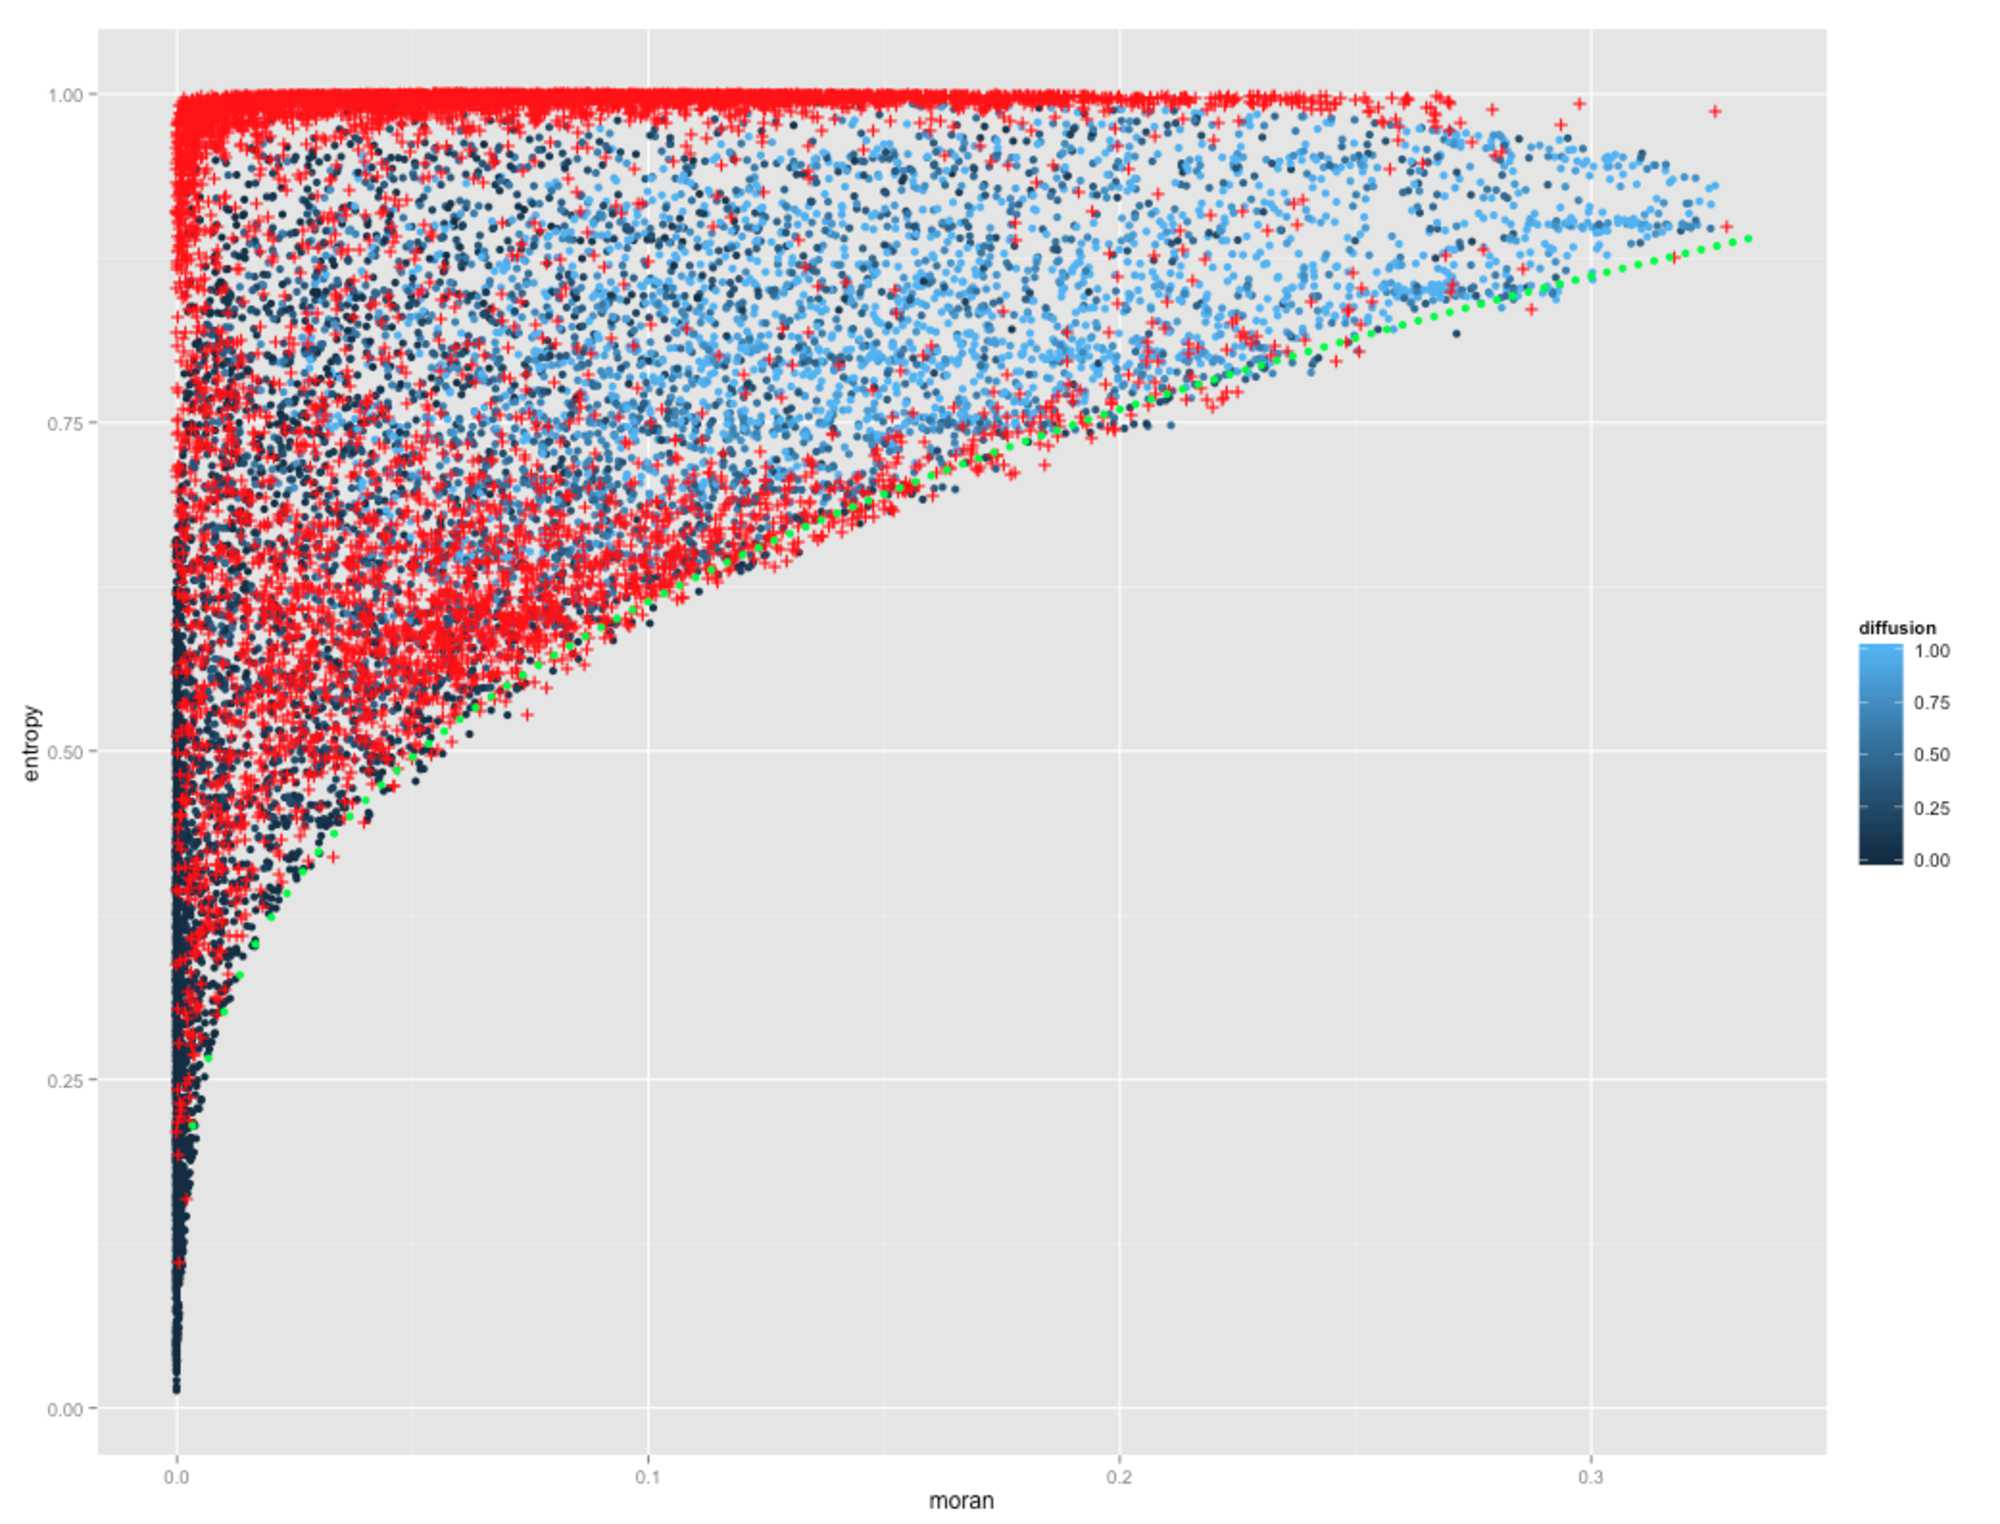
\includegraphics[width=0.8\textwidth]{../../Figures/Final/5-2-2-fig-density-fig6.jpg}

\footnotesize\textit{Potentialities of targeted model explorations: here feasible space using Pattern Space Exploration algorithm \cite{10.1371/journal.pone.0138212}.}

}





\sframe{Model classification : PDE}{

%% derived PDE

The one-dimensional model verifies the PDE :

\begin{equation}\label{eq:pde}
\begin{split}
\delta t \cdot \frac{\partial p}{\partial t} = \frac{N_G \cdot p^{\alpha}}{P_{\alpha}(t)} + \frac{\alpha \beta (\alpha - 1) \delta x^2}{2}\cdot \frac{N_G \cdot p^{\alpha-2}}{P_{\alpha}(t)} \cdot \left(\frac{\partial p}{\partial x}\right)^2\\
+ \frac{\beta \delta x^2}{2} \cdot \frac{\partial^2 p}{\partial x^2} \cdot\left[ 1 + \alpha \frac{N_G p^{\alpha - 1}}{P_{\alpha(t)}} \right]
\end{split}
\end{equation}

}


\sframe{Stationary behavior of 1D model}{

\centering
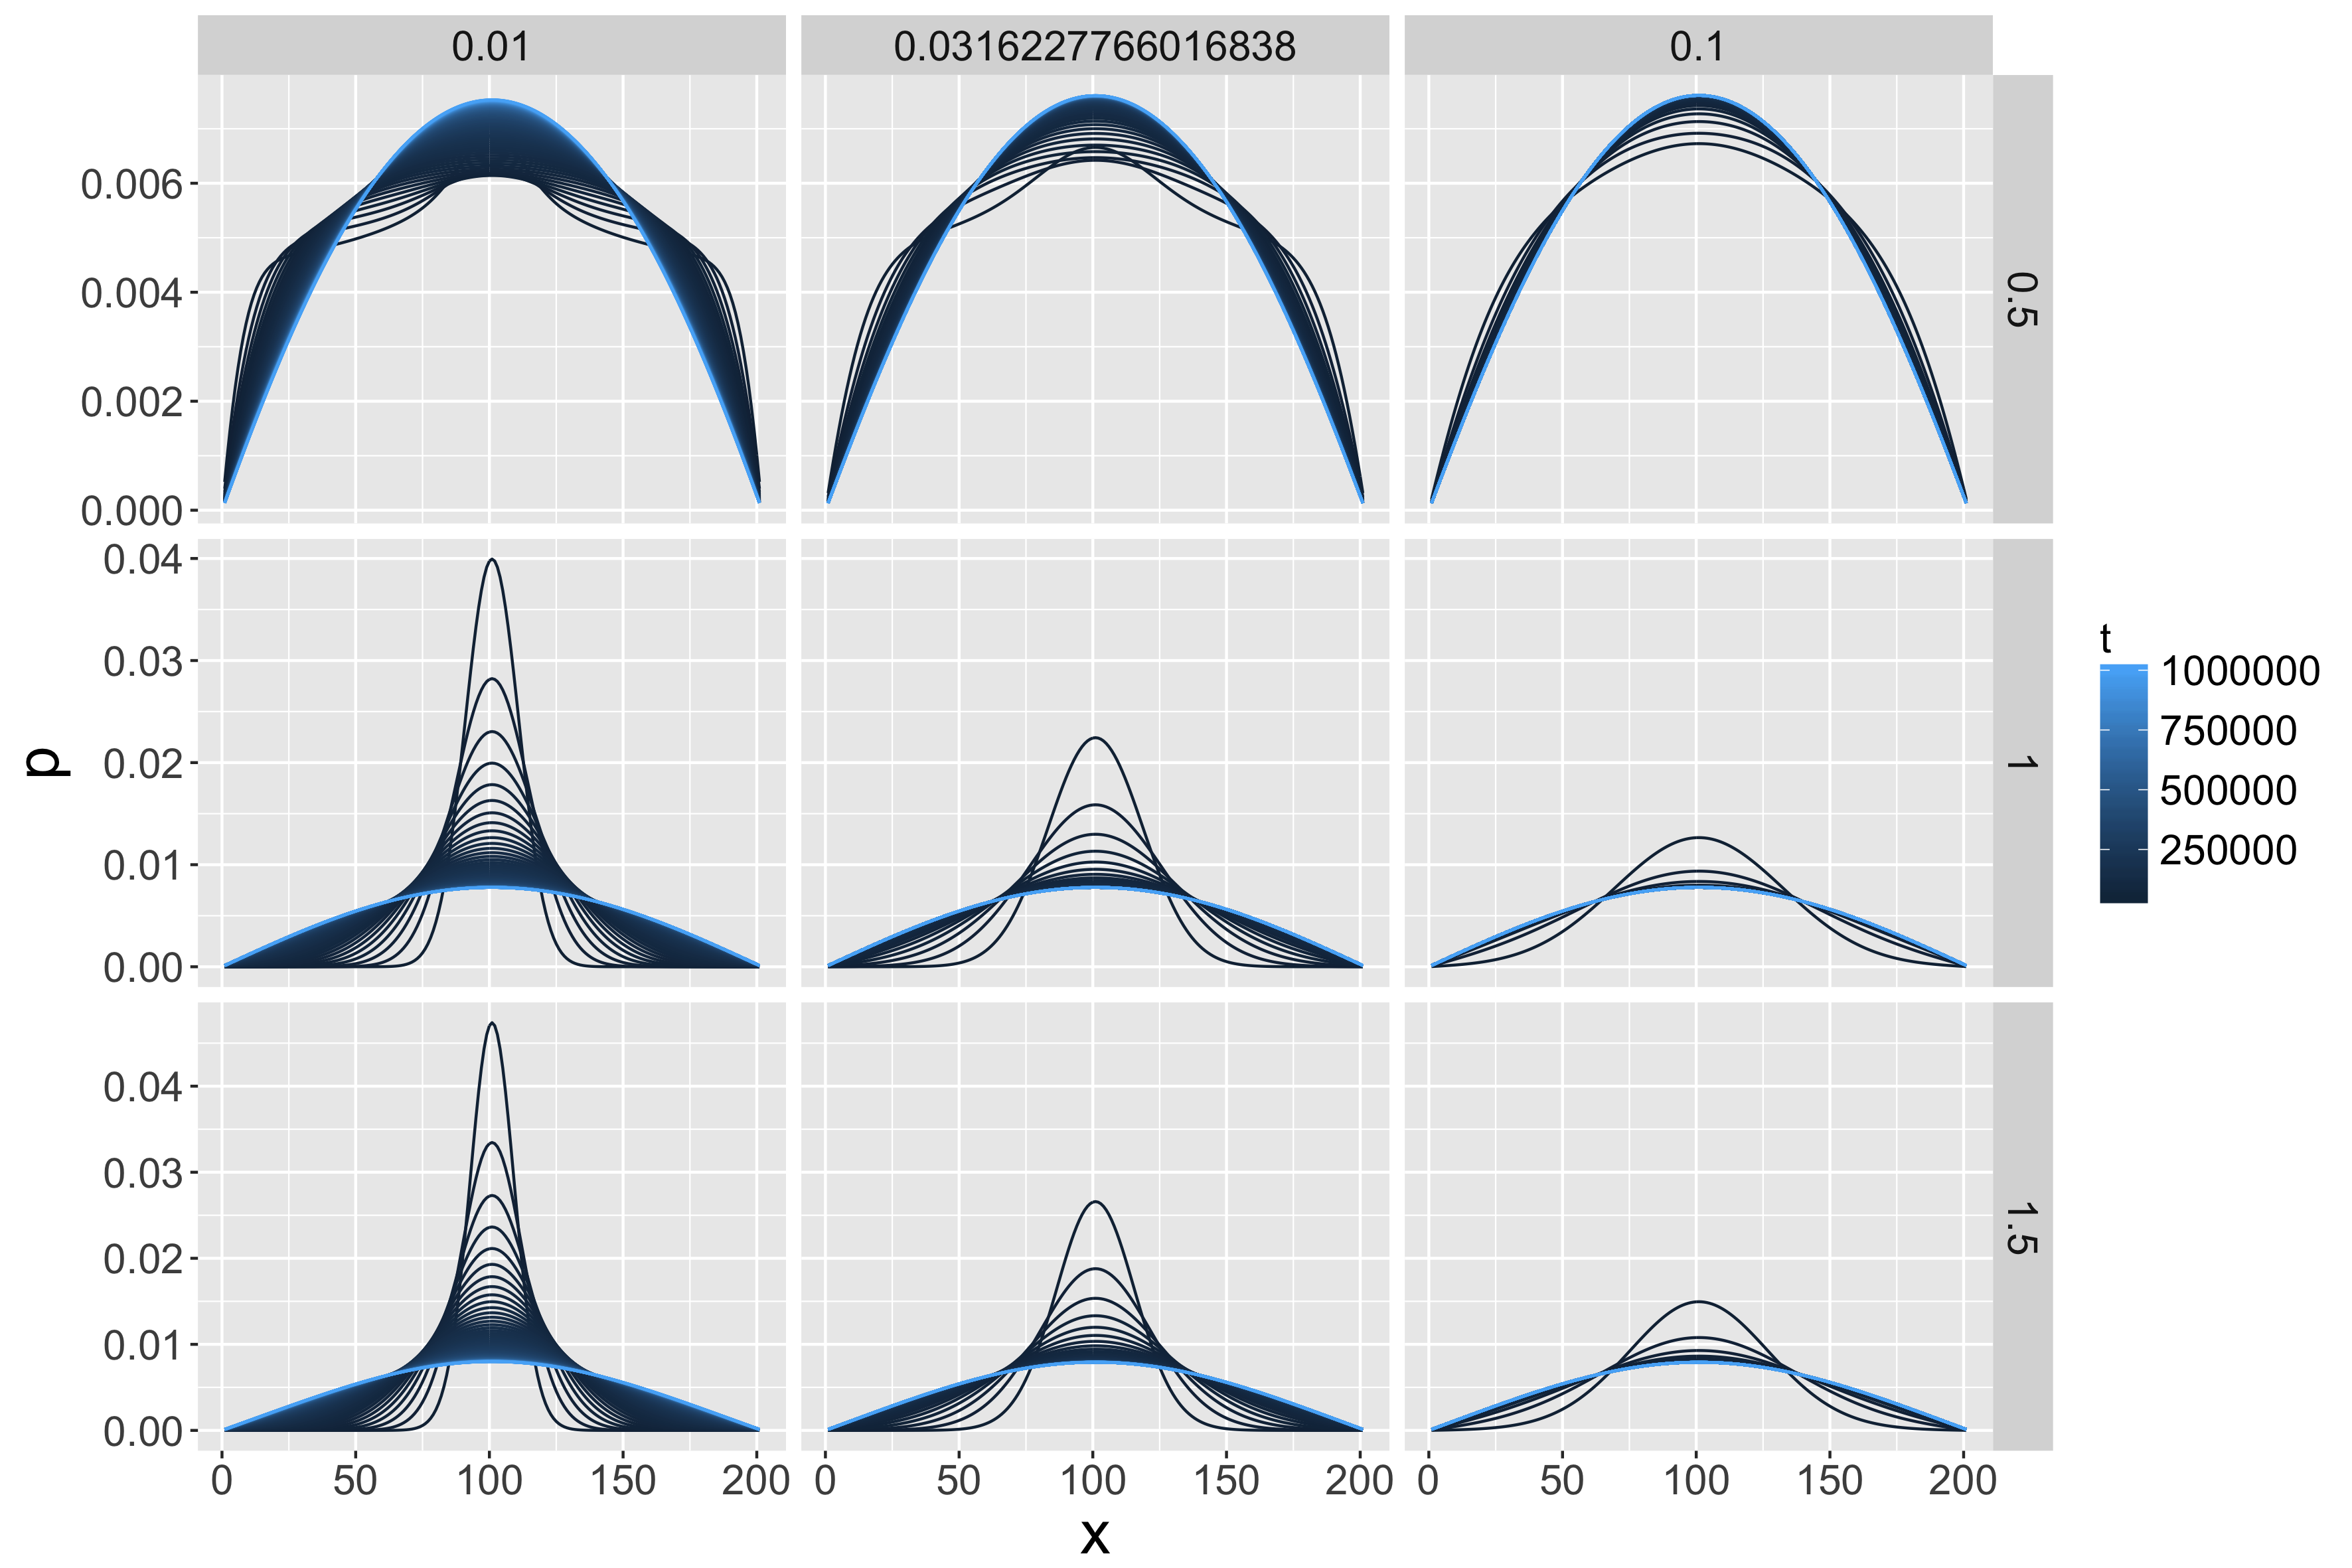
\includegraphics[width=\textwidth]{figuresraw/density_stationary}
}

\sframe{Stationary behavior of 1D model}{
\centering
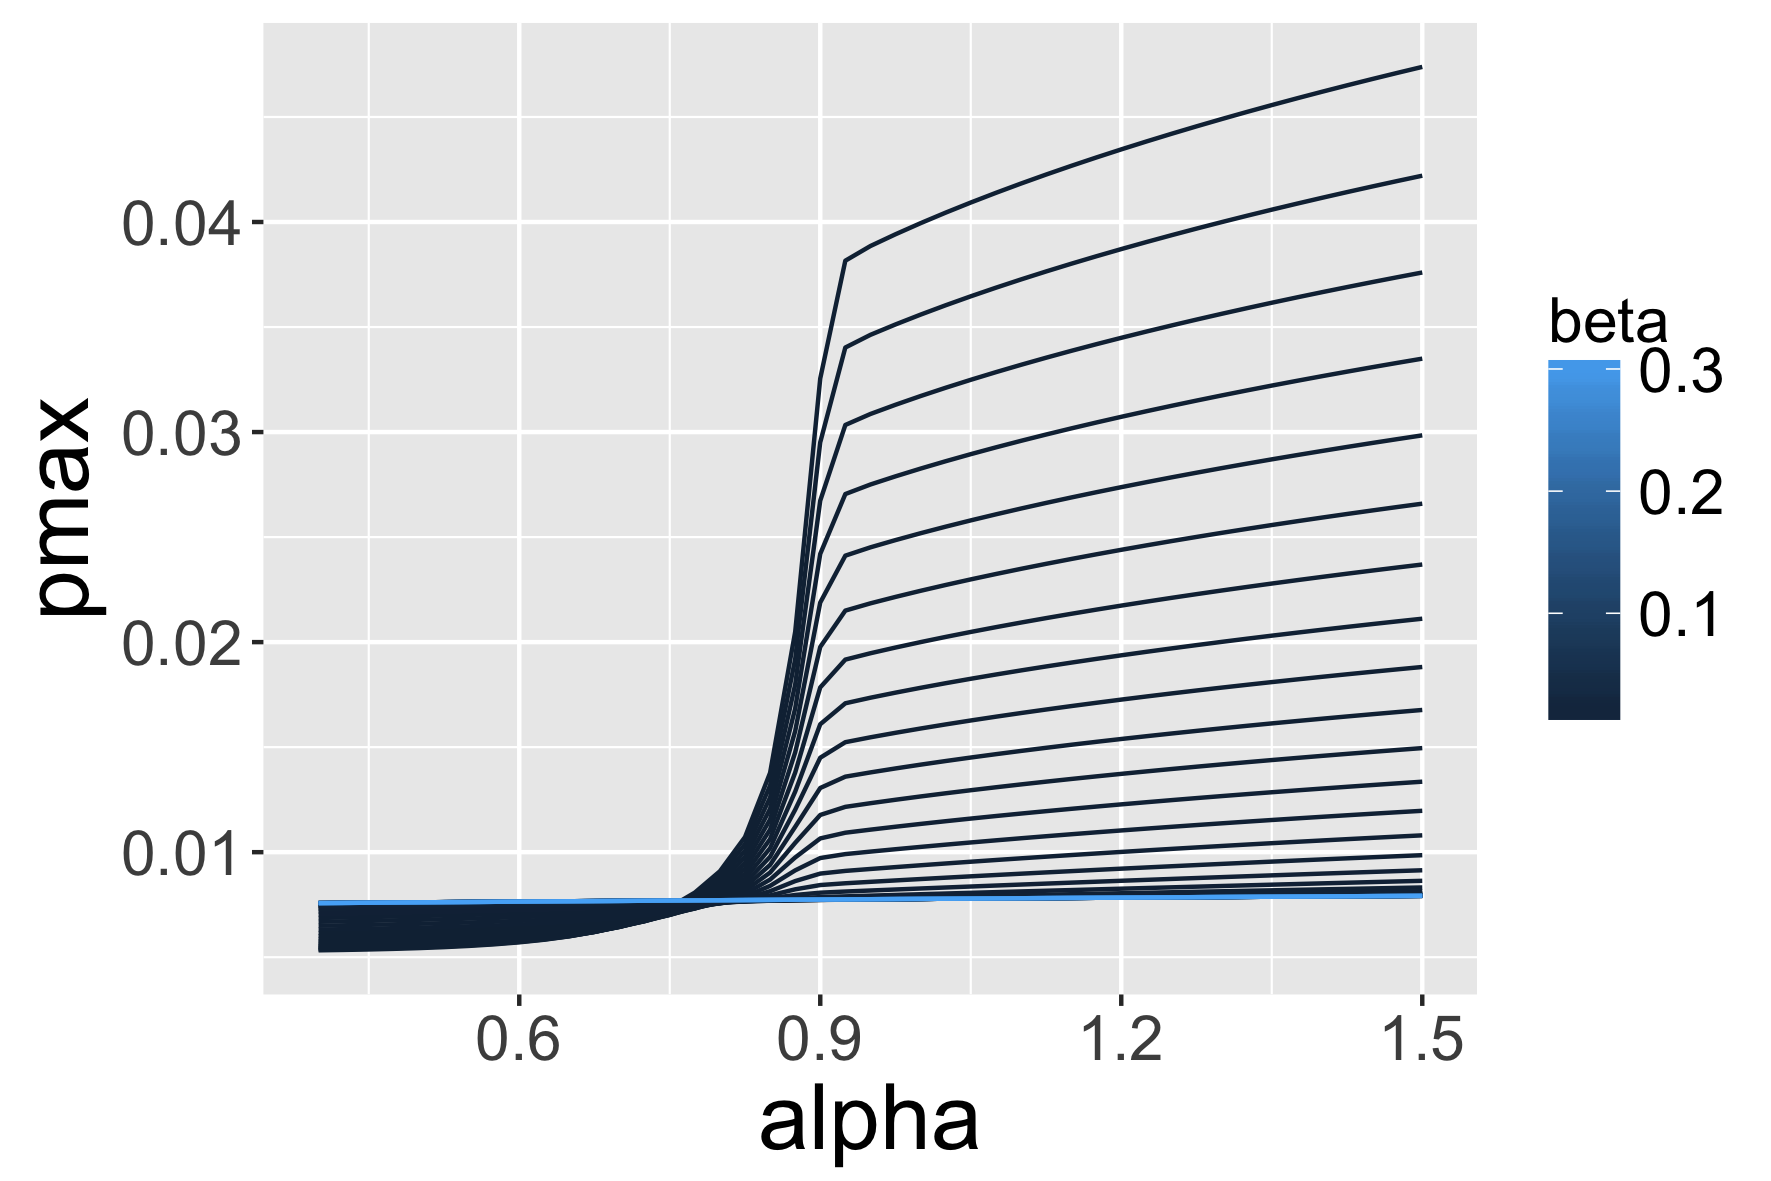
\includegraphics[width=0.48\textwidth]{figuresraw/density_pmax_alpha}
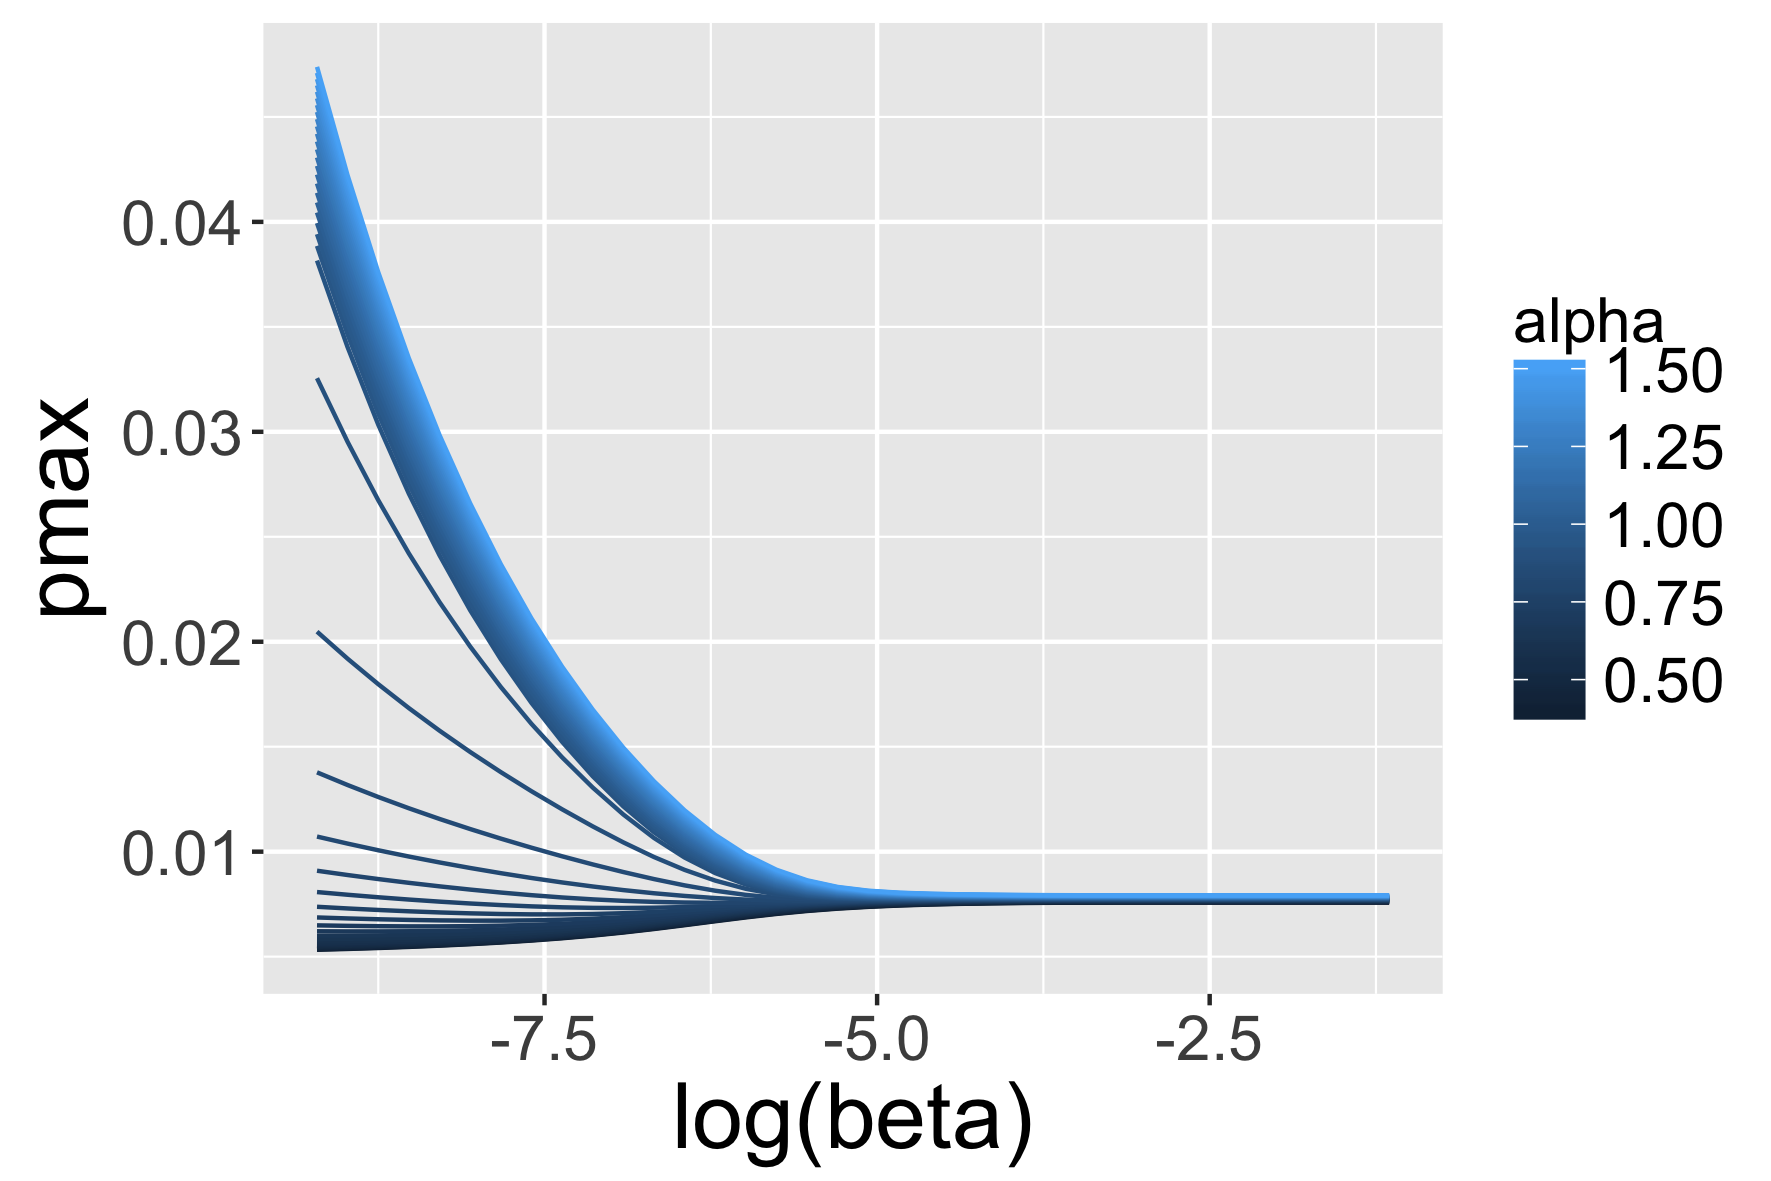
\includegraphics[width=0.48\textwidth]{figuresraw/density_pmax_logbeta}

}



\sframe{Morphological indicators}{

\begin{enumerate}
\item Rank-size slope $\gamma$, given by $\ln \left( P_{\tilde{i}}/P_0\right) \sim k + \gamma\cdot \ln \left(\tilde{i}/i_0\right)$ where $\tilde{i}$ are the indexes of the distribution sorted in decreasing order.
\item Entropy of the distribution:
\begin{equation}
\mathcal{E} = \sum_{i=1}^{M}\frac{P_i}{P}\cdot \ln{\frac{P_i}{P}}
\end{equation}
$\mathcal{E}=0$ means that all the population is in one cell whereas $\mathcal{E}=0$ means that the population is uniformly distributed.
\item Spatial-autocorrelation given by Moran index, with simple spatial weights given by $w_{ij} = 1/d_{ij}$
\[
I = M \cdot \frac{\sum_{i\neq j} w_{ij} \left(P_i - \bar{P}\right)\cdot\left(P_j - \bar{P}\right)}{\sum_{i\neq j} w_{ij} \sum_{i}{\left( P_i - \bar{P}\right)}^2}
\]
\item Mean distance between individuals
\[
\bar{d} = \frac{1}{d_M}\cdot \sum_{i<j} \frac{P_i P_j}{P^2} \cdot d_{ij}
\]
where $d_M$ is a normalisation constant
\end{enumerate}



}


\sframe{Model behavior : Convergence}{

Large number of repetitions show good convergence properties

%% hist examples

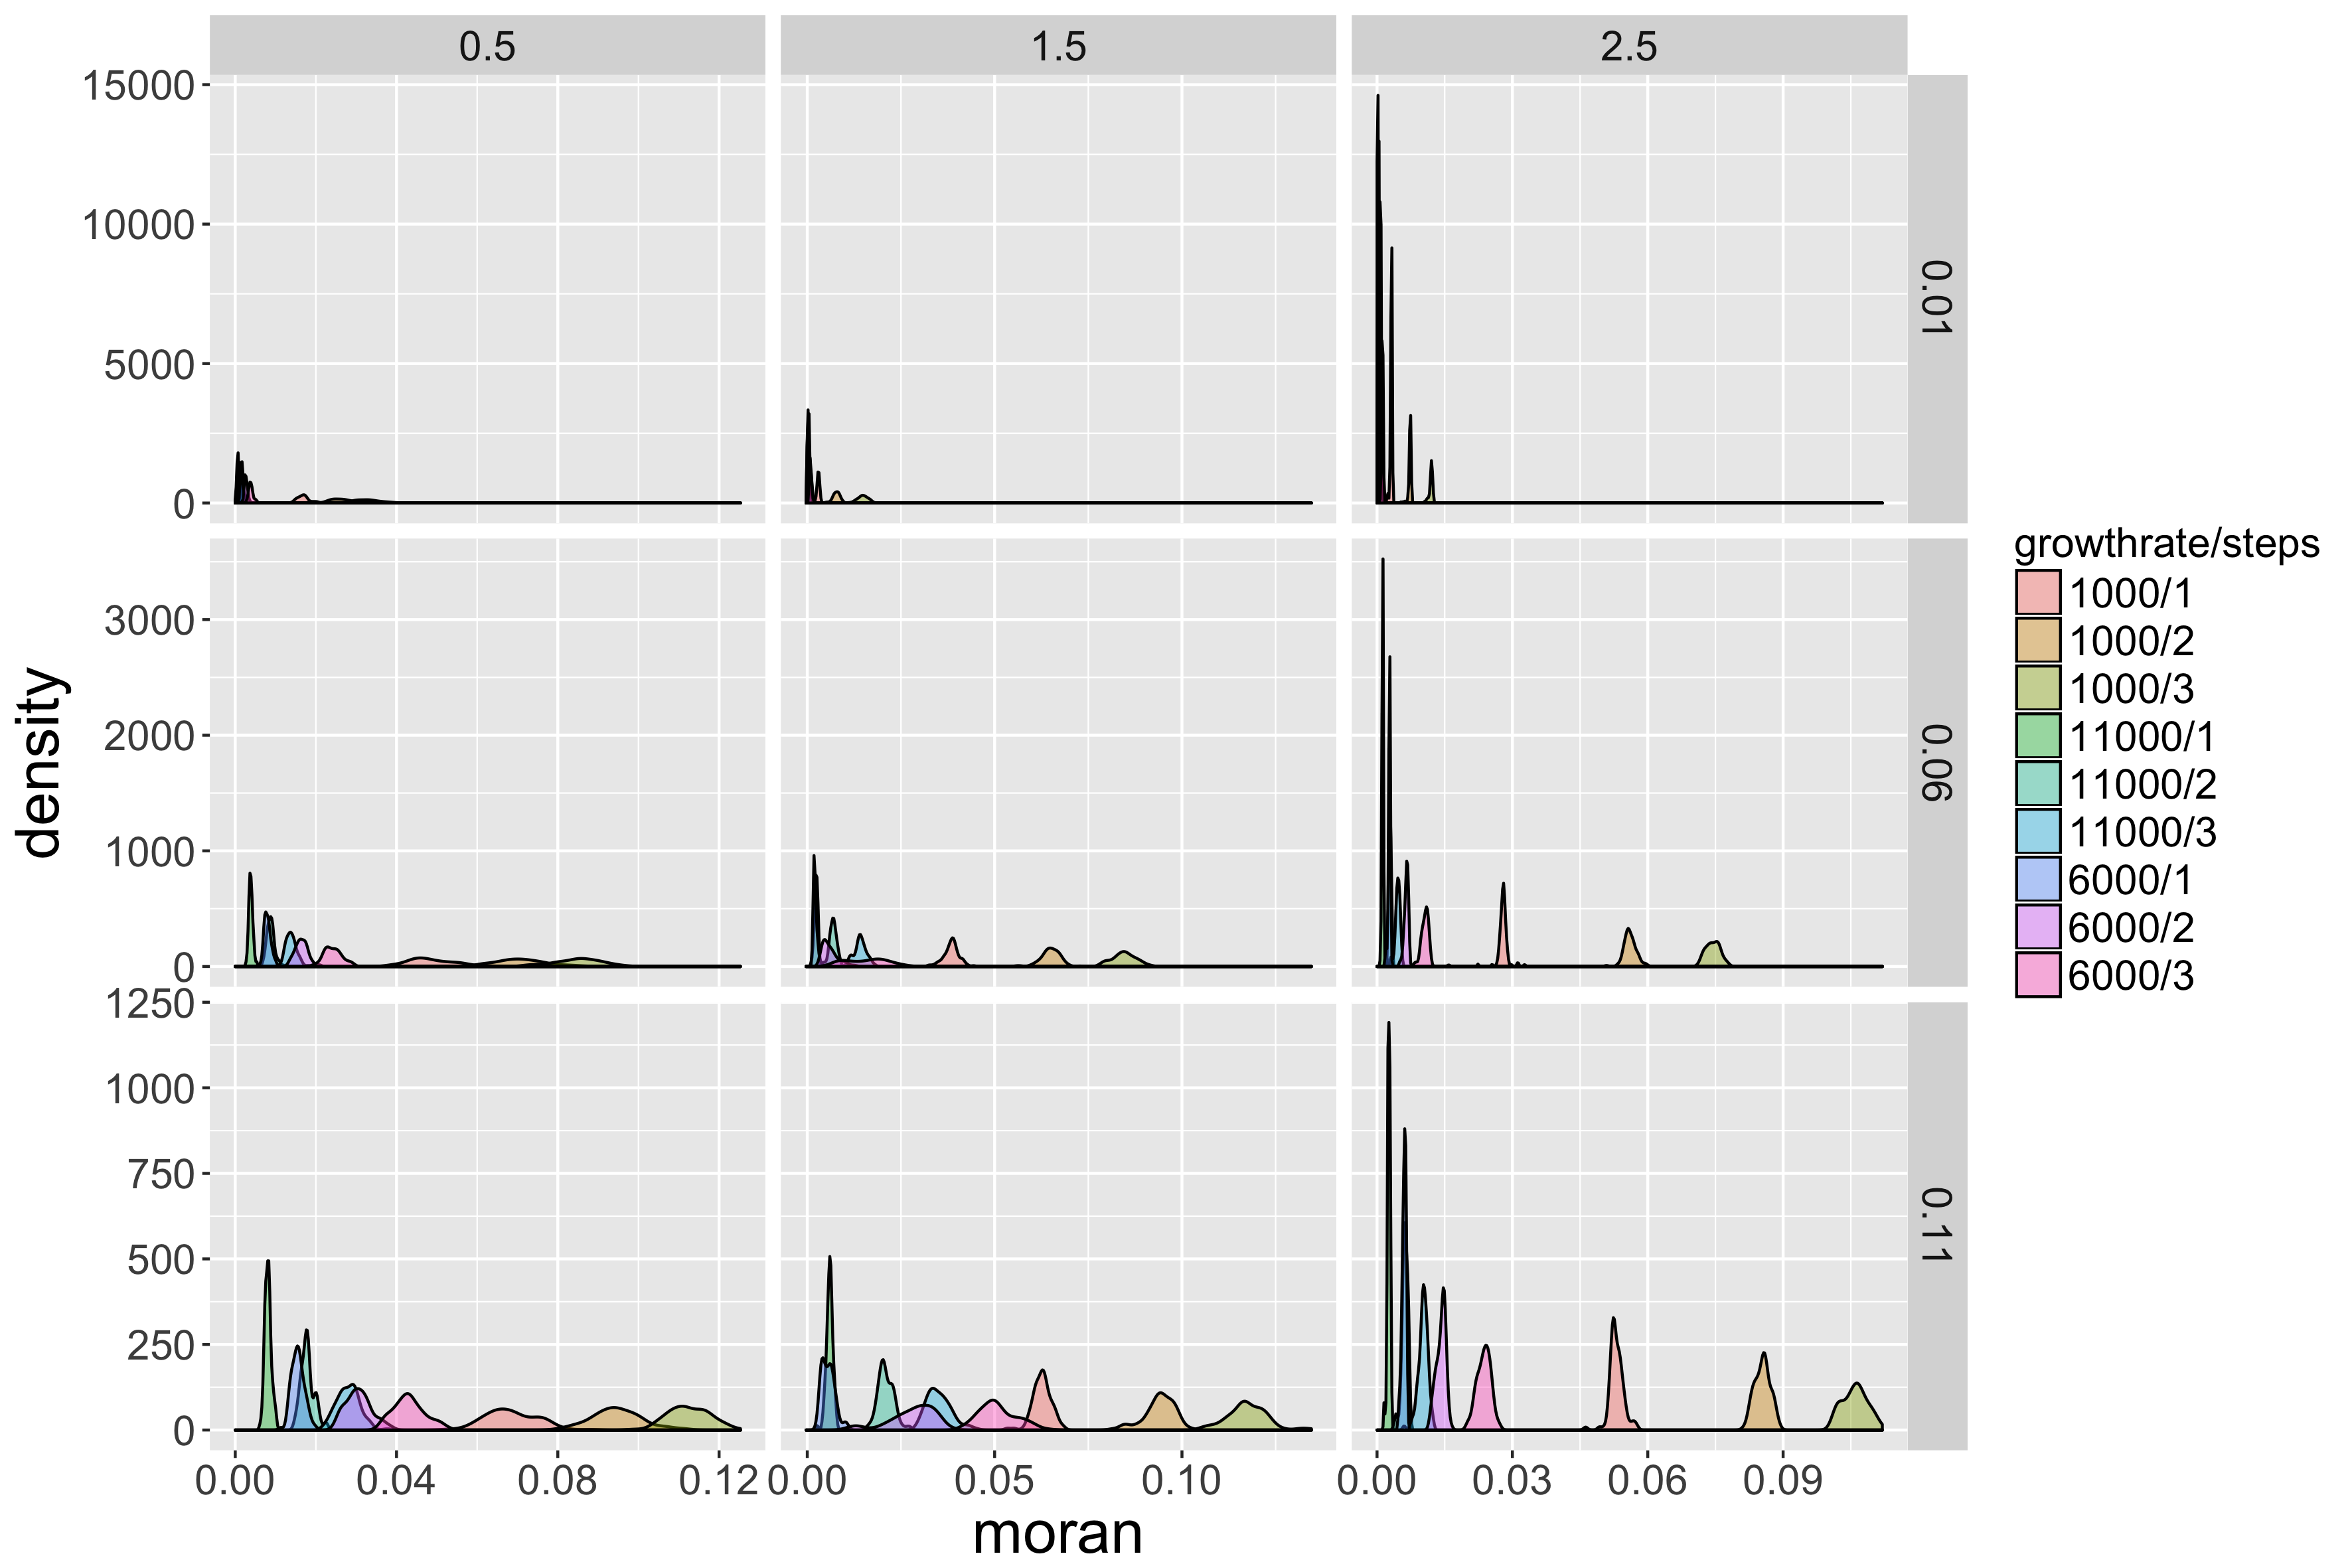
\includegraphics[width=0.5\textwidth]{figuresraw/density_hist_moran}
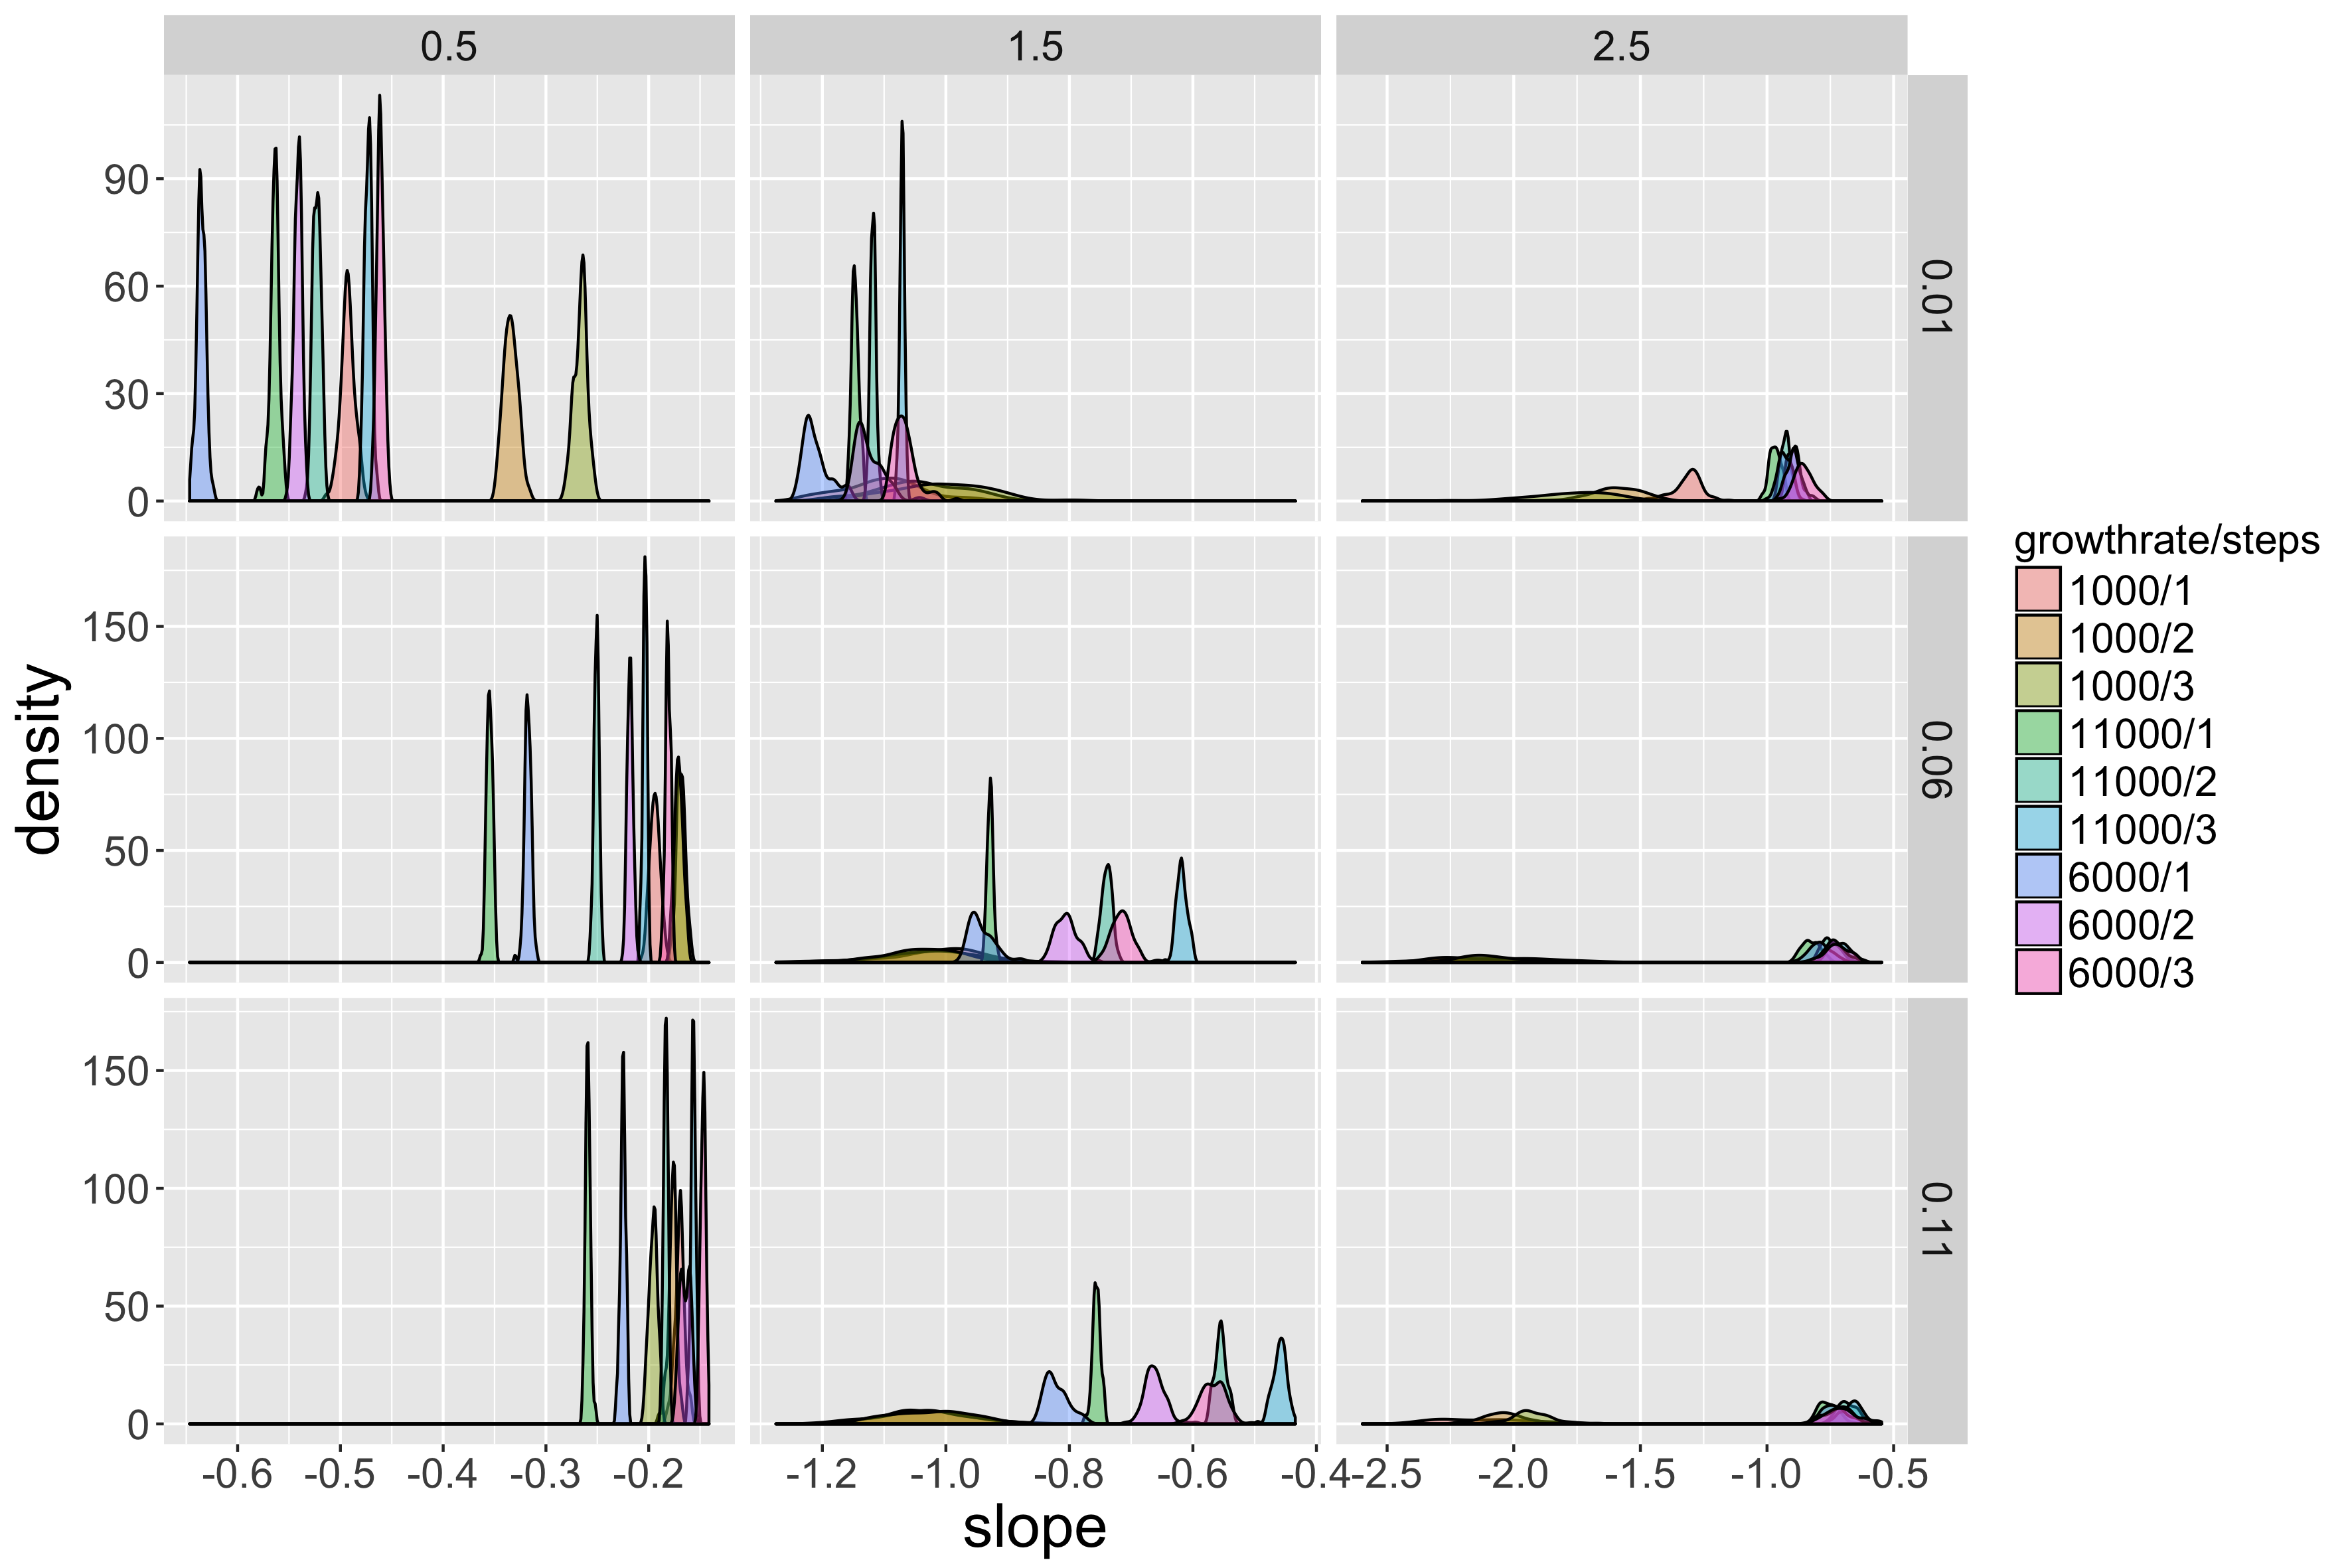
\includegraphics[width=0.5\textwidth]{figuresraw/density_hist_slope}

}


\sframe{Model behavior}{


\includegraphics[width=0.5\textwidth]{figuresraw/density_pc_colalpha}
\includegraphics[width=0.5\textwidth]{figuresraw/density_pc_colbeta}

}


\sframe{Empirical indicators computation}{

$\rightarrow$ Eurostat population density raster (100m, simplified at 500m resolution)

\medskip

$\rightarrow$ Overlapping (10km offset) squares of 50km side : equivalent to smoothing, removes window shape effect. Not very sensitive to window size (tested with 30km and 100km)

\medskip

$\rightarrow$ Indicators computed using Fast Fourier Transform Convolution

\medskip

$\rightarrow$ Classification using repeated k-means ; number of clusters taken at transition in clustering coefficient.

}

\sframe{Model calibration: all indicators}{

\centering
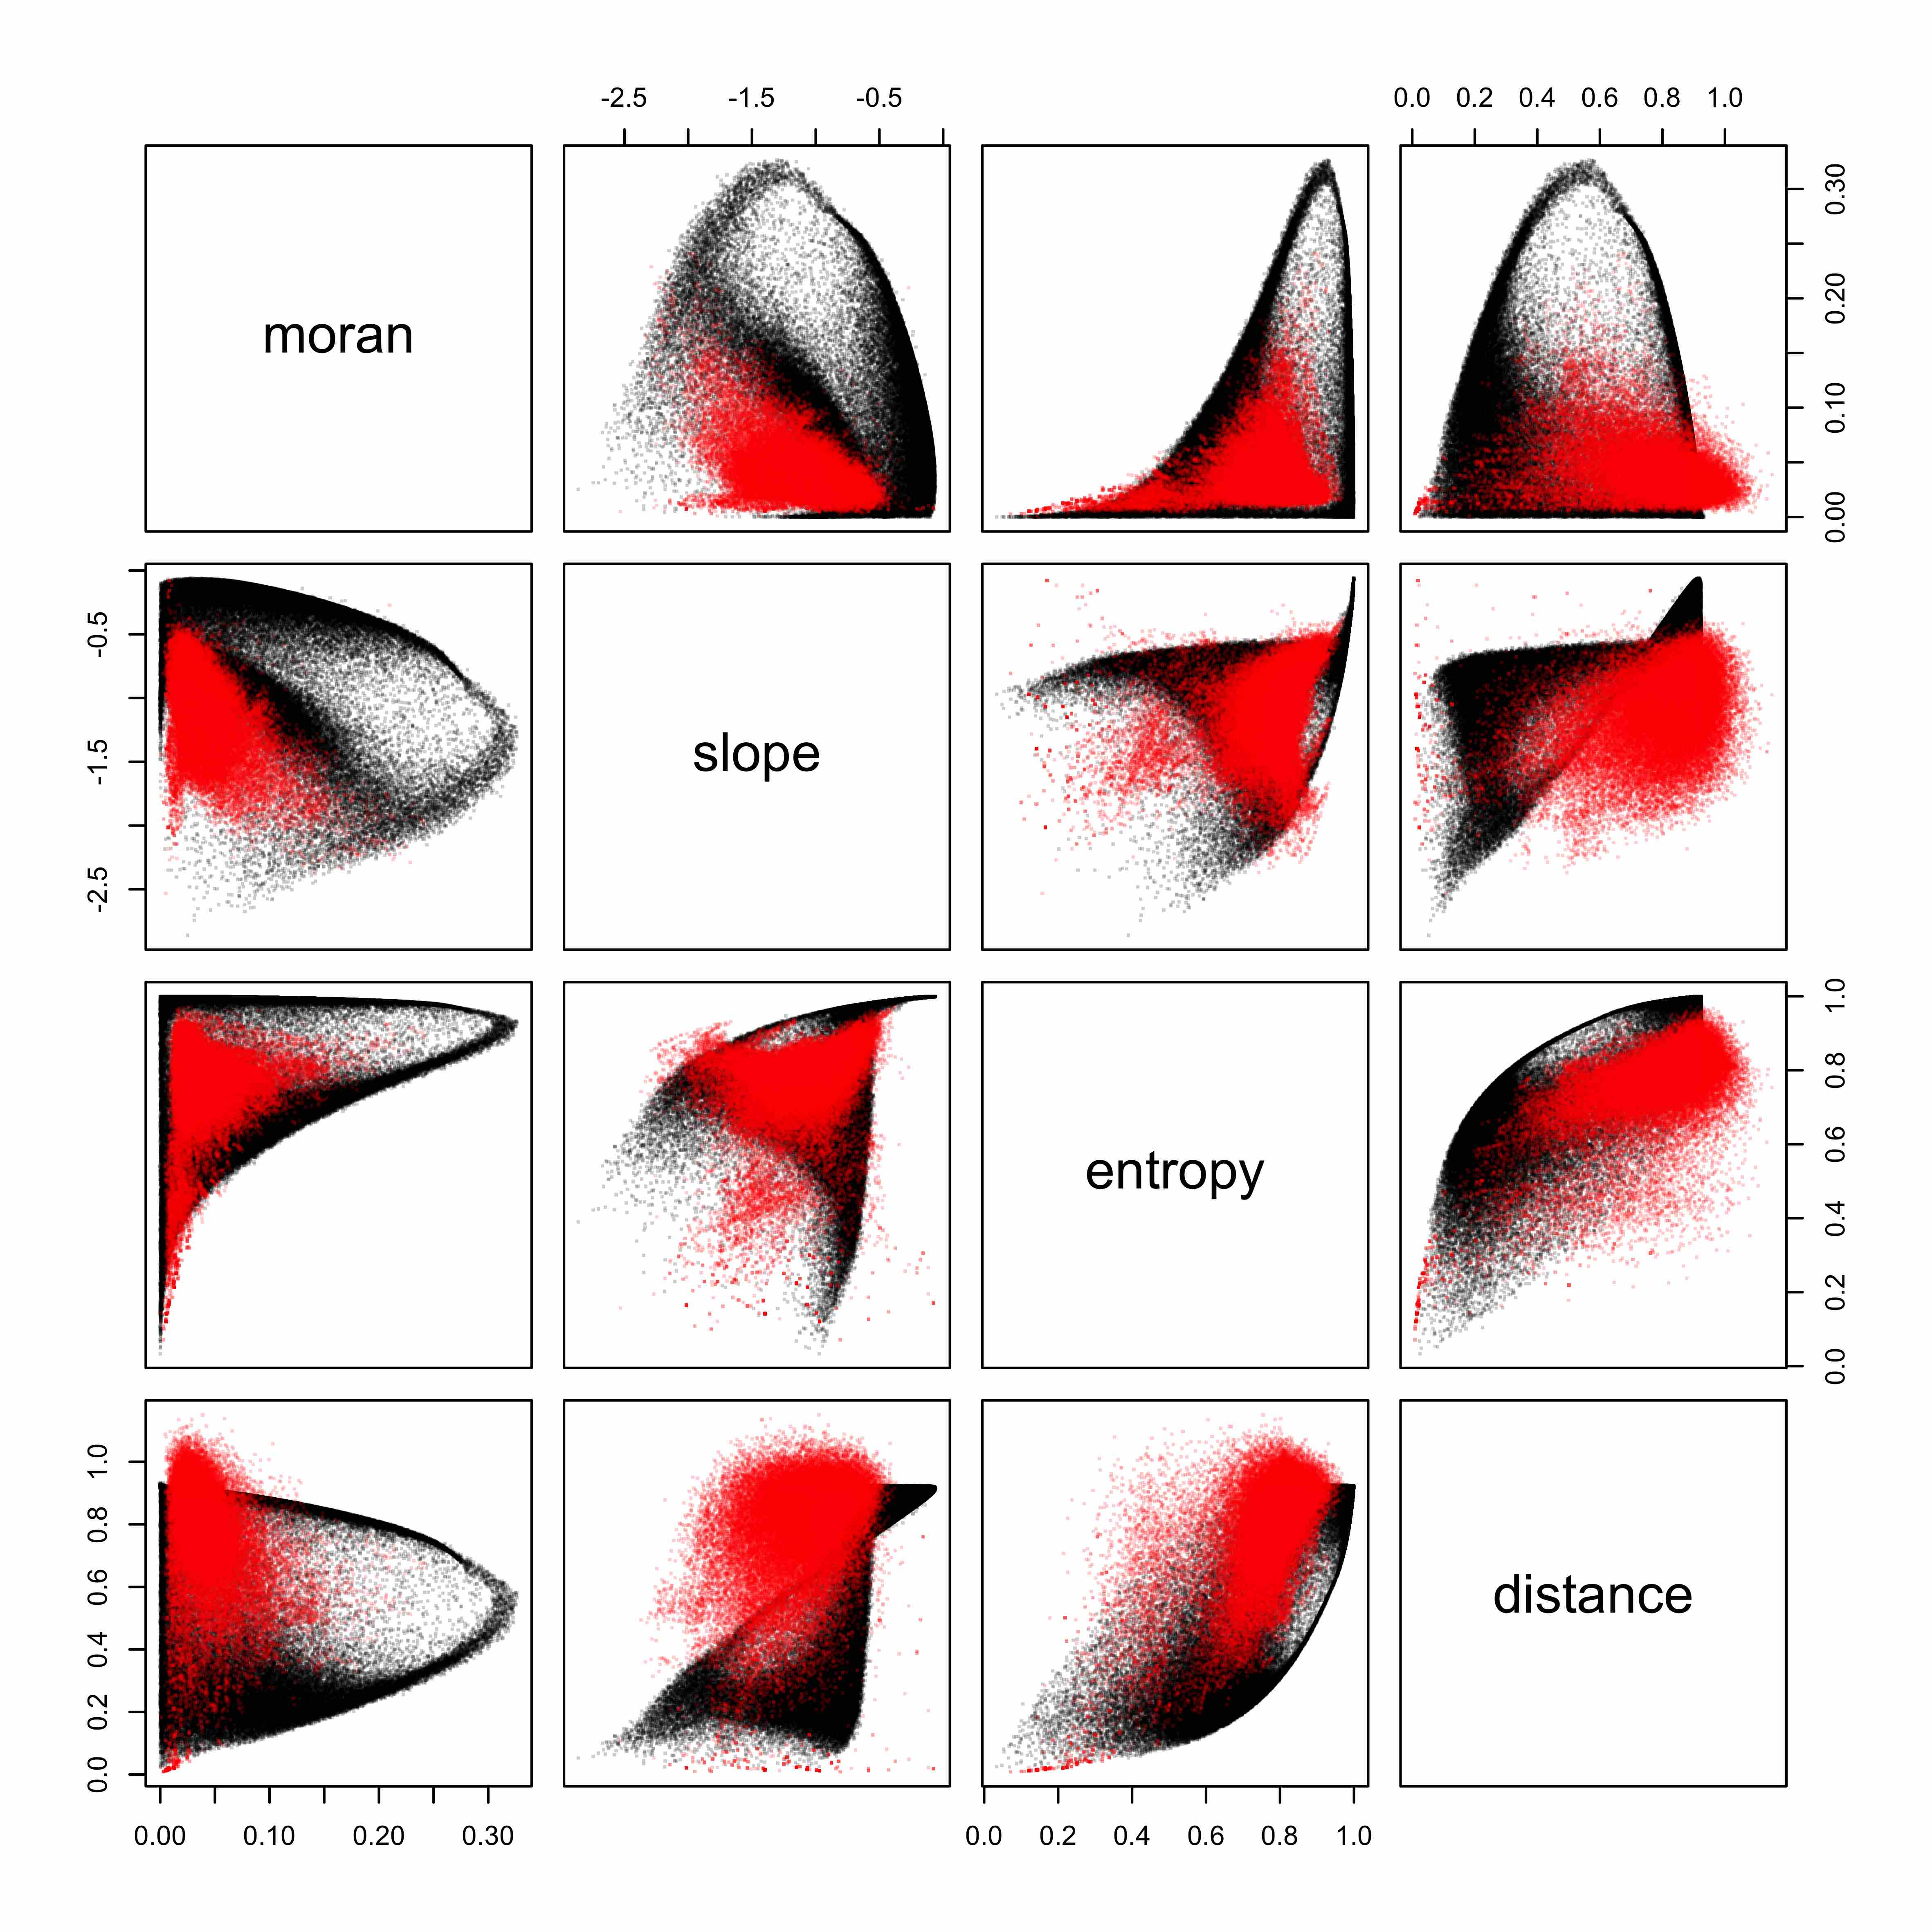
\includegraphics[width=0.8\textwidth]{figuresraw/density_scatter}

}







%\section*{Mesoscopic co-evolution}
% TODO Mesoscopic co-evolution



\sframe{Including more complex processes ?}{

%
%% transition : representation of territories
%

\textit{Which ontology to include more complex functional properties ?}

\medskip

$\rightarrow$ Territorial systems as the strong coupling between territories and (potential and realized) networks \cite{dupuy1987vers}.

\medskip

$\rightarrow$ Networks convey functional notions of centralities and accessibility, among others ; have furthermore proper topological properties.


}


%



\sframe{Interactions between Networks and Territories}{

%% qualitative slide
%% eventually layus on literature with the cit nw ? maybe too much
%% def. covevol : besoin coevol regimes, annexe
%% idem macrocoevol en annexe
%
%


\textit{Complex co-evolutive processes between Territories and Transportation Networks}

\medskip

\centering

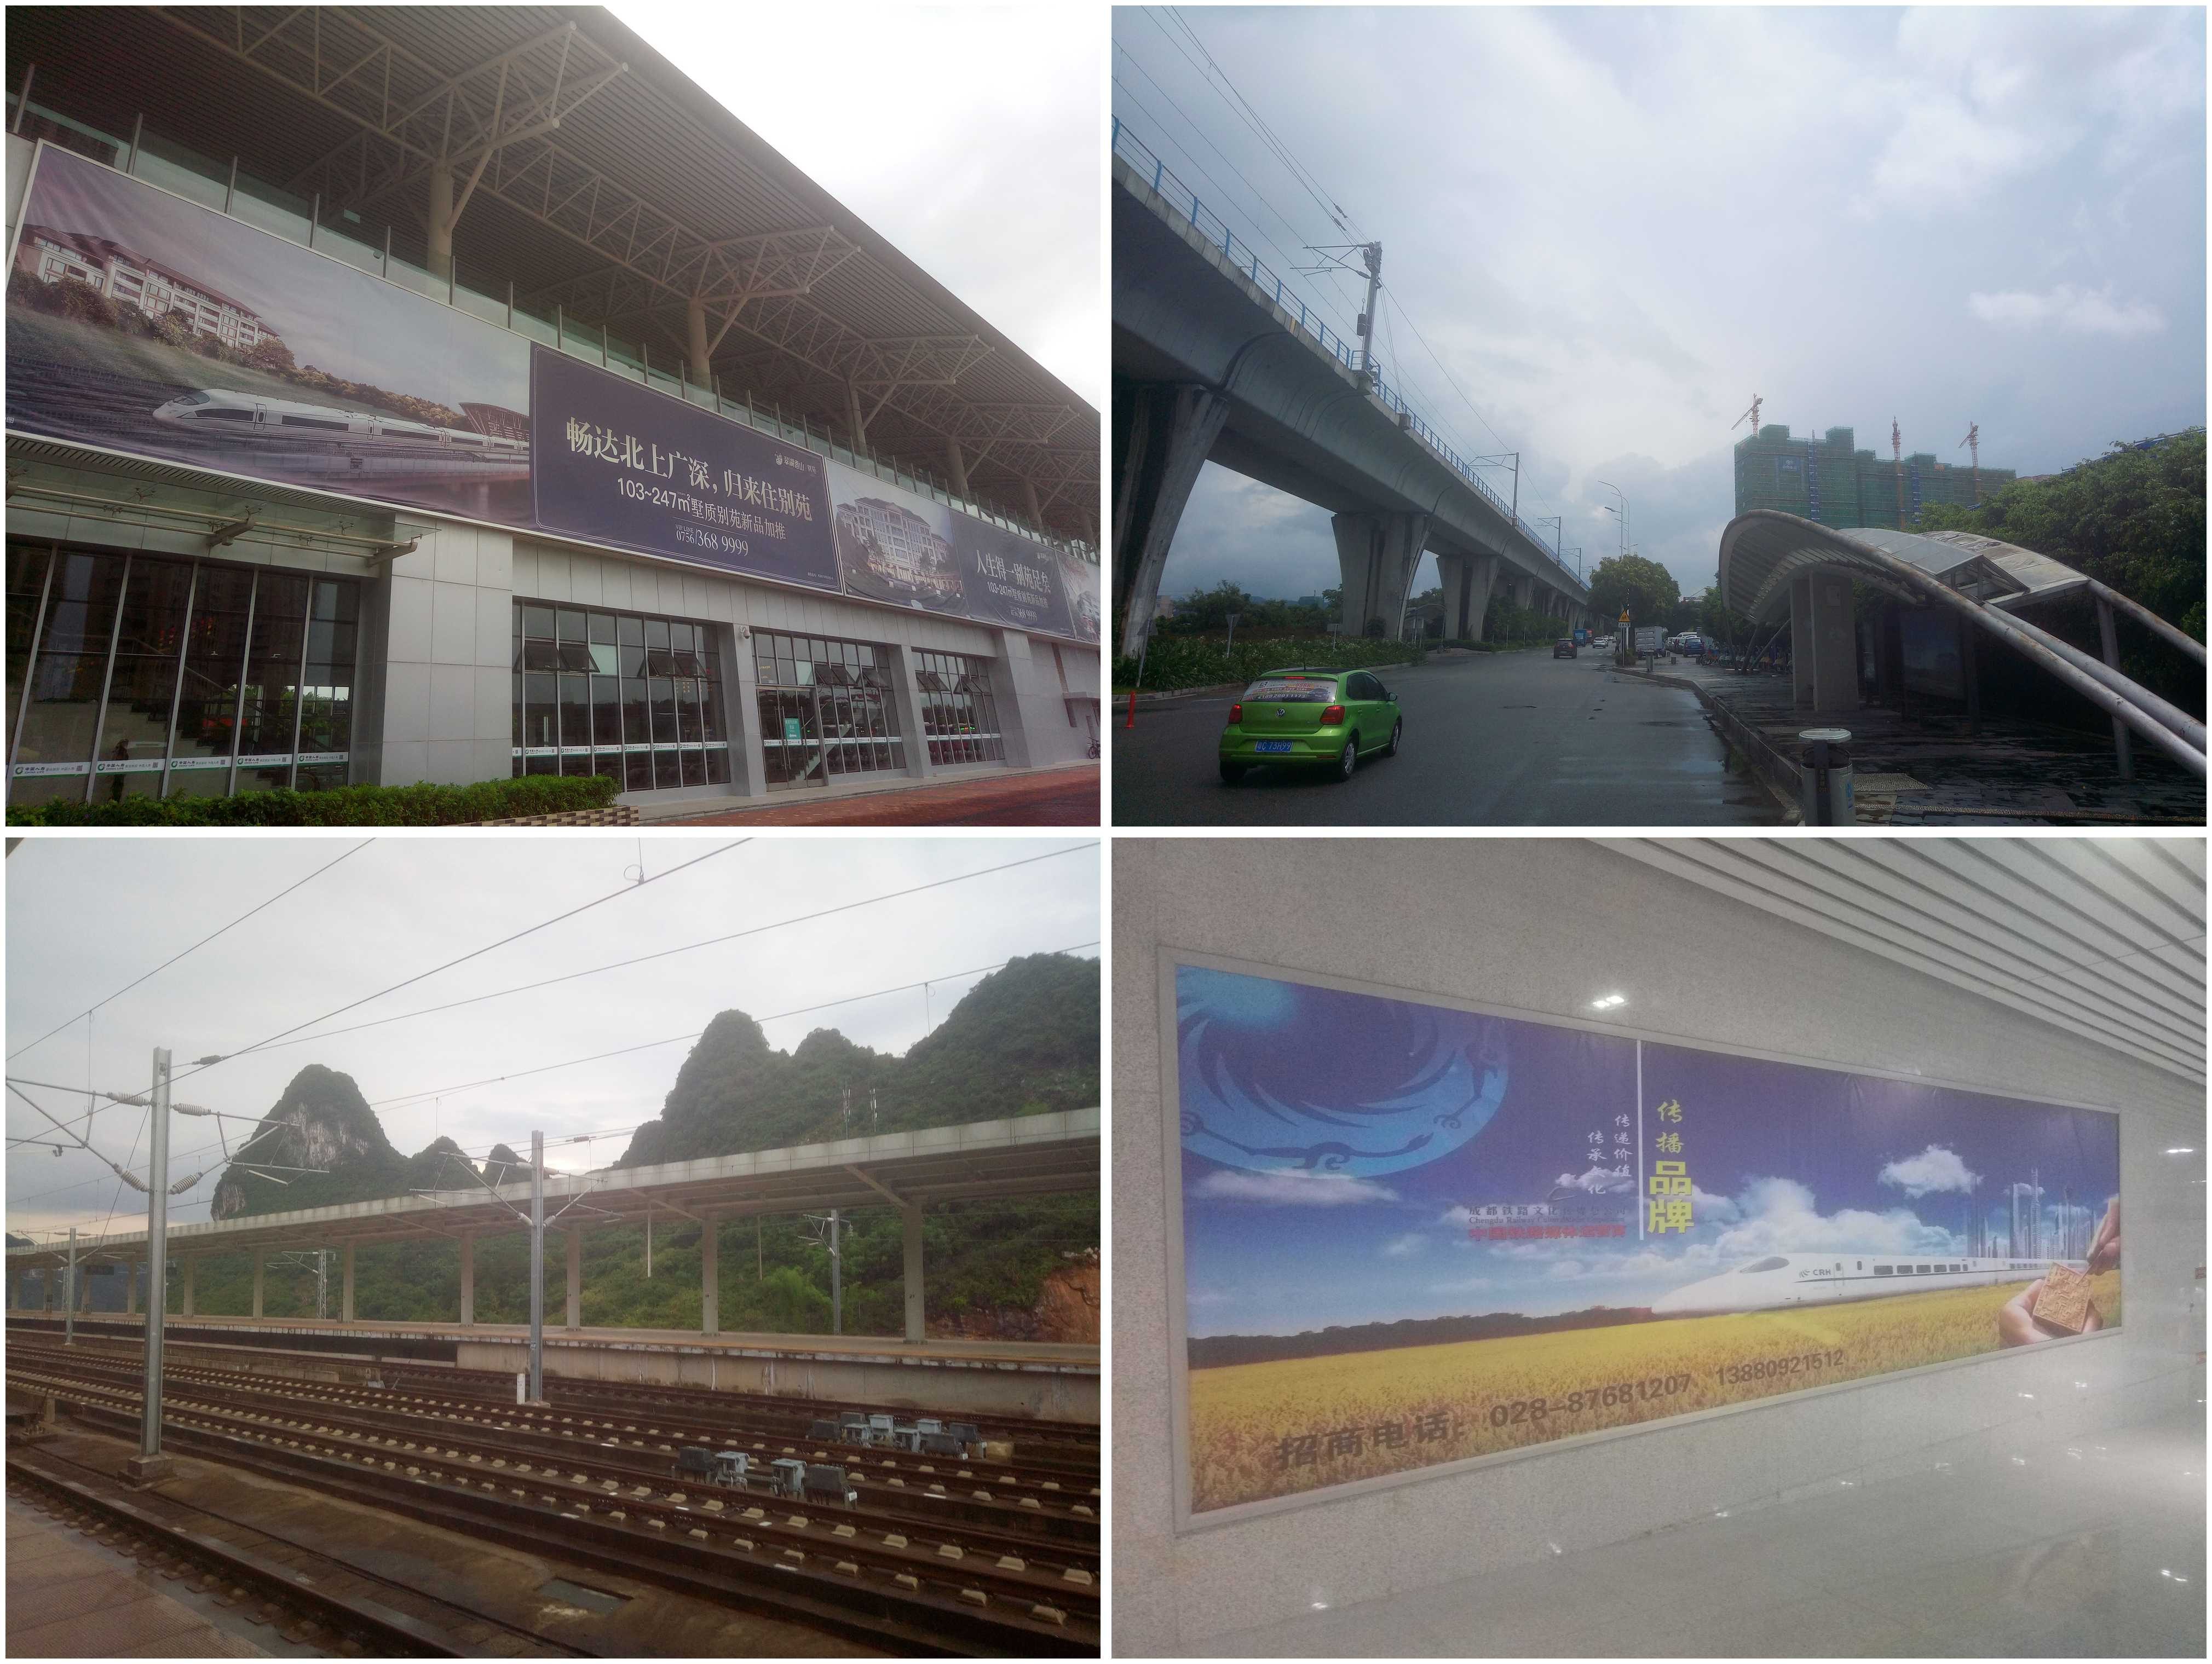
\includegraphics[height=0.7\textheight]{../../Figures/Final/1-3-1-fig-qualitative-hsr.jpg}

\footnotesize

\textit{Expanding HSR network in China and ambiguous effects (Source : fieldwork survey)}


}




\sframe{Implementations of TOD}{

\centering
\includegraphics[width=\textwidth]{../../Figures/Qualitative/tod}

}

\sframe{Co-evolution Models}{

\centering
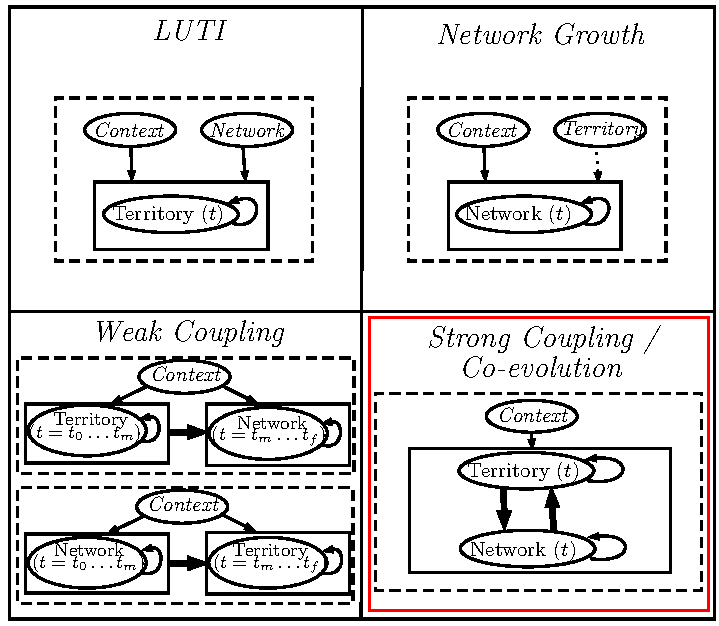
\includegraphics[width=0.8\textwidth]{figuresraw/thematic_coevolution}

}



\sframe{Defining co-evolution}{


\justify

No clear definition of co-evolution in the literature : \cite{bretagnolle:tel-00459720} distinguishes ``reciprocal adaptation'' where a sense of causality can clearly be identified, from co-evolutive regimes 


\bigskip
\bigskip

Identification of multiple causality regimes in a simple strongly coupled growth model $\rightarrow$ to be put in perspective with a theoretical definition of co-evolution based on the conjunction of Morphogenesis and the Evolutive Urban Theory, summarised by~\cite{raimbault2017co}

}



\sframe{Perspective : co-évolution}{

% def de la coevol

Proposition d'une définition de la co-évolution, basée sur une revue multi-disciplinaire :

\begin{enumerate}
	\item Existence de processus évolutifs : transformations des composantes du système territorial aux différentes échelles
	\item Trois manifestations de la co-évolution à des niveaux emboités :
	\begin{itemize}
		\item Entités en relations causales circulaires
		\item Population d'entités dans une région géographique, identifiable en pratique par les régimes de causalité
		\item Niveau global du système, interdépendance forte
	\end{itemize} 
	\item Existence de sous-systèmes en relative isolation spatio-temporelle où s'opèrent différentes co-évolutions (lien avec le concept de morphogenèse
\end{enumerate}




}




\sframe{Modeling Co-evolution}{

\justify

\cite{baptistemodeling} system dynamics with evolving capacities
 
\cite{wu2017city} population diffusion and network growth

\cite{blumenfeld2010network} and \cite{schmitt2014modelisation} : random potential breakdown for network growth.

\cite{barthelemy2009co} geometrical network growth model making network topology co-evolve with vertex density

}





%
%
%


\sframe{A Morphogenesis Model of co-evolution}{

\justify

\vspace{-1cm}

$\rightarrow$ Coupled grid population distribution and vector transportation network, following the core of \cite{raimbault2014hybrid}

\medskip

$\rightarrow$ Local morphological and functional variables determine a patch-value, driving new population attribution through preferential attachment ; combined to population diffusion (reaction-diffusion processes studied before)

\medskip

$\rightarrow$ Network growth is also driven by morphological, functional and local network measures, following diverse heuristics corresponding to different processes (multi-modeling)

\bigskip
\bigskip

\textit{Local variables and network properties induce feedback on both, thus a strong coupling capturing the \textbf{co-evolution}}

}



\sframe{Model : Specification}{

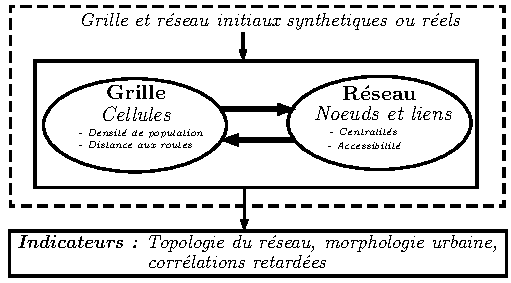
\includegraphics[width=\textwidth]{../../Figures/MesoCoEvol/mesocoevol_fr}

}




\sframe{Network Generation}{


At fixed time steps :

\begin{enumerate}
	\item Add new nodes preferentially to new population and connect them
	\item \justify Variable heuristic for new links, among: nothing, random, gravity-based deterministic breakdown, gravity-based random breakdown (from \cite{schmitt2014modelisation}), cost-benefits (from \cite{louf2013emergence}), biological network generation (based on \cite{tero2010rules})
\end{enumerate}

\medskip

\centering

%\frame{\includegraphics[height=0.31\textwidth]{figures/coevol_example-bio-process-1}}\hspace{0.2cm}
%\frame{\includegraphics[height=0.31\textwidth]{figures/coevol_example-bio-process-1-tick80}}
\includegraphics[width=0.8\linewidth]{../../Figures/Final/7-1-1-fig-networkgrowth-bioexample.jpg}


\footnotesize

\textit{Intermediate stage for biological network generation}

}






\sframe{Empirical Data : network indicators}{

\centering

%\includegraphics[width=0.53\textwidth]{figures/coevol_FR_indics_network_selected_2_discrquantiles}

\includegraphics[width=0.8\textwidth]{../../Figures/Final/4-1-2-fig-staticcorrs-network.jpg}



}



\sframe{Empirical Data : correlations}{

\centering

%\includegraphics[width=0.7\textwidth]{figures/coevol_FR_corr_PCA_rhoasize12}

\includegraphics[width=\textwidth]{../../Figures/Final/4-1-3-fig-staticcorrs-mapscorrs.jpg}

}



\sframe{Network Indicators}{

Network Topology measured by:

\begin{itemize}
	\item Betweenness and Closeness centralities: average and hierarchy
	\item Accessibility (weighted closeness)
	\item Efficiency (network pace relative to euclidian distance)
	\item Mean path length, diameter
\end{itemize}

}




\sframe{Model specification}{

\footnotesize

Patch utility given by $U_i = \sum_k w_k \cdot \tilde{x}_k$ with $\tilde{x}_k$ normalized local variables among population, betweenness and closeness centrality, distance to roads, accessibility ; aggregation done with probability $\left(U_i/\sum_k U_k\right)^\alpha$ ; diffusion among neighbors $n_d$ times with strength $\beta$

\medskip

\textbf{Network Generation :}

Adding a fixed number $n_N$ of new nodes : for patches such that $d_r < d_0$, probability to receive a node is

%%% note : not a proba for the last ? no pb as soon as in 0,1, realized anyway.

\[
p = P/P_{max} \cdot (d_M - d)/d_M \cdot \exp\left(-((d_r - d_0)/\sigma_r)^2\right)
\]

Nodes connected the shortest way to existing network.

\medskip

\textbf{General model parameters :}

\begin{itemize}
	\item Patch utility weights $w_k$
	\item General network generation parameters: growth time steps $t_N$, maximal additional links
\end{itemize}

}



\sframe{Deterministic breakdown Network generation}{

\begin{enumerate}
\item Gravity potential given by
\[
V_{ij}(d) = \left[ (1 - k_h) + k_h \cdot \left( \frac{P_i P_j}{P^2} \right)^{\gamma} \right]\cdot \exp{\left( -\frac{d}{r_g (1 + d/d_0)} \right)}
\]

\item $k\cdot N_L$ links are selected with lowest $V_{ij}(d_N)/V_{ij}(d_{ij})$, among which $N_L$ links with highest (lest costly) are realized
\item Network is planarized
\end{enumerate}
}


\sframe{Biological Network generation}{

Adding new links with biological heuristic:

\begin{enumerate}
	\item Create network of potential new links, with existing network and randomly sampled diagonal lattice
	\item Iterate for $k$ increasing ($k\in \{ 1,2,4 \}$ in practice) :
	\begin{itemize}
		\item Using population distribution, iterate $k\cdot n_b$ times the slime mould model to compute new link capacities
		\item Delete links with capacity under $\theta_d$
		\item Keep the largest connected component
	\end{itemize}
	\item Planarize and simplify final network
\end{enumerate}

}


\sframe{Model setup}{

\textbf{Synthetic setup: } rank-sized monocentric cities, simple connection with bord nodes to avoid bord effects 

\textbf{Real setup: } Population density raster at 500m resolution (European Union, from Eurostat)

\centering
\frame{\includegraphics[width=0.35\textwidth]{figuresraw/coevol_example_synthsetup}}\hspace{0.1cm}
\frame{\includegraphics[width=0.35\textwidth]{figuresraw/coevol_example-realsetup}}

\textbf{Stopping conditions: } fixed final time; fixed total population; fixed network size.

}








\sframe{Generated Urban Shapes: Urban Form}{

\centering

\frame{\includegraphics[width=0.28\textwidth]{figuresraw/coevol_example_synthsetup}}\hspace{0.1cm}
\frame{\includegraphics[width=0.28\textwidth]{figuresraw/coevol_example_form-accessonly}}\hspace{0.1cm}
\frame{\includegraphics[width=0.28\textwidth]{figuresraw/coevol_example_form-droadonly}}\\\vspace{0.1cm}
\frame{\includegraphics[width=0.28\textwidth]{figuresraw/coevol_example_form-bwonly}}\hspace{0.1cm}
\frame{\includegraphics[width=0.28\textwidth]{figuresraw/coevol_example_form-closenessonly}}\hspace{0.1cm}
\frame{\includegraphics[width=0.28\textwidth]{figuresraw/coevol_example_form-poponly}}

\footnotesize\textit{In order: setup; accessibility driven; road distance driven; betweenness driven; closeness driven; population driven.}

}





\sframe{Generated Urban Shapes: Network}{


\centering

%\frame{\includegraphics[width=0.28\textwidth]{figures/coevol_example_nw-connection}}\hspace{0.1cm}
%\frame{\includegraphics[width=0.28\textwidth]{figures/coevol_example_nw-random}}\hspace{0.1cm}
%\frame{\includegraphics[width=0.28\textwidth]{figures/coevol_example_nw-gravity}}\\\vspace{0.1cm}
%\frame{\includegraphics[width=0.28\textwidth]{figures/coevol_example_nw-rndbrkdwn}}\hspace{0.1cm}
%\frame{\includegraphics[width=0.28\textwidth]{figures/coevol_example_nw-cost}}\hspace{0.1cm}
%\frame{\includegraphics[width=0.28\textwidth]{figures/coevol_example_nw-bio}}

\includegraphics[width=\linewidth]{../../Figures/Final/7-1-2-fig-networkgrowth-examples.jpg}

\footnotesize\textit{In order: connection; random; deterministic breakdown; random breakdown; cost-driven; biological.}

}





\sframe{Results : Network Heuristics}{

\justify

\textit{Comparison of feasible space for network indicators with fixed density}

\bigskip

\includegraphics[width=0.52\textwidth,height=0.6\textheight]{figuresraw/coevol_feasible_space_withreal_pca_bymorph}
\includegraphics[width=0.43\textwidth,height=0.6\textheight]{figuresraw/coevol_distance_real_bymorph}



\footnotesize

\textit{(Left) Feasible spaces by morphological class and network heuristic; (Right) Distribution of distances to topologies of real networks}

}


\sframe{Results : Calibration}{

\justify

\vspace{-0.5cm}

Calibration (model explored with OpenMole~\cite{reuillon2013openmole}, $\sim 10^6$ model runs) at the first order on morphological and topological objectives, and on correlations matrices.

\bigskip

\begin{columns}
\column{0.4\textwidth}
\centering
\includegraphics[width=\textwidth]{figuresraw/coevol_pca_allobjs}
\column{0.2\textwidth}
\includegraphics[width=\textwidth]{figuresraw/coevol_pca_morpho_byheuristic}\\
\includegraphics[width=\textwidth]{figuresraw/coevol_pca_network_byheuristic}
\column{0.4\textwidth}
\includegraphics[width=\textwidth]{figuresraw/coevol_corrs-distrib_rhoasize4}

\end{columns}

\footnotesize\textit{(Left) Full indicator space; (Middle) Morphological and Topology, by network heuristic; (Right) Distance distribution for cumulated distance for indicators and correlations.}

}



\sframe{Calibration Method}{


\begin{itemize}
	\item Brute force exploration of a LHS sampling, 10 repetitions of the model for each parameter point.
	\item For each simulated point, closest in indicator space (euclidian distance for normalized indicators) among real points are selected.
	\item Among these, point with lowest distance to correlation matrix are taken.
\end{itemize}


}

\sframe{Calibration : optimal points}{

\centering

\includegraphics[width=0.45\textwidth]{figuresraw/coevol_dists_pareto_i1}
\includegraphics[width=0.45\textwidth]{figuresraw/coevol_dists_pareto_i10}

\footnotesize\textit{Pareto plots of distance to indicators and distance to correlation matrices, for a given simulated configuration and all real points.}

}



\sframe{Results : Causality Regimes}{

\textit{Unsupervised learning on lagged correlations between local variables unveils a diversity of causality regimes}

$\rightarrow$ Link between \emph{co-evolution regime} and morphogenetic properties of the urban system

\medskip

\centering

\includegraphics[width=0.52\textwidth,height=0.55\textheight]{figuresraw/coevol_centertrajs}
\includegraphics[width=0.4\textwidth,height=0.55\textheight]{figuresraw/coevol_cluster-params}

\footnotesize\textit{(Left) Lagged correlation profiles of cluster centers; (Right) Distribution of regimes across parameter space}

}






\sframe{Causality regimes: clustering}{

\centering

\includegraphics[width=0.48\textwidth]{figuresraw/coevol_clustcoef}
\includegraphics[width=0.48\textwidth]{figuresraw/coevol_diffclustcoef}

\medskip

\footnotesize\textit{Clustering coefficient (left) and its derivative (right) as a function of number of clusters}

}




\sframe{Discussion}{

\justify

\vspace{-1cm}

\textbf{Implications}

$\rightarrow$ This rather simple model reproduces most of existing urban forms in Europe for both population distribution and road network : which intrinsic dimension to the urban system and its morphological aspect ?

$\rightarrow$ Ability to reproduce static correlations and a variety of dynamical lagged correlation regimes suggests that the model captures some of the processes of co-evolution

%% implications for morphogenesis ?

\bigskip

\textbf{Developments}


$\rightarrow$ Towards a dynamical calibration ? Need of dynamical data

$\rightarrow$ Investigate the link between spatial non-stationarity and non-ergodicity through simulation by the model

$\rightarrow$ Compare network generation in a ``fair'' way (correcting for additional parameters, open question for models of simulation)


}
















%%%%%%%%%%%%%%%%%%%%
%%%% Network Morphogenesis


%\section*{Slime mould model}
% TODO Slime mould model


\sframe{Slime mold network morphogenesis model}{

Model studied by~\cite{tero2010rules} : exploration and reinforcement by a slime mould searching for ressources

\medskip

Settings :
\begin{itemize}
	\item Initial homogeneous network of tubes $ij$ of length $L_{ij}$, variable diameter $D_{ij}$, carrying a flow $Q_{ij}$.
	\item Nodes $i$ with a pressure $p_i$.
	\item $N$ nodes are origin/destination points : randomly at each step one becomes source $p_{i_+}=I_0$ and one other sink $p_{i_-}=-I_0$
\end{itemize}


}

\sframe{Network evolution}{

At each iteration :
\begin{enumerate}
	\item Determination of flows with Kirchoff's law (electrostatic analogy) : Ohm's law $Q_{ij}=\frac{D_{ij}}{L_{ij}}\cdot(p_{i}-p_{j})$ and conservation of flows $\sum_{j\rightarrow i}Q_{ij} = 0 , \sum_{j\rightarrow i_\pm}Q_{i_{\pm}j} = \pm I_0$
	\item Evolution of diameters ($\gamma$ reinforcement parameter) by
	\[
	\frac{dD_{ij}}{dt}=\frac{\left|Q_{ij}\right|^{\gamma}}{1+\left|Q_{ij}\right|^{\gamma}}-D_{ij}
	\]
\end{enumerate}

\medskip


$\rightarrow$ Extraction of the final network after convergence given a threshold parameter for diameters %(bimodal final distributions)

\medskip

$\rightarrow$ Multi-scale model : diameters are constant during an iteration to obtain equilibrium flows

}



\sframe{Indicators}{

Behavior of the model evaluated with performance indicators for generated network $(V_f,E_f)$, that are contradictory objectives :
          \bigskip
          \begin{itemize}
          \item Construction costs $c=\sum_{ij\in E_f}D_{ij}(t_f)$
          \bigskip
          \item \begin{justify}Average performance~\cite{banos2012towards}
          \[
          v=\frac{1}{|V_f|^2}\sum_{i,j\in V_f}\frac{d_{i\rightarrow j}}{||\vec{i}-\vec{j}||}
          \]
          \end{justify}
          \bigskip
          \item Robustness (\textit{Network Trip Robustness} index~\cite{sullivan2010identifying})
          \end{itemize}

}



\sframe{Example of networks}{
 \includegraphics[width=0.48\textwidth]{figuresraw/slimemould_networkDense}
 \hfill\includegraphics[width=0.48\textwidth]{figuresraw/slimemould_networkLessDense}\\
          \bigskip
 \justify
          \textit{Sensitivity of network topology to reinforcement coefficient $\gamma$. Left : $\gamma \sim 1$, robust network. Right : $\gamma >> 1$, arborescent network.}
}




\sframe{Sensitivity analysis}{
 
          \includegraphics[width=0.5\textwidth]{figuresraw/slimemould_graphe_cout}
          \includegraphics[width=0.5\textwidth]{figuresraw/slimemould_graphe_NTR}\\
          \bigskip
          \textit{Sensitivity of indicators to parameters $(N,I_0)$.}
      
}





\sframe{Application : Optimal transportation Corridor}{
          
Abstract application : \textit{Given a distribution of nodes to serve (sinks), what is the optimal corridor for an infrastructure at a larger scale (train or metro) for which stations are sources, in the sense of the multi-objective optimality of the local self-organized network ?}

\medskip
          
$\rightarrow$ Heuristic exploration of an arborescent set of potential infrastructures

\medskip

\includegraphics[width=0.48\textwidth]{figuresraw/slimemould_implantationtree}
\hfill \includegraphics[width=0.48\textwidth]{figuresraw/slimemould_ImplantationTreeview}
         	
%\textit{Heuristic tree to explore infrastructures.}
%\textit{Example of network generation for a given infrastructure.} 
          
}
          
          
          
\sframe{Pareto Optimisation}{
          
%\centering
\includegraphics[width=0.48\textwidth]{figuresraw/slimemould_implantationcntr}
\includegraphics[width=0.48\textwidth]{figuresraw/slimemould_implantationntrspeed}
          
\textit{Pareto optimisation : projection of explored configurations in indicator space to obtain the Pareto front.}          
}

\sframe{Pareto Optimisation}{

\centering
  \includegraphics[width=0.8\textwidth]{figuresraw/slimemould_paretosimplantation}

\medskip

\textit{Configurations corresponding to three optimal points.}

}


\sframe{Application : Optimal Network Design}{

\footnotesize

$\rightarrow$ Mission of prospective for Romainville city : itinary of an intra-urban shuttle with imposed stops.

\medskip

$\rightarrow$ NP-hard problem similar to a Travelling Salesman Problem, but multi-objective (cost, speed, robustness). The bottom-up network generation applied on the initial street network gives a compromise solution.

\includegraphics[width=0.32\columnwidth]{figuresraw/slimemould_tick1}
\includegraphics[width=0.32\columnwidth]{figuresraw/slimemould_tick10}
\includegraphics[width=0.32\columnwidth]{figuresraw/slimemould_tick20}\\
\includegraphics[width=0.32\columnwidth]{figuresraw/slimemould_tick50}
\includegraphics[width=0.32\columnwidth]{figuresraw/slimemould_tick101}
\includegraphics[width=0.32\columnwidth]{figuresraw/slimemould_reseauFinal}\\

\textit{Progressive convergence of the network towards an optimal network connecting the fixed points (in red), starting from the initial street network.}

}




%%%%%%%%%%%%%%%%%%
%\section*{Quantitative Epistemology}
% TODO Quantitative Epistemology



\sframe{Citation Network}{
\centering
%%\vspace{-0.5cm}
\includegraphics[height=0.9\textheight]{../../Figures/Final/2-2-2-fig-quantepistemo-citnw.jpg}

}


\sframe{Citation Network Properties}{

For the core (hence full) subnetwork :

\begin{itemize}
	\item Size $V=3510$, Mean degree $\bar{d}=2.53$ and density $\gamma=0.0013$, weakly connected.
	\item 13 communities, directed modularity~\cite{nicosia2009extending} 0.66 (null model gives $0.0005 \pm 0.0051$ on $N=100$ bootstraps)
	\item Content : LUTI (18\%), Urban and Transportation Geography (16\%), Infrastructure Planning (12\%), TOD (6\%), Spatial Networks (17\%), Accessibility studies (18\%)
\end{itemize}

}



\sframe{Semantic Network}{
\centering
%%\vspace{-0.5cm}
\includegraphics[height=\textheight]{../../Figures/Final/A-quantepistemo-semanticnw.jpg}
}


\sframe{Semantic communities}{

\footnotesize
\vspace{-0.8cm}
\begin{table}
\label{tab:quantepistemo:semanticdomains}
\begin{tabular}{llll}
\hline\noalign{\smallskip}
Name & Size & Weight & Keywords  \\
\noalign{\smallskip}\hline\noalign{\smallskip}
Networks & 820 & 13.57\% & \texttt{social network, spatial network, resili} \\
Policy & 700 & 11.8\% & \texttt{actor, decision-mak, societi} \\
Socio-economic & 793 & 11.6\% & \texttt{neighborhood, incom, live} \\
High Speed Rail & 476 & 7.14\% & \texttt{high-spe, corridor, hsr} \\
French Geography & 210 & 6.08\% & \texttt{système, développement, territoire} \\
Education & 374 & 5.43\% & \texttt{school, student, collabor} \\
Climate Change & 411 & 5.42\% & \texttt{mitig, carbon, consumpt} \\
Remote Sensing & 405 & 4.65\% & \texttt{classif, detect, cover} \\
Sustainable Transport & 370 & 4.38\% & \texttt{sustain urban, travel demand, activity-bas} \\
Traffic & 368 & 4.23\% & \texttt{traffic congest, cbd, capit} \\
Maritime Networks & 402 & 4.2\% & \texttt{govern model, seaport, port author} \\
Environment & 289 & 3.79\% & \texttt{ecosystem servic, regul, settlement} \\
Accessibility & 260 & 3.23\% & \texttt{access measur, transport access, urban growth} \\
Agent-based Modeling & 192 & 3.18\% & \texttt{agent-bas, spread, heterogen} \\
Transportation planning & 192 & 3.18\% & \texttt{transport project, option, cba} \\
Mobility Data Mining & 168 & 2.49\% & \texttt{human mobil, movement, mobil phone} \\
Health Geography & 196 & 2.49\% & \texttt{healthcar, inequ, exclus} \\
Freight and Logistics & 239 & 2.06\% & \texttt{freight transport, citi logist, modal} \\
%%Spanish Geography & 106 & 1.26\% & \texttt{movilidad urbana, criteria, para} \\
Measuring & 166 & 1.0\% & \texttt{score, sampl, metric} \\
\noalign{\smallskip}\hline
\end{tabular}
\end{table}
%%%%%%%%%%%%%%%%%%%


}




\sframe{Interdisciplinarity patterns}{


\centering

\includegraphics[width=\textwidth]{../../Figures/Final/2-2-2-fig-quantepistemo-interdisc.jpg}


\footnotesize

\textit{Measures of interdisciplinarities}


}









%
%%%%%%%%%%%%%%%%%%
%\section*{Causality Regimes}
% TODO Causality Regimes


\sframe{Effet structurants des infrastructures}{


\justify

\textit{De \cite{bonnafous1974methodologies} à \cite{offner1993effets} : quels effets de structure des infrastructures de transport sur les territoires ?}

\bigskip
\bigskip

$\rightarrow$ Existence de processus co-évolutifs \cite{bretagnolletel00459720}

\medskip

$\rightarrow$ A petite échelle et sur le temps long, existence de dynamiques structurelles des systèmes urbains \cite{espacegeo2014effets}

\medskip

$\rightarrow$ La question des causalités circulaires revient à toutes les échelles (e.g. échelle métropolitaine et mobilité \cite{cerqueira2017inegalites}) et dans différents domaines (retombées locales et innovation \cite{audretsch1996r})



}




\sframe{Causalité en Géographie}{

\justify

$\rightarrow$ La Géographie classique s'intéressait déjà à des liens causaux dans l'espace \cite{loi1985etude}

\bigskip

$\rightarrow$ \cite{claval1985causalite} : au delà de la causalité réductionniste en analyse systémique

\bigskip

$\rightarrow$ La systèmogenèse introduite par \cite{durand2003geographes} se concentre sur la dynamique et les dépendances au chemin

\bigskip

$\rightarrow$ Vers une approche complexe de la causalité ? \cite{morin1976methode}

}


\sframe{Approches empiriques existantes}{

\justify

\textbf{Réseaux de transports et territoires}

\begin{itemize}
	\item\justify Corrélations retardées : \cite{levinson2008density} Population et connectivité au réseau à Londres ; \cite{doi10.1068/b39089} données historiques en Italie du Nord
\end{itemize}
\begin{itemize}
	\item\justify Variables instrumentales : \cite{duranton2012urban} Réseau routier et emplois aux Etats-Unis ; \cite{berger2017locomotives} effet significatif du réseau ferré suédois sur les trajectoires urbaines
\end{itemize}


\medskip

\textbf{Corrélations spatio-temporelles}

\begin{itemize}
	\item Méthode de correspondance pour les flux de trafic \cite{liu2011discovering}
	\item Causalité de Granger généralisée en neurosciences \cite{ke2007spatio}
	\item Corrélations spatio-temporelles en Vision par Ordinateur \cite{ke2007spatio}
\end{itemize}



}




\sframe{Aperçu de la méthode}{

\centering

\includegraphics[width=\linewidth]{../../Figures/Theory/causality_regimes}

}



\sframe{Formalisation de la méthode}{

Estimateur de corrélation $\hat{\rho}$ s'appliquant dans le temps, l'espace, et les répétitions, i.e. la covariance est estimée par $\hat{\Cov}\left[X,Y\right] = \hat{\mathbb{E}}_{i,t,k}\left[XY\right] - \hat{\mathbb{E}}_{i,t,k}\left[X\right]\hat{\mathbb{E}}_{i,t,k}\left[Y\right]$

\bigskip

Corrélations retardées définies comme

\begin{equation}
\rho_{\tau}\left[X_{j_1},X_{j_2}\right] = \hat{\rho}\left[x^{(k)}_{i,j_1,t - \tau},x^{(k)}_{i,j_2,t}\right]
\end{equation}

\bigskip

Le motifs de $\textrm{argmax}_{\tau} \rho_{\tau}\left[X_{j_1},X_{j_2}\right]$ ou de $\textrm{argmin}_{\tau} \rho_{\tau}\left[X_{j_1},X_{j_2}\right]$ (en les supposant clairement définis : e.g. significativité statistique, valeur seuil) capture le sens de la causalité entre $j_1$ et $j_2$

\medskip

$\rightarrow$ Datamining sur $\rho_\tau$ (possiblement paramétré comme $\rho_\tau^{(\omega)}$) pour explorer les motifs de causalité.

}



\sframe{Illustration pour 2 variables}{

\centering

\includegraphics[height=0.9\textheight]{../../Figures/Theory/causality_twovars.pdf}

}



\sframe{Validation basique}{

\includegraphics[width=\linewidth]{../../Figures/Final/4-2-2-fig-causalityregimes-arma.jpg}

\medskip

\textit{Données synthétiques : processus AR avec retard 2, termes croisés paramétrés par $(a_1,a_2) \in [-0.1,0.1]$ aléatoires.}

}






\sframe{Validation sur données synthétiques}{

% present strategy and rbd model

\includegraphics[width=0.32\textwidth]{figuresraw/ex_60_wdens0_wroad1_wcenter1_seed272727}\hspace{0.1cm}
\includegraphics[width=0.32\textwidth]{figuresraw/ex_60_wdens1_wroad1_wcenter0_seed272727}\hspace{0.1cm}
\includegraphics[width=0.32\textwidth]{figuresraw/ex_60_wdens1_wroad1_wcenter1_seed272727}\hspace{0.1cm}

\medskip

\textit{Configurations urbaines synthétiques générées par un modèle de morphogenèse hybride issu de \cite{raimbault2014hybrid}}

}


\sframe{Description du modèle de morphogenèse}{

% plus de details sur le rbd
\begin{itemize}
\item Automate cellulaire: cellules d'une grille carrée $(L_{i,j})_{1\leq i,j\leq N}$
, occupées ou non (fonction \textrm{$\ensuremath{\delta(i,j,t)\in\{0,1\}}$)}
\end{itemize}
\vfill{}

\begin{itemize}
\item Réseau vectoriel $G(t)=(V(t),E(t))$ qui évolue,
incluant des centres urbains fixes $C_{0}\subset V(0)$ auxquels des activités
$a\in\{1,\ldots,a_{max}\}$ sont attribuées (propriétés fonctionnelles de l'environnement urbain).
\end{itemize}
\vfill{}

\begin{itemize}
\item Variables explicatives $(d_{k})_{1\leq k\leq K}$ définies sur les cellules, avec des poids associés $(\alpha_{k})_{1\leq k\leq K}$
(paramètres principaux du modèle), qui sont:

\begin{itemize}
\item $d_{1}$ densité autour de la cellule (dans un rayon fixé $r$)
\item $d_{2}$ distance à la route la plus proche
\item $d_{3}$ distance au centre le plus proche par le réseau
\item \textrm{$d_{4}(i,j,t)=\left(\frac{1}{a_{\max}}\sum_{a=1}^{a_{\max}}d_{3}(i,j,t;a)^{p_{4}}\right)^{1/p_{4}}$
}: accessibilité intégrée aux activités
\end{itemize}
\end{itemize}
\vfill{}


}



\sframe{Règles d'évolution}{

A chaque pas de temps :\vfill{}

\begin{itemize}
\item Etalement de la surface occupée : les meilleures $N$ cellules selon
la valeur du potentiel $v(i,j,t)=\frac{1}{\sum_{k}\alpha_{k}}\sum_{k=1}^{K}\alpha_{k}\;\frac{d_{k,\max}(t)-d_{k}(i,j,t)}{d_{k,\max}(t)-d_{k,\min}(t)}$
sont construites.\vfill{}

\item Adaptation du réseau : quand une nouvelle cellule est construite, si $d_{2}>\theta_{2}$, la cellule est connectée au réseau par une route directe.\vfill{}

\end{itemize}
}




\sframe{Profils de corrélations retardées}{

\includegraphics[width=\textwidth]{figuresraw/regimes_1.png}

%\textit{Values of $\rho_{\tau}$ for all couples of three explicative variables (density, distance to center, distance to roads), for 8 extreme parameter points}

}





\sframe{Profils de corrélations retardées}{

\includegraphics[width=\textwidth]{figuresraw/regimes_2.png}

}




\sframe{Régimes endogènes de causalité}{

Exploration intensive de l'espace des paramètres du modèle (1000 points de paramètres x 100 répétitions) avec le logiciel OpenMole \cite{reuillon2013openmole}

\medskip

\includegraphics[width=0.52\textwidth]{figuresraw/dccoef-knum_valuesFALSEtheta05-3}
\includegraphics[width=0.44\textwidth]{figuresraw/clusters-PCA-features_valuesFALSEtheta2_k6}

\footnotesize\textit{Classification non-supervisée (\textit{k-means} robustes) sur les caractéristiques $\tau_{min},\tau_{max}$ : (Gauche) Dérivée du coefficient de clustering en fonction du nombre de clusters $k$; (Droite) Visualisation en plan principal pour $k=6$.}

}



\sframe{Composition des régimes}{

\centering

\includegraphics[width=\textwidth]{../../Figures/CausalityRegimes/clusters-centertrajs-facetclust_valuesFALSEtheta2_k6}

\textit{Valeurs des centres des clusters en termes de $\rho_{\tau}$}

}


\sframe{Interprétation des régimes}{

\centering

\includegraphics[width=0.9\textwidth]{../../Figures/CausalityRegimes/clusters-paramfacet_valuesFALSEtheta2_k6}

\textit{Position des clusters dans l'espace des paramètres $w_i$}


}




\sframe{Application: Cas d'étude}{
\centering

\includegraphics[width=0.8\textwidth]{../../Figures/Final/1-2-1-fig-casestudies-projects.jpg}

\medskip

\textit{Projet de transport successifs pour la nouvelle infrastructure de transport du Grand Paris}

}






\sframe{Application: Résultats}{


\centering

\includegraphics[width=0.62\textwidth]{../../Figures/Final/1-2-1-fig-casestudies-empiricalres}

\textit{Valeurs de $\rho_{\tau}$ pour les différents projets (colonnes) et les différentes variables (lignes), avec les différentiels d'accessibilité}

}






%%% application to south africa


\sframe{Application to South Africa: Network Analysis}{

\textit{Evolution of Network measures : anomalous trend rupture in centralities}

\medskip

\centering

%\includegraphics[width=0.4\textwidth]{figures/southafrica_nw_nwSize}
%\includegraphics[width=0.45\textwidth]{figures/southafrica_nw_meanCentralities}\\
%\includegraphics[width=0.4\textwidth]{figures/southafrica_nw_efficiency}
%\includegraphics[width=0.45\textwidth]{figures/southafrica_nw_hierarchies}


\includegraphics[width=\textwidth]{../../Figures/Final/4-2-3-fig-causalityregimes-network.jpg}

}




\sframe{Application à l'Afrique du Sud}{

\centering

\includegraphics[width=0.5\textwidth]{figuresraw/southafrica_meanabscorrs}
\includegraphics[width=0.5\textwidth]{figuresraw/southafrica_significantcorrs}

\medskip

\textit{Détermination de la fenêtre temporelle et de la portée spatiale de l'accessibilité}


}


\sframe{Application à l'Afrique du Sud}{


\centering

\includegraphics[width=0.82\textwidth]{../../Figures/Final/4-2-3-fig-causalityregimes-sudafcorrs.jpg}

\medskip

\textit{Inversion du sens de la causalité suggère un effet de ségrégation structurelle des politiques d'apartheid}



}



\sframe{Application à la France}{

\centering

\includegraphics[width=0.5\textwidth]{figuresraw/significantcorrs_d0}
\includegraphics[width=0.5\textwidth]{figuresraw/significantcorrs_Tw}

\medskip

\textit{Fenêtre temporelle et portée spatiale optimales (réseau ferré et population sur la période 1830-1999)}

}

\sframe{Application à la France}{


\centering

\includegraphics[width=0.82\textwidth]{figuresraw/laggedCorrs_time_Tw4}

\textit{Profils de corrélation : pas de signal significatif}

}



\sframe{Discussion}{

\justify

\vspace{-1cm}

\textbf{Implications}

$\rightarrow$ Motifs de corrélations retardées pour identifier des ``effets structurants'' dans des systèmes complexes

\medskip

$\rightarrow$ Le concept opérationnel de \textit{Régime de causalité} introduit une nouvelle façon de comprendre la co-évolution dans les modèles de simulation

\bigskip

\textbf{Développements}

$\rightarrow$ Caractérisation de la diffusion spatio-temporelle : test de l'hypothèse de la diffusion spatiale de l'innovation dans la Théorie Evolutive des Villes \cite{pumain2010theorie}

\medskip

$\rightarrow$ Echelles optimales pour la stationnarité : lien avec GWR

\cite{brunsdon1998geographically}

}


\sframe{Granger causality}{

Granger causality test based on VAR processes :

\[
X(t) = \sum_{0 \leq \tau \leq \tau_Y} b_{\tau} Y(t - \tau)
\]

\bigskip

If there exists $b_{\tau}$ such that $\left|b_{\tau}\right|> 0$ significantly, then $Y$ Granger-causes $X$.

\bigskip

We have then $\rho_{\tau}(Y,X) > 0$.


}










%
%
%%%%%%%%%%%%%%%%%%
%\section*{Interaction Gibrat}
% TODO Interaction Gibrat



%% Interaction Gibrat


\sframe{Macroscopic Interaction Model Rationale}{

\justify

%% bit of theory

\textbf{Rationale :} extend an interaction model for system of cities by including physical network as an additional carrier of spatial interactions

\bigskip

$\rightarrow$ Work under Gibrat independence assumptions, i.e. $\Covb{P_i(t)}{P_j(t)}=0$. If $\vec{P}(t+1)=\mathbf{R}\cdot \vec{P}(t)$ where $\mathbf{R}$ is also independent, then $\Eb{\vec{P}(t+1)}=\Eb{\mathbf{R}}\cdot\Eb{\vec{P}}(t)$. Consider expectancies only (higher moments computable similarly)

\medskip

$\rightarrow$ With $\vec{\mu}(t)=\Eb{\vec{P}(t)}$, we generalize this approach by taking $\vec{\mu}(t+1)=f(\vec{\mu}(t))$


}


\sframe{Macroscopic Model Formulation}{

Let $\vec{\mu}(t)=\Eb{\vec{P}(t)}$ cities population and $(d_{ij})$ distance matrix


\medskip

Model specified by

\[
f(\vec{\mu}) = r_0\cdot \mathbf{Id}\cdot \vec{\mu} + \mathbf{G}\cdot \mathbf{1} + \mathbf{N}
\]

 with 
\begin{itemize}
\item $G_{ij} = w_G\cdot \frac{V_{ij}}{<V_{ij}>}$ and $V_{ij} = \left(\frac{\mu_i\mu_j}{\sum{\mu_k}^2}\right)^{\gamma_G} \exp{(-d_{ij}/d_G)}$
\item $N_{i} = w_N \cdot \sum_{kl} \left(\frac{\mu_k\mu_l}{\sum\mu}\right)^{\gamma_N}\exp{(-d_{kl,i})/d_N}$ where $d_{kl,i}$ is distance to shortest path between $k,l$ computed with slope impedance ($Z=\left(1+\alpha/\alpha_0\right)^{n_0}$ with $\alpha_0\simeq 3$)
\end{itemize}



}


\sframe{Data : stylized facts}{


Population data for French-cities (Pumain-INED database : 1831-1999)

%% correlation curves, non-stationarity of network effects

\medskip

\textit{Non-stationarity of log-returns correlations function of distance}

\centering

\includegraphics[width=0.8\textwidth,height=0.7\textheight]{../../Figures/Final/4-3-2-fig-interactiongibrat-ts-correlations.jpg}

}


\sframe{Geographic abstract network}{

%% computation of geo shortest paths

\textit{Physical transportation network abstracted through a geographical shortest path network}

%% map with shortest path examples

\medskip

\centering

\includegraphics[height=0.75\textheight]{../../Figures/Final/4-3-2-fig-interactiongibrat-interface.jpg}

}

\sframe{Results : model exploration}{

%% network effects graphs


\textit{Evidence of physical network effects : fit improve through feedback at fixed gravity}

\medskip

\centering

\includegraphics[width=\textwidth]{../../Figures/Final/4-3-2-fig-interactiongibrat-networkeffects.jpg}

}



\sframe{Results : model calibration}{

% ga calibration, both full model and gravity only

Model calibration using GA on computation grid, with software \texttt{OpenMole}~\cite{reuillon2013openmole}

\bigskip

\textit{Pareto front for full model calibration, objectives MSE and MSE on logs}

\medskip

\includegraphics[width=\textwidth,height=0.65\textheight]{../../Figures/Final/4-3-2-fig-interactiongibrat-gravity-pareto.jpg}

}



\sframe{Results : non-stationary gravity model calibration}{

%% calibration on periods

\includegraphics[width=\textwidth,height=0.8\textheight]{../../Figures/Final/4-3-2-fig-interactiongibrat-gravity-params.jpg}

}


\sframe{Results : non-stationary full model calibration}{

%% calibration on periods

\includegraphics[width=\textwidth,height=0.8\textheight]{../../Figures/Final/4-3-2-fig-interactiongibrat-feedback.jpg}

}



\sframe{Quantifying overfitting : Empirical AIC}{

\justify

\vspace{-0.5cm}

\textit{Not clear nor well theorized how to deal with overfitting in models of simulation.} \textbf{Intuitive idea : } Approximate gain of information by approaching models of simulation by statistical models.

\medskip

Let $M_k^{\ast} = M_k\left[\alpha_k^{\ast}\right]$ computational models heuristically fitted to the same dataset. With $S_k \simeq M_k^{\ast}$, we suppose that $\Delta D_{KL}\left( M_k^{\ast},M_{k'}^{\ast}\right) \simeq \Delta D_{KL}\left( S_k,S_{k'}\right)$ if fits of $S_k$ are negligible compared to fit difference between computational models and models have same parameter number.


\bigskip

\textbf{Application} $M_1$ : gravity only model with $(r_0=0.0133,w_G=1.28e-4,\gamma_G=3.82,d_G=4e12)$ ; $M_2$ : full model with $(r_0=0.0128,w_G=1.30e-4,\gamma_G=3.80,d_G=8.4e14,w_N=0.603,\gamma_N=1.148,d_N=7.474)$

%%Fitting of independent polynomial models ($\tilde{P}_i(t) = Q\left[\tilde{P}_i(t-1)\right]$) with 4 and 7 parameters) gives $\Delta D_{KL} \simeq 19.7$ $\rightarrow$ fit improvement without overfitting



}





\sframe{Empirical AIC values}{

\begin{table}[ht]
\caption{Empirical AIC results.}
\begin{tabular}{|l|l|l|l|l|l}
%%\hrule
Modèle Statistique &$M^{(1)}$ &$M^{(2)}$ & $\Delta AIC$ & $\Delta BIC$\\
%%\hrule
Polynomial & 0.01438 & 0.01415 & 19.59 & 3.65\\
Log-polynomial & 0.01565  & 0.01435 & 125.37 & 109.43\\
Polynomial Généralisé & 0.01415  & 0.01399 & 11.70 & -4.23\\
%%\hrule
\end{tabular}
\end{table}


}


%
%
%
%%%%%%%%%%%%%%%
%\section*{Macroscopic co-evolution}
% Macroscopic co-evolution


%
%

\sframe{Generic Model}{
%
%% idea : present it with a schema : YES.
%
\centering

\includegraphics[width=\textwidth]{../../Figures/MacroCoEvol/model.pdf}

}

%
%
%
%
%


\sframe{Model Formalization : Network Growth}{

Given the flow $\phi$ in a link, its effective distance is updated following

\begin{enumerate}
\item For the thresholded case
\[
d(t+1) = d(t)\cdot \left( 1 + g_{max} \cdot \left[\frac{1 - \left(\frac{\phi}{\phi_0}\right)^{\gamma_s}}{1 + \left(\frac{\phi}{\phi_0}\right)^{\gamma_s}}\right]\right)
\]
\item For the full growth case
\[
d(t+1) = d(t)\cdot \left(1 + g_{max} \cdot \left[\frac{\phi}{\max \phi}\right]^{\gamma_s}\right)
\]
\end{enumerate}

where $\gamma_s$ is a hierarchy parameter, $\phi_0$ a threshold parameter and $g_{max}$ the maximal growth rate easily adjustable to realistic values by computing $(1+g_{max})^{t_f}$
%
%
%


}


%
%


\sframe{Model Formalization : Indicators}{
  \begin{itemize}
  \item Hierarchy, Entropy, Summary statistics in time
  \item Initial-final rank correlation (changes in the hierarchy) for variable $X$ : $\rho\left[X_i(t=0),X_i(t=t_f)\right]$
  \item Trajectory diversity for variable $X$ : with $\tilde{X}_i(t)\in \left[0;1\right]$ rescaled trajectories,
  \[
    \frac{2}{N\cdot(N-1)}\sum_{i<j} \left(\frac{1}{T}\int_{t} \left(\tilde{X}_i(t) - \tilde{X}_j(t)\right)^2 \right)^{\frac{1}{2}}
  \]
  \item Average trajectory complexity (number of inflexion points)
  \item Pearson correlations conditionally to distance $\hat{\rho}_d\left[(X(\vec{x}_1,Y(\vec{x}_2))|||\vec{x}_1-\vec{x}_2||\sim d\right]$
  \item Lagged return correlations $\hat{\rho}_{\tau}\left[\Delta X(t),\Delta Y(t-\tau)\right]$ (Granger causality)
  \end{itemize}
}


%
%


\sframe{Model Specification : Abstract Network}{
 % description + illustration (t0, tf)
 
\textit{Complete virtual network between cities, initialized with euclidian distances ; thresholded reinforcement of speeds as a function of flows.}
 
 \bigskip
 
 \centering
 
 \includegraphics[width=0.4\textwidth]{figuresraw/macrocoevol_example_virtual_0_t0}\hspace{0.2cm}
 \includegraphics[width=0.4\textwidth]{figuresraw/macrocoevol_example_virtual_0_tf}
 
 {\small\textit{Exemple of run ($t_f=30$). Level of red gives overall growth and link width flows.}}
 
}





\sframe{Model Behavior}{
%
%\includegraphics[width=0.48\linewidth]{figures/macrocoevol_closenessSummaries_mean_gravityWeight0_001}
%\includegraphics[width=0.48\linewidth]{figures/macrocoevol_populationEntropies_gravityWeight0_001}\\
%\includegraphics[width=0.48\linewidth]{figures/macrocoevol_complexityAccessibility_synthrankSize1_nwGmax0_05}
%\includegraphics[width=0.48\linewidth]{figures/macrocoevol_rankCorrAccessibility_synthrankSize1_nwGmax0_05}
%

\includegraphics[height=\textheight]{../../Figures/Final/6-2-2-fig-macrocoevol-behavior-aggreg.jpg}

}

%
%

% -- NOT NEEDED : regimes already in main slide --
%\sframe{Correlation Patterns}{
%
%\includegraphics[width=0.48\linewidth]{figures/macrocoevol_distcorrs_gravityWeight5e-04_nwThreshold4_5}
%\includegraphics[width=0.48\linewidth]{figures/macrocoevol_laggedcorrs_gravityWeight5e-04_nwThreshold4_5}
%
%\centering

%\includegraphics[width=\linewidth]{../../Figures/Final/6-1-3-fig-macrocoevolexplo-correlations.jpg}
%}




\sframe{Calibration}{

%\includegraphics[width=0.48\linewidth]{figures/macrocoevol_pareto_gravityDecay}
%	\includegraphics[width=0.48\linewidth]{figures/macrocoevol_pareto_nwThreshold}

\centering

\includegraphics[width=\linewidth]{../../Figures/Final/6-2-3-fig-macrocoevol-pareto.jpg}


}


%
%
\sframe{Calibration: Parameters}{


%
%\includegraphics[width=0.32\linewidth]{figures/macrocoevol_param_gravityWeight_filt1}
%	\includegraphics[width=0.32\linewidth]{figures/macrocoevol_param_gravityDecay_filt1}
%	\includegraphics[width=0.32\linewidth]{figures/macrocoevol_param_gravityGamma_filt1}\\
%	\includegraphics[width=0.32\linewidth]{figures/macrocoevol_param_nwExponent_filt1}
%	\includegraphics[width=0.32\linewidth]{figures/macrocoevol_param_nwThreshold_filt1}
%	\includegraphics[width=0.32\linewidth]{figures/macrocoevol_param_nwGmax_filt1}
%

\centering

\includegraphics[width=\linewidth]{../../Figures/Final/6-2-3-fig-macrocoevol-parameters.jpg}



}






\sframe{Model Specification: Physical Network}{
 
 \textit{Physical initial network with uniform speeds ; reinforcement of speeds as a function of flows.}
 
 \medskip
 
 \centering
 
% \includegraphics[width=\textwidth]{../../Figures/macrocoevol_example_slimemould_1_t0}\hspace{0.2cm}
% \includegraphics[width=0.4\textwidth]{figures/macrocoevol_example_slimemould_1_tf}
 \includegraphics[width=\linewidth]{../../Figures/Final/6-2-3-fig-macrocoevol-slimemould.jpg}
 
 
 \medskip
 
 % emergence of hierarchy : find results of (Baptiste, 99), somehow similar.

$\rightarrow$ \textit{Emergence of a hierarchical transportation network. Full behavior still to be explored.}

}






%%%%%%%%
%% LUTECIA


%%%%%%%%%%%%%%%%%%%
%\section*{Transportation Governance}
% TODO Transportation Governance



\sframe{The LUTECIA Model : Rationale}{

\justify


Towards a more complex approach to network growth rules ? $\rightarrow$ a co-evolution approach including transportation governance

\medskip

\textit{Mega-city Regions~\cite{hall2006polycentric} exhibit new qualitative regimes of urban systems ?}

\bigskip

$\rightarrow$ A LUTI + infrastructure provision model (LUTECIA)

\medskip

$\rightarrow$ Coevolution transport / urbanism (LUTI model with endogeneous transport infrastructure provision)

\medskip

$\rightarrow$ Game theory framework to predict emergence of centralized decision within a polycentric region

\medskip

$\rightarrow$ Importance of accessibility at MCR scale

}



\sframe{The LUTECIA Model : Structure}{

LU : Land Use module ; T : Transport module ; EC : Evaluation of Centralized decision module ; I : Infrastructure provision module ; A : Agglomeration economies module

\medskip

\includegraphics[width=\textwidth]{figuresraw/lutetia_structure}

}


\sframe{Governance Modeling}{

Matrix of actors utilities, depending on respective choices

\bigskip

\begin{tabular}{ |c|c|c| } 
 \hline
 0 $|$ 1  & C & NC \\ \hline
 C & $U_i = \kappa \cdot \Delta X_i(Z^{\ast}_C) - I - \frac{J}{2}$
   & $\begin{cases}U_0 = \kappa \cdot \Delta X_0(Z^{\ast}_0)-I \\U_1 = \kappa \cdot \Delta X_1(Z^{\ast}_1)-I - \frac{J}{2}\end{cases}$ \\ \hline
 NC & $\begin{cases}U_0 = \kappa \cdot \Delta X_0(Z^{\ast}_0)-I - \frac{J}{2}\\U_1 = \kappa \cdot \Delta X_1(Z^{\ast}_1)-I\end{cases}$
   & $U_i = \kappa \cdot \Delta X_i(Z^{\ast}_i) - I$ \\
 \hline
\end{tabular}


\bigskip

Two types of games implemented :
\begin{itemize}
\item Mixed Nash equilibrium, where actors compete
\item One Rational Discrete Choice equilibrium
\end{itemize}


}




\sframe{Lutecia model parameters}{

\begin{center}
\begin{tabular}{|c|c|c|}%c|c|c|}
  \hline
 Sub-model & Parameter & Name\\% & Process & Domain & Default\\
  \hline
\multirow{5}{*}{Land-use}& $\lambda$ & Accessibility range \\\cline{2-3}% & Accessibility & $]0;1]$ & $0.001$ \\\cline{2-6}
 & $\gamma_A$ & Cobb-Douglas exponents actives\\\cline{2-3}% & \multirow{2}{*}{Utility} & $[0;1]$ & $0.85$ \\\cline{2-3}\cline{5-6}
 & $\gamma_E$ & Cobb-Douglas exponents employments \\\cline{2-3}%&  & $[0;1]$ & $0.85$ \\\cline{2-6}
 & $\beta$ & Discrete choices exponent \\\cline{2-3}%& \multirow{2}{*}{Relocalization} & $[0;+\infty]$ & $1$ \\\cline{2-3}\cline{5-6}
 & $\alpha$ & Relocation rate \\\hline%&  & $[0;1]$ & $0.05$ \\\hline
Transport & $v_G$ & Network speed \\\hline%& Hierarchy & $[1;+\infty [$ & $5$ \\\hline
\multirow{2}{*}{Governance} & $J$ & Collaboration cost\\\cline{2-3}% & \multirow{2}{*}{Planning} & $[0;0.005]$ & $0.001$ \\\cline{2-3}\cline{5-6}
 & $l_r$ & Infrastructure length \\\hline%&  & $]0;\sqrt{2}\cdot K [$ & $2$ \\\hline
\end{tabular}
\end{center}

}



\sframe{Model Output : Examples}{

\textbf{Implementation :} Netlogo ; particular treatment for dynamical programming computation of network shortest distances. Exploration with High Performance Computing on grid with \texttt{OpenMole}~\cite{reuillon2013openmole}

\medskip

\centering

\includegraphics[width=\textwidth,height=0.7\textheight]{figuresraw/lutetia_exrun}

}


\sframe{Land-use dynamics}{

\textit{Lessons from systematic exploration of the land-use module:}

\begin{itemize}
	\item Large diversity of morphological trajectories in time for varying $\gamma_A, \gamma_E, \lambda, \beta$
	\item Diversity of final forms obtained
	\item It is possible to minimize, at fixed $\alpha = 1$, the total quantity of relocalization
\end{itemize}

\begin{center}
\includegraphics[width=0.45\textwidth]{../../Figures/Final/A-lutecia-morphosens.jpg}
\includegraphics[width=0.3\textwidth]{../../Figures/Final/A-lutecia-morphotrajs.jpg}
\end{center}

}






\sframe{Model Exploration}{

\textit{Influence of governance parameters on network topology}

\medskip
\centering

\includegraphics[height=0.8\textheight]{../../Figures/Final/7-3-3-fig-lutecia-governance.jpg}

}

\sframe{Model Application}{


\textit{Stylized application to the Pear River Delta Mega-city Region}

\medskip

\centering

\includegraphics[width=\textwidth]{../../Figures/Final/7-3-3-fig-lutecia-ex-prd.jpg}

}


\sframe{Model Application: target networks}{


\textit{Different calibration setup: current and planned network}

\medskip

\centering

\includegraphics[width=\textwidth]{../../Figures/Final/A-lutecia-realsetup.jpg}

}





\sframe{Model Calibration}{

\textit{Calibration on the generated network (fixed land-use)}

\medskip

\centering

\includegraphics[height=0.8\textheight]{../../Figures/Final/7-3-3-fig-lutecia-calib.jpg}

}


\sframe{Effects of co-evolution}{

\textit{Unveiling the coupling between urban development and transportation networks}

\medskip

\centering

\includegraphics[height=0.8\textheight]{../../Figures/Final/7-3-3-fig-lutecia-coevol.jpg}

}






%%%%%%%%
% other perspectives : traffic flows ; energy price



%\section*{Traffic flow analysis}
% Traffic flow analysis


\sframe{Traffic Modeling : User Equilibrium Frameworks}{

\justify

% from static user eq to recent theoretical framework

\textbf{Transportation network model: } graph with edges flows and capacity.

\medskip

\textbf{Question: } How to compute traffic flows from a demand pattern ?

$\rightarrow$ \textit{Traffic assignment problem}

\medskip

\begin{enumerate}
	\item Basic solution: shortest path assignment (betweenness centrality)
	\item More elaborate: user equilibrium at which no user can improve his travel time, coined by \cite{wardrop1952road} (game theory approach: similar to a Nash equilibrium)
	\begin{itemize}
		\item mathematical existence generally verified (fixed point theorem), unicity more difficult
		\item temporal stationarity assumption: flows are assumed to converge on the considered period, generally rush hour
	\end{itemize}
\end{enumerate}

%\textit{Equilibrium frameworks central in Transportation Research since Wardrop }



%%%%%%%%%
% detail assumptions of Wardrop
%  - game theory
%  - mathematical existence
%  - interpretation
%  - stationarity of flows / rush hours



}




\sframe{Extensions of Wardrop's equilibrium}{

\bigskip

\textbf{Diverse developments of the SUE:}

\medskip

$\rightarrow$ Dynamic Stochastic User Equilibrium~\cite{han2003dynamic}

\medskip

$\rightarrow$ Restricted Stochastic User Equilibrium~\cite{rasmussen2015stochastic} more realistic in alternatives

\medskip

$\rightarrow$ Boundedly User Equilibrium~\cite{mahmassani1987boundedly}

\medskip

$\rightarrow$ Assignment techniques inspired from other fields such as Network Science~\cite{puzis2013augmented}

}


\sframe{Validation and Practical Use}{

\justify
% 

\textit{Static User Equilibrium lacks empirical validation in the literature}

\medskip

$\rightarrow$ Some examples such as the behavioral study of user route choices (``Wardrop's first principle'') in \cite{zhu2010people}

\bigskip


\textbf{However still largely used}

\medskip

$\rightarrow$ in theoretical literature, as for example \cite{leurent2014user} : do refinements in the model such as adding parking cruising flows have a sense if the core is not validated ?

\medskip

$\rightarrow$ in real-world application, such as the MODUS model for Paris Metropolitan area : what are the implications of basing decision-making and traffic management on an unvalidated framework ?


}







\sframe{Empirical Investigation of SUE Existence}{

\justify

\textbf{Research Objective : } \textit{Investigate empirically the spatio-temporal stationarity of traffic flows, combining different complementary quantitative approaches}

\bigskip

$\rightarrow$ Construction of a real-time dataset for major links of Paris region on 6 month by data crawling

\medskip

$\rightarrow$ Complementarity of approaches (Complex Systems general paradigm) : Spatio-temporal data visualization, Network analysis, Spatial analysis

}


\sframe{Data collection: illustration}{
\textit{Crawling of semi-open data may be necessary to study territorial systems}

\bigskip


\textbf{Mobility data:} status of VLib stations in real time (easy: API)

\cite{raimbault2015user}

\bigskip

\centering
\includegraphics[width=0.7\textwidth]{figuresraw/velib}



}



\sframe{Data collection}{

More difficult mobility data: dockless bike sharing. Evaluation of an ad-hoc algorithm.

\medskip

\centering

\includegraphics[width=0.48\textwidth]{figuresraw/gobee_buffer.png}
\includegraphics[width=0.48\textwidth]{figuresraw/gobee_resol.png}


}

\sframe{Data collection}{
Even more difficult: ad-hoc algorithm and large scale data (150000 records every 12 hours). Example of US gaz prices.

\medskip

\centering

\includegraphics[width=0.8\textwidth]{figuresraw/average_regular_map.png}

}


\sframe{Data collection}{

\textit{Not only for spatial data}

\medskip

\textbf{Paper citation data}: example of a journal not referenced by classical databases

\bigskip

%$\rightarrow$ \textit{crawling} de \texttt{google scholar} par utilisation de l'option ``\textit{cit{\'e} par}'' \cite{noruzi2005google}


\centering

\includegraphics[width=0.7\textwidth]{figuresraw/exCrawling}

}







\sframe{Dataset Construction}{

\textit{Difficulty to find Open Data on Transportation Systems \cite{bouteiller2013open}}


$\rightarrow$ Construction of an open historical travel time dataset for major links in the region of Paris, collecting in real time public traffic data from \texttt{www.sytadin.fr}

\medskip

\textbf{Data collection : } Each two minutes, automated python script

\begin{itemize}
\item fetch raw webpage giving traffic information
\item parse html code
\item store in a \texttt{sqlite} database
\end{itemize}

\textit{Openly available (CC Licence) at }\url{http://dx.doi.org/10.7910/DVN/X22ODA}

\medskip

\textbf{Data summary: } more than 2 years (since Feb. 2016), 2min time granularity, effective travel time for 101 links ($\simeq$ 10km spatial granularity)


}



\sframe{Interactive Data Visualization}{

\textit{Interactive web-application for spatio-temporal exploration}

\texttt{http://shiny.parisgeo.cnrs.fr/transportation}

\bigskip

\centering

\includegraphics[width=0.9\textwidth]{figuresraw/gr1}

\smallskip

\footnotesize\textit{Demonstration of the interactive application}

}


\sframe{Temporal patterns of congestion}{


\includegraphics[width=\textwidth]{figuresraw/congestion.png}

}


\sframe{Summary statistics}{

\textit{Distribution of relative times}

\medskip
\centering

\includegraphics[width=0.85\textwidth]{figuresraw/reltime.png}

}


\sframe{Summary statistics}{

\textit{Rank size law for relative times: signature of a complex system with extreme events}
\centering
\medskip

\includegraphics[width=0.85\textwidth]{figuresraw/reltime_ranksize.png}

}

\sframe{Summary statistics}{

\textit{Distribution of relative times by link: identification of critical links}

\medskip
\centering

\includegraphics[width=0.9\textwidth]{figuresraw/reltime_bylink.png}


}


\sframe{Spatio-temporal Variability : Example}{

\textit{Very high spatial variability on 10min time interval, here on 11/02/2016 00:06-00:16}

\bigskip

\includegraphics[width=0.48\textwidth]{figuresraw/gr21}\hfill
\includegraphics[width=0.48\textwidth]{figuresraw/gr22}

}


\sframe{Spatio-temporal Variability}{

\textit{Maximal travel time and spatial variabilities on a two week sample}

\bigskip

\includegraphics[width=0.5\textwidth,height=0.6\textheight]{figuresraw/gr31}
\includegraphics[width=0.5\textwidth,height=0.6\textheight]{figuresraw/gr32}

}



\sframe{Stability of Network Measures}{

Network Betweenness Centrality 

\begin{equation}
b_i = \frac{1}{N(N-1)}\cdot \sum_{o\neq d \in V}\mathbbm{1}_{i\in p(o\rightarrow d)}
\end{equation}

Temporal Maximal Betweenness Variability

\begin{equation}
\Delta b(t) = \frac{\left|\max_i (b_i(t + \Delta t)) - \max_i (b_i(t))\right|}{\max_i (b_i(t))}
\end{equation}

\bigskip

$\rightarrow$ \textit{Reveals either a proportion of rerouted travels (negative variation) or a minimal proportion of load increase for a single node (positive variation)}

}


\sframe{Stability of Network Measures}{

\textit{Temporal maximal betweenness variability on a two weeks period}

\medskip

\centering 

\includegraphics[width=0.9\textwidth]{figuresraw/gr4}
}



\sframe{Spatial Heterogeneity}{

Spatial Autocorrelation as an index of spatial variability, for link $i$

\begin{equation}
\rho_i = \frac{1}{K}\cdot \sum_{i\neq j}{w_{ij}\cdot (c_i - \bar{c})(c_j - \bar{c})}
\end{equation}

with spatial weights  $w_{ij} = \exp{\left(\frac{-d_{ij}}{d_0}\right)}$

\bigskip
\bigskip

$\rightarrow$ \textit{Indirect measure of the spatial stationarity of flows : a decreasing correlation implies a chaotic system}


}



\sframe{Spatial Heterogeneity}{

\textit{Spatial autocorrelation on a two weeks period for different decays}

\medskip

\centering

\includegraphics[width=\textwidth,height=0.8\textheight]{figuresraw/moran_withCong}

}


\sframe{Theoretical and Practical Implications}{

\justify

\textbf{Theoretical Implications}

\medskip

$\rightarrow$ Need for more systematic comparison of framework validity

(\cite{kryvobokov2013comparison} compares two LUTI models e.g.)

\medskip

$\rightarrow$ Can still be used e.g. for integration within more complex models

\bigskip
\bigskip

\textbf{Practical Implications}

\medskip

$\rightarrow$ Difficulty of transferring academic results to real-world engineering, that can be tied to habits, myths, political interests, etc.~\cite{commenges2013invention} ; \cite{offner1993effets}


}







%% Energy price


% \section*{Spatio-temporal analysis of fuel prices}
% TODO Spatio-temporal analysis of fuel prices


\sframe{Road Trippin' : Californication (Energy Price)}{

\begin{columns}
\begin{column}{0.25\textwidth}
\includegraphics[width=\textwidth]{figuresraw/pic_sfi}\\
\includegraphics[width=\textwidth]{figuresraw/pic_dunes}\\
\includegraphics[width=\textwidth]{figuresraw/pic_grdteton}
\end{column}
\begin{column}{0.5\textwidth}
\includegraphics[width=\textwidth]{figuresraw/roadtrip}
\end{column}
\begin{column}{0.25\textwidth}
\includegraphics[width=\textwidth]{figuresraw/pic_rockies}\\
\includegraphics[width=\textwidth]{figuresraw/pic_sf}\\
\includegraphics[width=\textwidth]{figuresraw/pic_yosemite}
\end{column}
\end{columns}

}


\sframe{Geography and Fuel prices}{

$\rightarrow$ In the US you fuel your (necessary big) car everywhere and everyday, and directly feel the strong variability of prices !

\justify

\textit{Spatio-temporal variability of Fuel Price captures geographical properties of a particular energy market, of the transportation system, of interactions between transportation and territories.}

\bigskip

\textbf{Diverse approaches mostly by economists :}

\begin{itemize}
\item \cite{rietveld2001spatial} cross-border variability
\item \cite{gregg2009temporal} influence on carbon emissions
\item \cite{combes2005transport} effective transportation costs
\item \cite{gautier2015dynamics} from crude oil price to retail price
\end{itemize}



}



\sframe{Exploratory Spatial analysis}{

\justify

\textbf{Research Objective : } \textit{Construction and Exploratory analysis of a large and detailed dataset of US fuel retail price, focusing on spatio-temporal variability}

\bigskip
\bigskip

$\rightarrow$ Focus on geographical patterns and structures

\medskip

$\rightarrow$ Complementarity of spatial analysis methods

\medskip

$\rightarrow$ Interdisciplinary point of view on a fundamentally heterogenous system

}



\sframe{Dataset Construction}{

\justify

\textit{Crowdsourced Big Data as a new way to unveil structure of complex socio-technical systems}

\bigskip


$\rightarrow$ Construction of a large scale dataset covering most of US fuel stations on two month

\bigskip

\textbf{Requirements : } Flexibility, performance and anonymity

\medskip

\textbf{Architecture : } Pool of proxy tasks to pipe requests through \texttt{tor}; manager monitors and launches collection tasks; subtasks crawl and parse target webpages.

\medskip

\textit{Dataset available upon request, ``grey area'' of semi-open data.}

\medskip


}



\sframe{Dataset Summary}{

\begin{itemize}
\item $41\cdot 10^6$ unique observations, between January and March 2017\\$\rightarrow$ 5,204,398 gas station - day observations for main purchase mode and regular fuel, used in the analysis, aggregated at the county level
\item Socio-economic data from US Census Bureau
\end{itemize}


\bigskip

\begin{table}
\centering
\caption{Descriptive statistics on Fuel Price (\$ per gallon)}
\begin{tabular}{ccccccc}
\textbf{Mean} & \textbf{Std. Dev.} & \textbf{p10} & \textbf{p25} & \textbf{p50} & \textbf{p75} & \textbf{p90} \\
\hline
\cr
2.28 & 0.27 &  2.02  &  2.09  &  2.21  &  2.39  &  2.65  \\
\hline
\end{tabular}
\end{table}

}




\sframe{Data Exploration}{

\textit{Interactive web-application for spatio-temporal exploration}

\bigskip

\centering

\includegraphics[width=\textwidth]{figuresraw/average_regular_map}

}




\sframe{Spatio-temporal correlations}{

\textit{Variability in space and time of Moran spatial auto-correlation index unveils strong non-stationnarity}

\bigskip
\bigskip

\includegraphics[width=0.5\textwidth,height=0.5\textheight]{figuresraw/moran_days}
\includegraphics[width=0.5\textwidth,height=0.5\textheight]{figuresraw/moran_decay_weeks}

}


\sframe{Geographically Weighted Regression}{

\justify


\begin{itemize}
\item Geographically Weighted Regression (GWR)~\cite{brunsdon1996geographically} to tackle spatial non-stationarity : capturing a variable influence in space of explicative variables for prices
\medskip
\item Multi-modeling using corrected AIC for model selection : find the best model and the best bandwidth controlling for overfitting
\end{itemize}

\bigskip
\bigskip

\textbf{Best model :}  $price = \beta\cdot\left( income, wage, percapjobs\right)$ with an optimal bandwidth around 75km (22 neighbors with adaptive bandwidth), interpreted as spatial stationarity scale of price processes in relation to economic agents.

}


\sframe{Geographically Weighted Regression : Results}{

\textit{Fitted coefficients and $R^2$ for the best model}

\includegraphics[width=0.5\textwidth,height=0.4\textheight]{figuresraw/gwr_allbest_betaincome}
\includegraphics[width=0.5\textwidth,height=0.4\textheight]{figuresraw/gwr_allbest_betapercapjobs}\\
\includegraphics[width=0.5\textwidth,height=0.4\textheight]{figuresraw/gwr_allbest_wage}
\includegraphics[width=0.5\textwidth,height=0.4\textheight]{figuresraw/gwr_allbest_LocalR2}\\

}




\sframe{Multi-level Regression}{


Fixed effect regression at the level of the state : multi-level modeling to capture spatial effect of administrative boundaries

\begin{equation}
\label{eq:reg}
log(x_{i}) = \beta_0 + X_{i}\beta_1 + \beta_{s(i)} + \varepsilon_{i},
\end{equation}

\medskip

\begin{itemize}
\item Clustering of standard error at the state level motivated by the strong spatial autocorrelation: capture county-level variation controlling for State fixed effect
\item Regressing the log of price on a state fixed-effect explains 74\% of the variance
\item influence of taxes: regressing the log of oil price on the level of state tax gives a R-squared of 0.33\%
\end{itemize}

}

\sframe{Multi-level Regression : results}{



\begin{table}[htbp]
\vspace{-0.1cm}
\begin{center}
\footnotesize
{
%\caption{\footnotesize{\textsc{Regressions at the county level}}}

\begin{tabular}{lccccc}
 %\toprule
 %\hline


  & (1) & (2) & (3) & (4) & (5) \\ 
%\cmidrule(r){2-6}
Density      &               &       0.016***&       0.016***&       0.016***&       0.015***\\
                    &               &     (0.002)   &     (0.001)   &     (0.001)   &     (0.001)   \\
Population (log)             &               &      -0.007***&      -0.040***&      -0.041***&      -0.039***\\                    &               &     (0.001)   &     (0.011)   &     (0.011)   &     (0.010)   \\
Total Income (log)            &               &               &       0.031***&       0.031***&       0.027***\\
                    &               &               &     (0.010)   &     (0.010)   &     (0.009)   \\
Unemployment        &               &               &       0.001   &       0.000   &       0.000   \\
                    &               &               &     (0.001)   &     (0.001)   &     (0.001)   \\
Poverty   &               &               &      -0.028** &      -0.030***&      -0.029** \\
                    &               &               &     (0.011)   &     (0.011)   &     (0.011)   \\
Percentage Black    &               &               &               &       0.000***&      -0.000   \\
                    &               &               &               &     (0.000)   &     (0.000)   \\
Vote GOP      &               &               &               &               &      -0.072***\\
                    &               &               &               &               &     (0.015)   \\ \cr 
%\cmidrule{2-6}
R-squared           &       0.743   &       0.767   &       0.774   &       0.776   &       0.781   \\
N                   &        3,066   &        3,011   &        3,011   &        3,011   &        3,011   \\
%\cr
%\hline
%\bottomrule
\end{tabular}
}
\end{center}
\end{table}


}



\sframe{Multi-level Regression : summary}{

\begin{itemize}
\item Strong influence of state-level tax
\medskip
\item Dense urban counties have higher fuel price, but price decreases with population 
\medskip
\item Fuel price increases with total income, decreases with poverty
\medskip
\item It decreases with the extent to which a county has voted for a Republican candidate: suggests a circular link
\medskip
\item Overall, local socio-economic features have explanatory power when removing State fixed effect
\end{itemize}


}




\sframe{Implications}{

\justify

\textbf{Methodological}

\medskip

$\rightarrow$ Complementarity of Spatial analysis and econometrics methods : towards integrated approaches to territorial systems

\bigskip
\bigskip

\textbf{Practical}

\medskip

$\rightarrow$ Possible design of territory-targeted car-regulation policies, allowing both sustainability and territorial equity



}





\sframe{Possible Developments}{

\justify


$\rightarrow$ Microscopic data analysis (requires precise geocoding)

\bigskip

$\rightarrow$ Longer time series (collection in progress) and time-series modeling

\bigskip

$\rightarrow$ Parametrization of a large-scale ABM of the spatialized fuel market : investigation of  adaptive policies effects at the local and global level

\bigskip

$\rightarrow$ Scales and ontologies to study relations between network and territories




}





%%%%%
%% Applied Knowledge Framework




%\section*{Knowledge Framework}
% TODO Knowledge Framework




\sframe{Reflexivity in System Engineering ?}{

% anecdote : ratp and autonomous vehicles

\centering

%\vspace{-0.4cm}
\includegraphics[height=0.9\textheight]{figuresraw/intro.png}



}



\sframe{Processes of Knowledge Production}{


\justify

\textit{The study of processes of knowledge production as an asset to study complex systems ?}

\bigskip

$\rightarrow$ Philosophical and epistemological approaches to the nature of knowledge : \cite{kuhn1970structure}'s structure of scientific revolutions, \cite{feyerabend1993against}'s advocacy for diverse viewpoints.

\medskip

$\rightarrow$ Quantitative approaches : beyond simple bibliometrics
\\\cite{cronin2014beyond}

\bigskip

\textit{Following \cite{morin1991methode}, the Knowledge of Knowledge arise from and for the study of Complex Systems : knowledge of the complex is complex knowledge (requisite complexity~\cite{gershenson2015requisite})}

}


\sframe{Knowledge Frameworks}{


\justify

\vspace{-0.5cm}

\textbf{Knowledge Framework : } \textit{A systemic framework containing an epistemological component dealing with the nature of knowledge or knowledge production.}

\bigskip

$\rightarrow$ Knowledge management : \cite{durantin2017disruptive} coupling engineering with design paradigms ; \cite{carlile2004transferring} knowledge at the boundaries of disciplines.

\medskip

$\rightarrow$ Meta-modeling frameworks : \cite{cottineau2015modular} multi-modeling ; \cite{golden2012modeling} unified formal description of Complex Systems.

\medskip

$\rightarrow$ Applied frameworks : \cite{2017arXiv170401407M} typology of approaches in Artificial Intelligence.

}

\sframe{Approach and Methodology}{



\justify

\textbf{Approach : } An inductive approach from a case study in Theoretical and Quantitative Geography, developed in the last 20 years (Evolutive Urban Theory \cite{pumain1997pour})

\bigskip

\textbf{Methodology : } Mixed methods. Interview with main contributors of the theory, from different disciplines (D. Pumain, C. Cottineau in Geography, R. Reuillon in Computer Science) ; quantitative analysis of citation network.


}

\sframe{Evolutive Urban Theory}{
\begin{columns}
\column{0.8\textwidth}
\centering
\includegraphics[height=0.9\textheight]{figuresraw/evoltheory_scales}

\column{0.2\textwidth}
	\textit{Source :}
	
	\cite{pumain2008socio}
\end{columns}
}


\sframe{Iterative Construction of Knowledge across Domains}{


\centering

\includegraphics[height=0.9\textheight]{figuresraw/openmoleslide}


\cite{baffi:tel-01389347}
\cite{pumain2008socio}
\cite{reuillon2013openmole}
\cite{cottineau2015modular}
\cite{swerts2017database}
\cite{pumain1997pour}
\cite{pumain2010theorie}

}

\sframe{Citation Network Analysis}{


\begin{columns}

\column{0.8\textwidth}
\centering
\includegraphics[width=\textwidth]{figuresraw/core}

\column{0.25\textwidth}
\justify
\textit{Core citation network of Evolutive Urban Theory}

\smallskip

$\left|V\right|=155$

$\left|E\right|=449$

\smallskip

7 communities, modularity 0.39

\end{columns}


}


\sframe{Constraints on the Framework}{



\textit{We postulate the following integration constraints for the framework :}

\medskip

\begin{itemize}
\item Integration of disciplines, as Complex Systems are mostly interdisciplinary.
\item Integration of knowledge domains : no particular type of knowledge must be privileged in the production process.%\footnote{this is not incompatible with very strict system specifications, as multiple paths are possible to obtain the same fixed final state}
\item Integration of types of methodologies : for example different modeling approaches can be taken into account.
\end{itemize}


}



\sframe{Epistemological Fundations}{


\justify

Giere's cognitive approach to science~\cite{giere2010explaining} : cognitive agents have \textit{perspectives} on aspects of the real world.

\bigskip

\textbf{Scientific perspectivism} \cite{giere2010scientific} : \emph{cognitive agents} use \emph{media}, the models, to represent something with a certain purpose.

\bigskip

\cite{varenne2017theories}'s classification of main model functions : perception and observation, understanding, theory building, communication, decision making.



}




\sframe{Knowledge Domains}{

% We postulate the following knowledge domains, with their definitions:

\textit{Definition of Knowledge Domains : }

\begin{itemize}
\item \textbf{Empirical.} Empirical knowledge of real world objects.
\item \textbf{Theoretical.} Conceptual knowledge, implying cognitive constructions.
\item \textbf{Modeling.} The model as the formalized \emph{medium} of the perspective.
\item \textbf{Data.} Raw information that has been collected.
\item \textbf{Methods.} Generic structures of knowledge production.
\item \textbf{Tools.} Implementation of methods and supports of others domains. % Proto-methods
\end{itemize}

}


\sframe{Co-evolution of Knowledge within domains}{


\textbf{Description of the Knowledge Framework : }

\bigskip

\begin{enumerate}
	\item Any scientific knowledge construction on a complex system can be understood as a perspective, decomposed into knowledge domains.
	\item Contents within domains \textit{coevolve}~\cite{holland2012signals} between themselves and with other elements of the perspective (including cognitive agents and the purpose).
	\item It implies weak emergence~\cite{bedau2002downward} what is consistent with the existence of bodies of knowledge.
\end{enumerate}


}


\sframe{Illustration of interactions between domains}{


\centering

\includegraphics[height=0.9\textheight]{figuresraw/framework}



}


\sframe{Application : Engineering the Metropolitan}{


\begin{table}[h!]
\caption{Illustration of Knowledge Framework Application}
\label{tab:application}
\hspace{-0.5cm}
\begin{tabular}[10pt]{|p{2.5cm}|p{2cm}|p{2.5cm}|p{3.5cm}|}
\hline
\textbf{Engineering Issue} & \textbf{Knowledge Domains} & \textbf{Transferability} & \textbf{References}\\\hline
Autonomous Transportation & Empirical, Modeling & Integrated Modeling & \cite{belmonte2008automatisation}\\\hline
Innovative Modeling & Modeling, Methods & Method development & \cite{balbo2016positionnement}\\\hline
Functional Requirements & Empirical, Tools & Ergonomic tools & \cite{foot2005faut}\\\hline
Societal Adaptation & Theoretical, Empirical & Stakeholders involvment & \cite{foot1994ratp}, \cite{hatchuel1988stations}\\\hline
Technical Requirements & Empirical, Modeling & Integrated Modeling & \cite{moreno2016etude}\\\hline
\end{tabular}
\end{table}


}



\sframe{Discussion : Application}{

\justify


% We insist that our framework does not pretend to introduce a general epistemology of scientific knowledge, but far from that is rather targeted towards reflexivity in the understanding of complex systems. The level of generality is at a very different level, but the aim to practical implication in the handling of complexity contributes to a certain generic character in applications. It is furthermore particularly suited to study Complex Systems, since more reductionist approaches can handle more compartmented production of knowledge, whereas integration of disciplines and scales and therefore domains of knowledge has been emphasized as crucial to study complexity.

\vspace{-1cm}
\textbf{Application}

\bigskip

$\rightarrow$ Sounds like a generic framework, but as it arises from the structure of complex knowledge itself, is anchored within reflexivity and therefore aimed at a direct application.

\bigskip

$\rightarrow$ Different levels of integration make it particularly suited to study Complex Systems. Specifications or targeted application guidelines would decrease integration ?

}


\sframe{Discussion : Developments}{

\justify

\vspace{-1cm}

\textbf{Developments}

\bigskip

$\rightarrow$ Towards a formalisation : perspectives as dataflow machines\\\cite{golden2012modeling} with an ontology \cite{livet2010} ; canonic decomposition of ontologies with emergence structure, condition with correspondance with the canonic decomposition of the machine to be investigated.

\bigskip

$\rightarrow$ Towards a quantification : applying coupled semantic and citation networks analysis \cite{2017arXiv171200805R}, empirical investigation of knowledge domains co-evolutionnary dynamics within a targeted corpus.

}


















\end{document}







